\chapter{Phân tích nhiều chiều dữ liệu thang đo định lượng}

Phân tích dữ liệu nhiều chiều là một lĩnh vực quan trọng của thống kê hiện đại, cho phép chúng ta khám phá và hiểu mối quan hệ phức tạp giữa nhiều biến số đồng thời \cite{johnson2007, anderson1984, mardia1979}. Chương này sẽ trình bày các kỹ thuật cơ bản và nâng cao trong phân tích nhiều chiều, từ những khái niệm cơ sở đến các ứng dụng thực tiễn.

\section{Khái niệm cơ bản về dữ liệu nhiều chiều}

\subsection{Vector ngẫu nhiên và phân phối nhiều chiều}
\begin{dn}[Vector ngẫu nhiên]
Vector ngẫu nhiên $p$-chiều là một ánh xạ $\mathbf{X}: \Omega \to \mathbb{R}^p$ được viết dưới dạng
\[
\mathbf{X} = \begin{pmatrix} X_1 \\ X_2 \\ \vdots \\ X_p \end{pmatrix}
\]
trong đó mỗi $X_i$ là một biến ngẫu nhiên.
\end{dn}

\subsection{Vector kỳ vọng và ma trận hiệp phương sai}
\begin{dn}[Vector kỳ vọng]
\[
\boldsymbol{\mu} = \mathbb{E}[\mathbf{X}] = \begin{pmatrix} \mathbb{E}[X_1] \\ \mathbb{E}[X_2] \\ \vdots \\ \mathbb{E}[X_p] \end{pmatrix}
\]
\end{dn}

\begin{dn}[Ma trận hiệp phương sai]
\[
\boldsymbol{\Sigma} = \text{Cov}(\mathbf{X}) = \mathbb{E}[(\mathbf{X} - \boldsymbol{\mu})(\mathbf{X} - \boldsymbol{\mu})^T]
\]
với phần tử thứ $(i,j)$ là $\Sigma_{ij} = \text{Cov}(X_i, X_j)$.
\end{dn}

\begin{tinhchat}[Tính chất của ma trận hiệp phương sai]
\begin{itemize}
    \item $\boldsymbol{\Sigma}$ là ma trận đối xứng: $\boldsymbol{\Sigma} = \boldsymbol{\Sigma}^T$
    \item $\boldsymbol{\Sigma}$ là ma trận nửa xác định dương
    \item Đường chéo chính chứa các phương sai: $\Sigma_{ii} = \text{Var}(X_i)$
\end{itemize}
\end{tinhchat}

\subsection{Phân phối chuẩn nhiều chiều}
\begin{dn}[Phân phối chuẩn nhiều chiều]
Vector ngẫu nhiên $\mathbf{X}$ có phân phối chuẩn nhiều chiều $\mathcal{N}_p(\boldsymbol{\mu}, \boldsymbol{\Sigma})$ nếu có hàm mật độ:
\[
f(\mathbf{x}) = \frac{1}{(2\pi)^{p/2}|\boldsymbol{\Sigma}|^{1/2}} \exp\left(-\frac{1}{2}(\mathbf{x} - \boldsymbol{\mu})^T\boldsymbol{\Sigma}^{-1}(\mathbf{x} - \boldsymbol{\mu})\right)
\]
\end{dn}

\section{Ma trận tương quan và các đặc trưng mô tả}

\subsection{Ma trận tương quan}
\begin{dn}[Ma trận tương quan]
Ma trận tương quan $\mathbf{R}$ có phần tử thứ $(i,j)$ là:
\[
\rho_{ij} = \frac{\text{Cov}(X_i, X_j)}{\sqrt{\text{Var}(X_i)\text{Var}(X_j)}} = \frac{\Sigma_{ij}}{\sqrt{\Sigma_{ii}\Sigma_{jj}}}
\]
\end{dn}

Mối quan hệ giữa ma trận hiệp phương sai và ma trận tương quan:
\[
\boldsymbol{\Sigma} = \mathbf{D}^{1/2} \mathbf{R} \mathbf{D}^{1/2}
\]
trong đó $\mathbf{D} = \text{diag}(\Sigma_{11}, \Sigma_{22}, \ldots, \Sigma_{pp})$.

\subsection{Ước lượng mẫu}
Với mẫu $\mathbf{x}_1, \mathbf{x}_2, \ldots, \mathbf{x}_n$:

\textbf{Vector trung bình mẫu:}
\[
\overline{\mathbf{x}} = \frac{1}{n}\sum_{i=1}^n \mathbf{x}_i
\]

\textbf{Ma trận hiệp phương sai mẫu:}
\[
\mathbf{S} = \frac{1}{n-1}\sum_{i=1}^n (\mathbf{x}_i - \overline{\mathbf{x}})(\mathbf{x}_i - \overline{\mathbf{x}})^T
\]

\textbf{Ma trận tương quan mẫu:}
\[
\mathbf{R} = \mathbf{D}_S^{-1/2} \mathbf{S} \mathbf{D}_S^{-1/2}
\]
với $\mathbf{D}_S = \text{diag}(S_{11}, S_{22}, \ldots, S_{pp})$.

\section{Phân tích thành phần chính (Principal Component Analysis - PCA)}

\begin{figure}[h!]
    \centering
    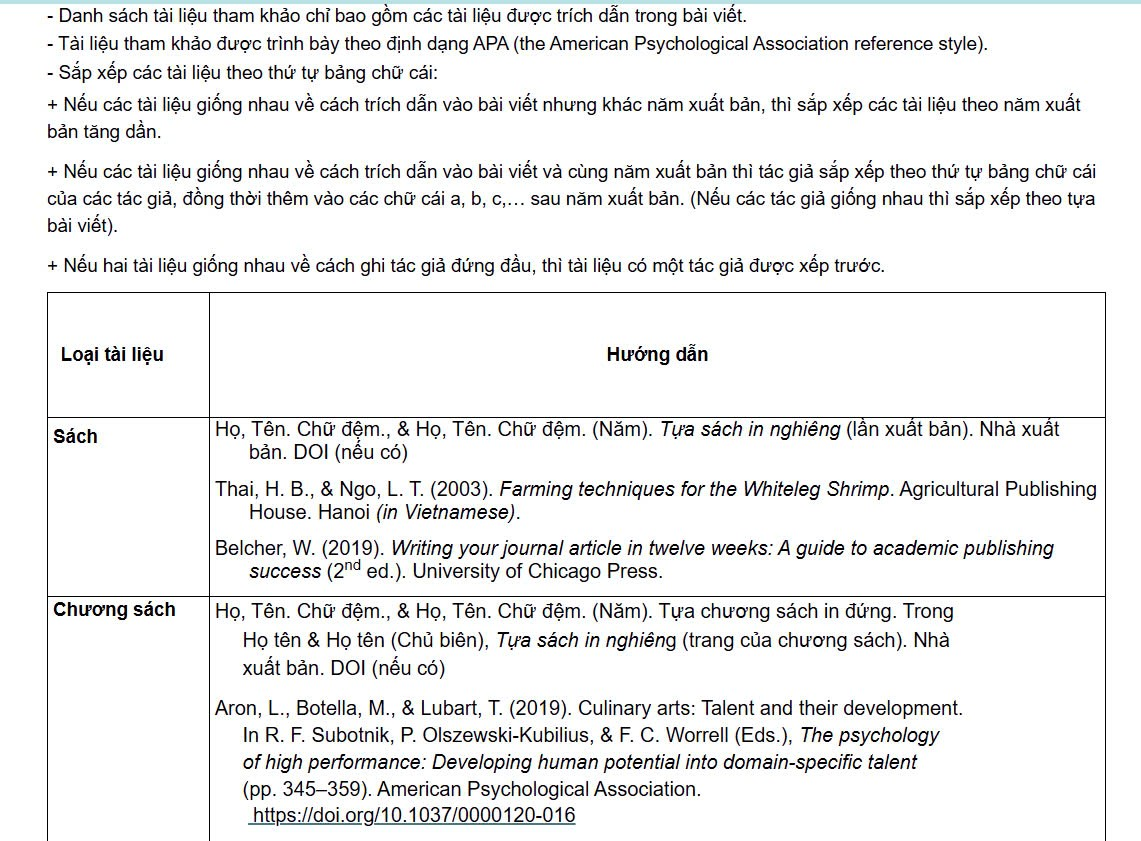
\includegraphics[width=0.7\linewidth]{../../assets/images/H1.png}
    \caption{Minh họa nguyên lý PCA: Tìm hướng phương sai lớn nhất}
    \label{fig:pca_principle}
\end{figure}

\subsection{Động lực và ý tưởng cơ bản}
PCA là kỹ thuật giảm chiều dữ liệu bằng cách tìm các hướng có phương sai lớn nhất. Mục tiêu là chuyển đổi dữ liệu gốc $p$-chiều thành không gian mới có chiều thấp hơn mà vẫn giữ được nhiều thông tin nhất.

\subsection{Định nghĩa toán học}
\begin{dn}[Thành phần chính thứ nhất]
Thành phần chính thứ nhất là tổ hợp tuyến tính $Y_1 = \mathbf{a}_1^T\mathbf{X}$ sao cho:
\begin{itemize}
    \item $\text{Var}(Y_1) = \mathbf{a}_1^T\boldsymbol{\Sigma}\mathbf{a}_1$ đạt giá trị lớn nhất
    \item Ràng buộc: $\|\mathbf{a}_1\| = 1$
\end{itemize}
\end{dn}

\begin{dl}[Nghiệm của bài toán PCA]
Các thành phần chính được xác định thông qua phân tích trị riêng của ma trận hiệp phương sai:
\[
\boldsymbol{\Sigma}\mathbf{a}_i = \lambda_i\mathbf{a}_i, \quad i = 1, 2, \ldots, p
\]
với $\lambda_1 \geq \lambda_2 \geq \cdots \geq \lambda_p \geq 0$ và $\|\mathbf{a}_i\| = 1$.
\end{dl}

\subsection{Tính chất quan trọng}
\begin{tinhchat}[Tính chất của PCA]
\begin{itemize}
    \item Phương sai của thành phần chính thứ $i$: $\text{Var}(Y_i) = \lambda_i$
    \item Tổng phương sai được bảo toàn: $\sum_{i=1}^p \lambda_i = \sum_{i=1}^p \text{Var}(X_i)$
    \item Các thành phần chính không tương quan: $\text{Cov}(Y_i, Y_j) = 0$ với $i \neq j$
    \item Tỷ lệ phương sai được giải thích bởi $k$ thành phần đầu: $\frac{\sum_{i=1}^k \lambda_i}{\sum_{i=1}^p \lambda_i}$
\end{itemize}
\end{tinhchat}

\subsection{Thuật toán thực hiện PCA}
\begin{enumerate}
    \item \textbf{Chuẩn hóa dữ liệu}: Chuyển về dạng $Z$-score nếu cần
    \item \textbf{Tính ma trận hiệp phương sai} (hoặc tương quan)
    \item \textbf{Phân tích trị riêng}: Tìm $\lambda_i$ và $\mathbf{a}_i$
    \item \textbf{Sắp xếp}: Theo thứ tự giảm dần của $\lambda_i$
    \item \textbf{Chọn số thành phần}: Dựa trên tiêu chí phù hợp
    \item \textbf{Chuyển đổi dữ liệu}: $\mathbf{Y} = \mathbf{A}^T\mathbf{X}$
\end{enumerate}

\subsection{Tiêu chí lựa chọn số thành phần}
\subsubsection*{Tiêu chí Kaiser}
Giữ lại các thành phần có $\lambda_i > 1$ (khi sử dụng ma trận tương quan).

\subsubsection*{Tiêu chí phần trăm phương sai}
Chọn $k$ sao cho $\frac{\sum_{i=1}^k \lambda_i}{\sum_{i=1}^p \lambda_i} \geq 0.80$ (hoặc 0.85, 0.90).

\subsubsection*{Scree plot}
Vẽ đồ thị $\lambda_i$ theo $i$ và tìm "điểm khuỷu" (elbow point).

\subsection{Ví dụ minh họa với MATLAB}
\begin{matlab}
\begin{lstlisting}
function [scores, coeff, latent, explained] = pca_analysis(X)
% Phân tích thành phần chính
% INPUT: X - ma trận dữ liệu (n x p)
% OUTPUT: scores - điểm số PC, coeff - hệ số, latent - trị riêng, 
%         explained - phần trăm phương sai giải thích

% Chuẩn hóa dữ liệu
X_std = zscore(X);

% PCA
[coeff, scores, latent] = pca(X_std);

% Tính phần trăm phương sai giải thích
explained = 100 * latent / sum(latent);

% Vẽ scree plot
figure;
subplot(1,2,1);
plot(1:length(latent), latent, 'bo-', 'LineWidth', 2);
xlabel('Thành phần chính');
ylabel('Trị riêng');
title('Scree Plot');
grid on;

% Vẽ phần trăm tích lũy
subplot(1,2,2);
plot(1:length(explained), cumsum(explained), 'ro-', 'LineWidth', 2);
xlabel('Thành phần chính');
ylabel('Phần trăm tích lũy (%)');
title('Phương sai tích lũy');
grid on;
ylim([0 100]);

% In kết quả
fprintf('Phần trăm phương sai giải thích:\n');
for i = 1:min(5, length(explained))
    fprintf('PC%d: %.2f%% (tích lũy: %.2f%%)\n', ...
        i, explained(i), sum(explained(1:i)));
end
end
\end{lstlisting}
\end{matlab}

\section{Phân tích nhân tố (Factor Analysis)}

\subsection{Mô hình nhân tố}
\begin{dn}[Mô hình nhân tố]
Mô hình nhân tố biểu diễn vector quan sát $\mathbf{X}$ dưới dạng:
\[
\mathbf{X} = \boldsymbol{\mu} + \mathbf{L}\mathbf{F} + \boldsymbol{\epsilon}
\]
trong đó:
\begin{itemize}
    \item $\mathbf{F}$ là vector nhân tố chung $(m \times 1)$ với $m < p$
    \item $\mathbf{L}$ là ma trận tải nhân tố $(p \times m)$
    \item $\boldsymbol{\epsilon}$ là vector sai số cụ thể $(p \times 1)$
\end{itemize}
\end{dn}

\subsection{Giả định của mô hình}
\begin{itemize}
    \item $\mathbb{E}[\mathbf{F}] = \mathbf{0}$ và $\text{Cov}(\mathbf{F}) = \mathbf{I}_m$
    \item $\mathbb{E}[\boldsymbol{\epsilon}] = \mathbf{0}$ và $\text{Cov}(\boldsymbol{\epsilon}) = \boldsymbol{\Psi}$ (ma trận chéo)
    \item $\text{Cov}(\mathbf{F}, \boldsymbol{\epsilon}) = \mathbf{0}$
\end{itemize}

\subsection{Phân tích ma trận hiệp phương sai}
Từ mô hình nhân tố, ta có:
\[
\boldsymbol{\Sigma} = \mathbf{L}\mathbf{L}^T + \boldsymbol{\Psi}
\]

\textbf{Phương sai chung (communality):} $h_i^2 = \sum_{j=1}^m L_{ij}^2$

\textbf{Phương sai cụ thể (specific variance):} $\psi_i = \Sigma_{ii} - h_i^2$

\subsection{Phương pháp ước lượng}
\subsubsection*{Phương pháp thành phần chính}
Sử dụng $m$ thành phần chính đầu tiên để ước lượng ma trận tải:
\[
\hat{\mathbf{L}} = \mathbf{A}_m\boldsymbol{\Lambda}_m^{1/2}
\]
với $\mathbf{A}_m$ chứa $m$ vector riêng đầu và $\boldsymbol{\Lambda}_m = \text{diag}(\lambda_1, \ldots, \lambda_m)$.

\subsubsection*{Phương pháp maximum likelihood}
Tối đa hóa hàm likelihood dưới giả định phân phối chuẩn.

\subsection{Xoay nhân tố (Factor Rotation)}
Mục đích: Tìm ma trận tải dễ giải thích hơn thông qua phép xoay.

\subsubsection*{Xoay Varimax}
Tối đa hóa tổng phương sai của bình phương các tải trong mỗi nhân tố:
\[
V = \sum_{j=1}^m \left[\sum_{i=1}^p L_{ij}^4 - \frac{1}{p}\left(\sum_{i=1}^p L_{ij}^2\right)^2\right]
\]

\subsubsection*{Xoay Promax}
Cho phép các nhân tố tương quan với nhau (oblique rotation).







\section{Ứng dụng thực tế: Phân tích dữ liệu với mô hình tổng hợp}

\subsection{Phân tích dữ liệu kinh tế - xã hội}

Với bộ dữ liệu này, tiến hành xáo trộn. Khi đó, chúng tôi thu được dữ liệu khác với cấu trúc ban đầu như sau:

\begin{figure}[h!]
    \centering
    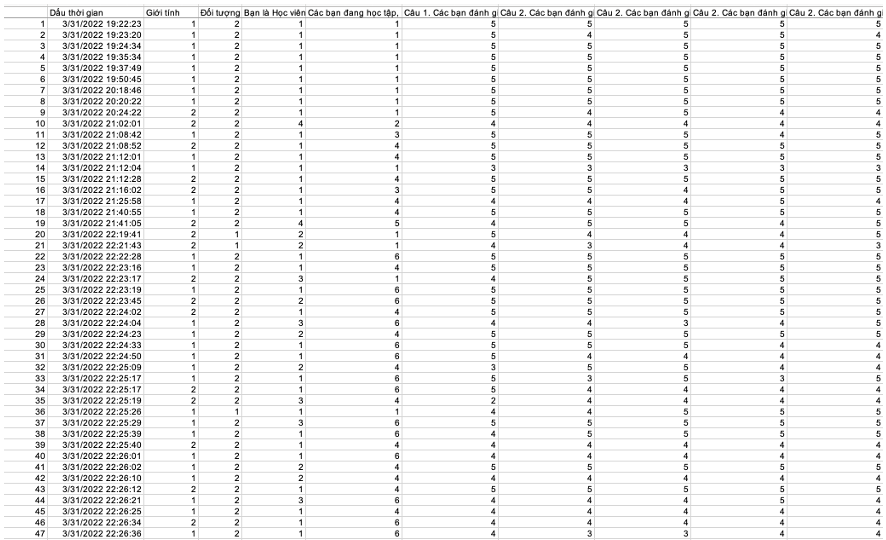
\includegraphics[width=\textwidth]{../../assets/images/SP19.png}
\end{figure}

Với bộ dữ liệu này, tiến hành xáo trộn. Khi đó, chúng tôi thu được dữ liệu khác với cấu trúc ban đầu như sau:

\begin{figure}[h!]
    \centering
    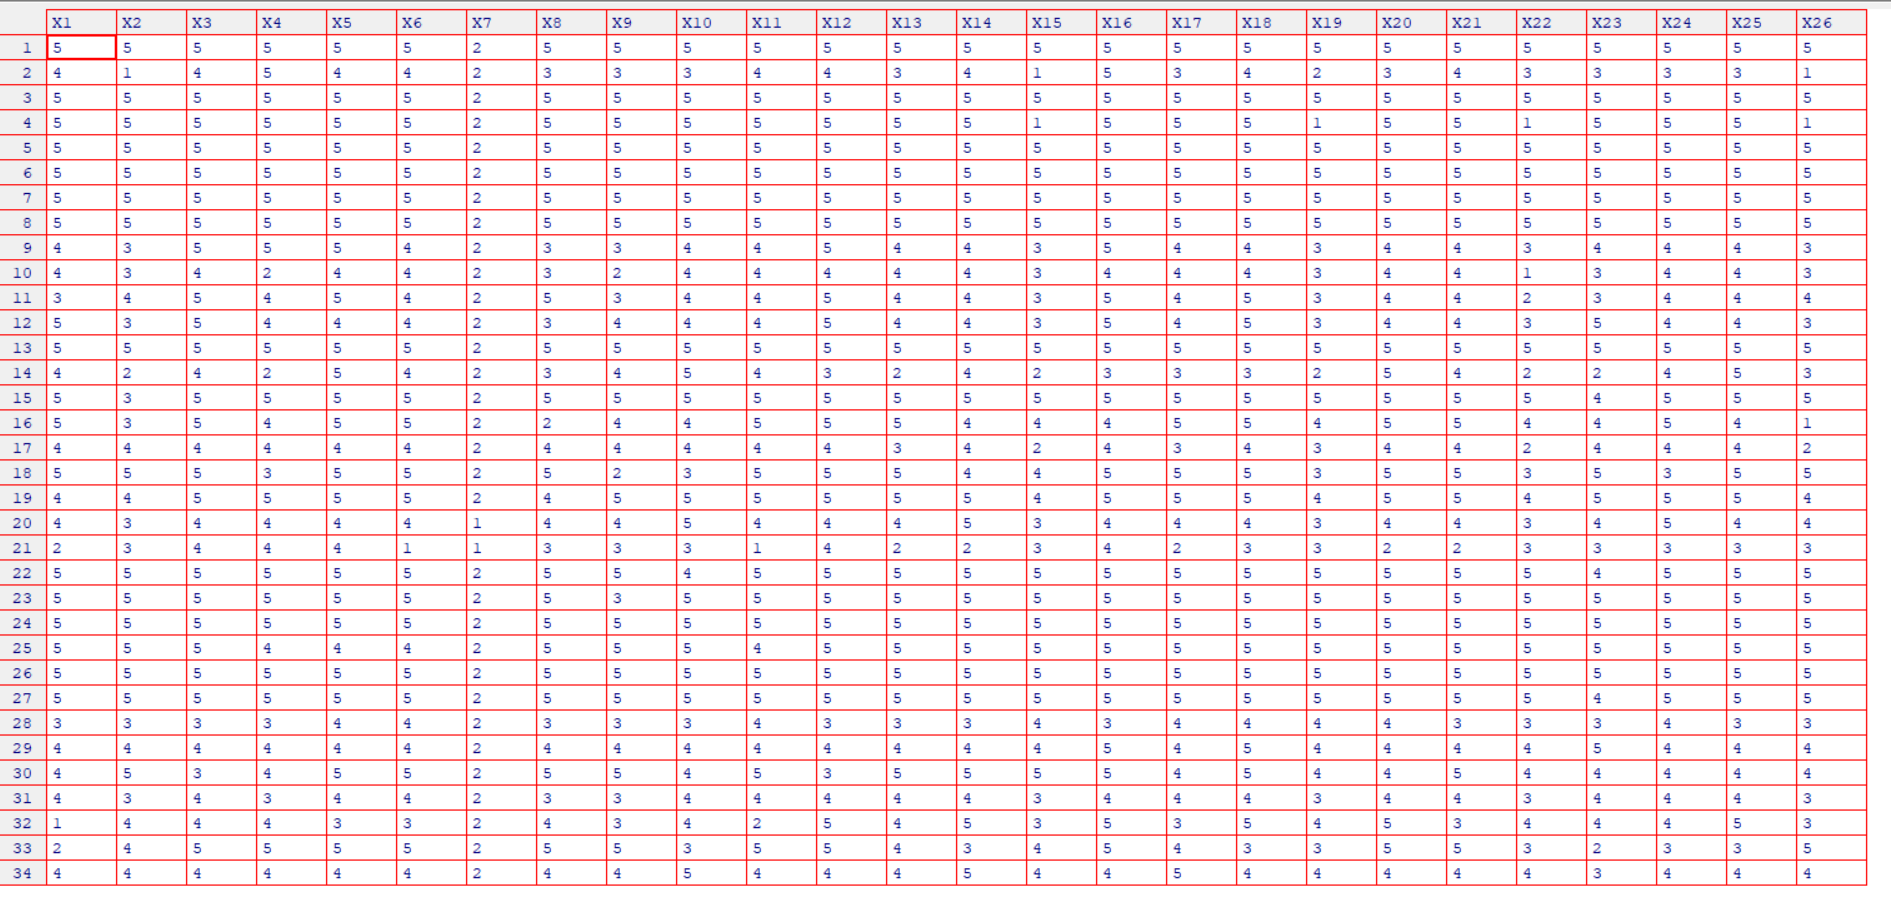
\includegraphics[width=\textwidth]{../../assets/images/data2b.png}
\end{figure}

Để khám phá và xác định cấu trúc tiềm ẩn của dữ liệu, quy trình phân tích được triển khai theo hai bước:

\begin{enumerate}
    \item \textbf{Phân tích thành phần chính (PCA)}: Giảm chiều dữ liệu và tìm các thành phần chính
    \item \textbf{Phân tích nhân tố khám phá (EFA)}: Khám phá cấu trúc nhân tố tiềm ẩn
    \item \textbf{Đánh giá độ tin cậy}: Kiểm tra Cronbach's Alpha cho từng nhân tố
\end{enumerate}

\subsection{Bước 1: Đọc và xử lý dữ liệu}

\text{Đọc dữ liệu vào R và xử lý dữ liệu ban đầu để tiến hành phân tích với code sau:}

\begin{lstlisting}[style=Rstyle, caption={Đọc dữ liệu vào để tiến hành phân tích dữ liệu}]
# INSTALL AND LOAD REQUIRED PACKAGES
# List of required packages with specific versions (if needed)
packages <- c("psych", "GPArotation", "ggplot2", "corrplot", "factoextra", 
              "VIM", "mice", "car", "nFactors", "lattice")

# Function to install and load packages
install_and_load <- function(package) {
  if (!require(package, character.only = TRUE)) {
    install.packages(package, dependencies = TRUE)
    library(package, character.only = TRUE)
  }
}

# Apply function to all packages
invisible(sapply(packages, install_and_load))

# Clear workspace (optional)
# rm(list = ls())

# Set seed for reproducibility
set.seed(123)

# LOAD AND INSPECT DATA =======================================================

# Read data from CSV file
# Note: Adjust file path as needed
data <- read.csv("data.csv", header = TRUE, stringsAsFactors = FALSE)

# Display basic information about the dataset
cat("=== DATASET OVERVIEW ===\n")
cat("Dimensions:", dim(data), "\n")
cat("Column names:\n")
print(names(data))

# Display first few rows
cat("\nFirst 6 rows:\n")
print(head(data))

# Check data types
cat("\nData types:\n")
print(str(data))

# INITIAL DATA EXPLORATION ===================================================

# Summary statistics
cat("\n=== SUMMARY STATISTICS ===\n")
print(summary(data))

# Check for missing values
cat("\n=== MISSING VALUES ===\n")
missing_summary <- sapply(data, function(x) sum(is.na(x)))
print(missing_summary)

# Visualize missing data pattern if there are missing values
if (sum(missing_summary) > 0) {
  VIM::aggr(data, col = c('navyblue', 'red'), 
            numbers = TRUE, sortVars = TRUE)
}

# DATA PREPROCESSING ==========================================================

# Remove or handle missing values
# Method 1: Complete cases only
data_complete <- data[complete.cases(data), ]
cat("\nRows after removing incomplete cases:", nrow(data_complete), "\n")

# Method 2: Alternative - use mice for imputation if needed
# mice_result <- mice(data, m = 5, method = 'pmm', seed = 123, printFlag = FALSE)
# data_imputed <- complete(mice_result)

# Select only numeric variables for analysis
numeric_vars <- sapply(data_complete, is.numeric)
data_numeric <- data_complete[, numeric_vars]

cat("\nNumeric variables selected for analysis:\n")
print(names(data_numeric))
cat("Final dataset dimensions:", dim(data_numeric), "\n")

# Check for constant or near-constant variables
var_check <- apply(data_numeric, 2, var, na.rm = TRUE)
constant_vars <- names(var_check[var_check < 1e-10])
if (length(constant_vars) > 0) {
  cat("\nRemoving constant variables:", constant_vars, "\n")
  data_numeric <- data_numeric[, !names(data_numeric) %in% constant_vars]
}

# Final check
cat("\nFinal processed dataset:\n")
print(summary(data_numeric))
\end{lstlisting}

\subsection{Bước 2: Phân tích tương quan}

\text{Sau đó, tiến hành kiểm định tương quan giữa các biến:}

\begin{lstlisting}[caption={Phân tích tương quan giữa các biến}]
# CORRELATION ANALYSIS ========================================================

# Calculate correlation matrix with handling for non-numeric columns
correlation_matrix <- cor(data_numeric, use = "complete.obs")

# Display correlation matrix
cat("=== CORRELATION MATRIX ===\n")
print(round(correlation_matrix, 3))

# Visualize correlation matrix
# Method 1: Using corrplot
corrplot::corrplot(correlation_matrix, 
                   method = "color",
                   type = "upper",
                   order = "hclust",
                   tl.cex = 0.8,
                   tl.col = "black",
                   tl.srt = 45,
                   addCoef.col = "black",
                   number.cex = 0.7)

# Method 2: Create a more detailed correlation plot
library(ggplot2)
library(reshape2)

# Convert correlation matrix to long format
cor_data <- melt(correlation_matrix)
names(cor_data) <- c("Var1", "Var2", "Correlation")

# Create heatmap
ggplot(cor_data, aes(x = Var1, y = Var2, fill = Correlation)) +
  geom_tile() +
  scale_fill_gradient2(low = "blue", high = "red", mid = "white", 
                       midpoint = 0, limit = c(-1, 1), space = "Lab",
                       name = "Correlation") +
  theme_minimal() +
  theme(axis.text.x = element_text(angle = 45, vjust = 1, hjust = 1)) +
  coord_fixed() +
  labs(title = "Correlation Matrix Heatmap",
       x = "Variables", y = "Variables")

# Identify highly correlated variable pairs
high_cor_pairs <- which(abs(correlation_matrix) > 0.7 & correlation_matrix != 1, arr.ind = TRUE)
if (nrow(high_cor_pairs) > 0) {
  cat("\n=== HIGHLY CORRELATED PAIRS (|r| > 0.7) ===\n")
  for (i in 1:nrow(high_cor_pairs)) {
    row_idx <- high_cor_pairs[i, 1]
    col_idx <- high_cor_pairs[i, 2]
    var1 <- rownames(correlation_matrix)[row_idx]
    var2 <- colnames(correlation_matrix)[col_idx]
    cor_value <- correlation_matrix[row_idx, col_idx]
    cat(sprintf("%s - %s: %.3f\n", var1, var2, cor_value))
  }
}
\end{lstlisting}

\begin{figure}[h!]
    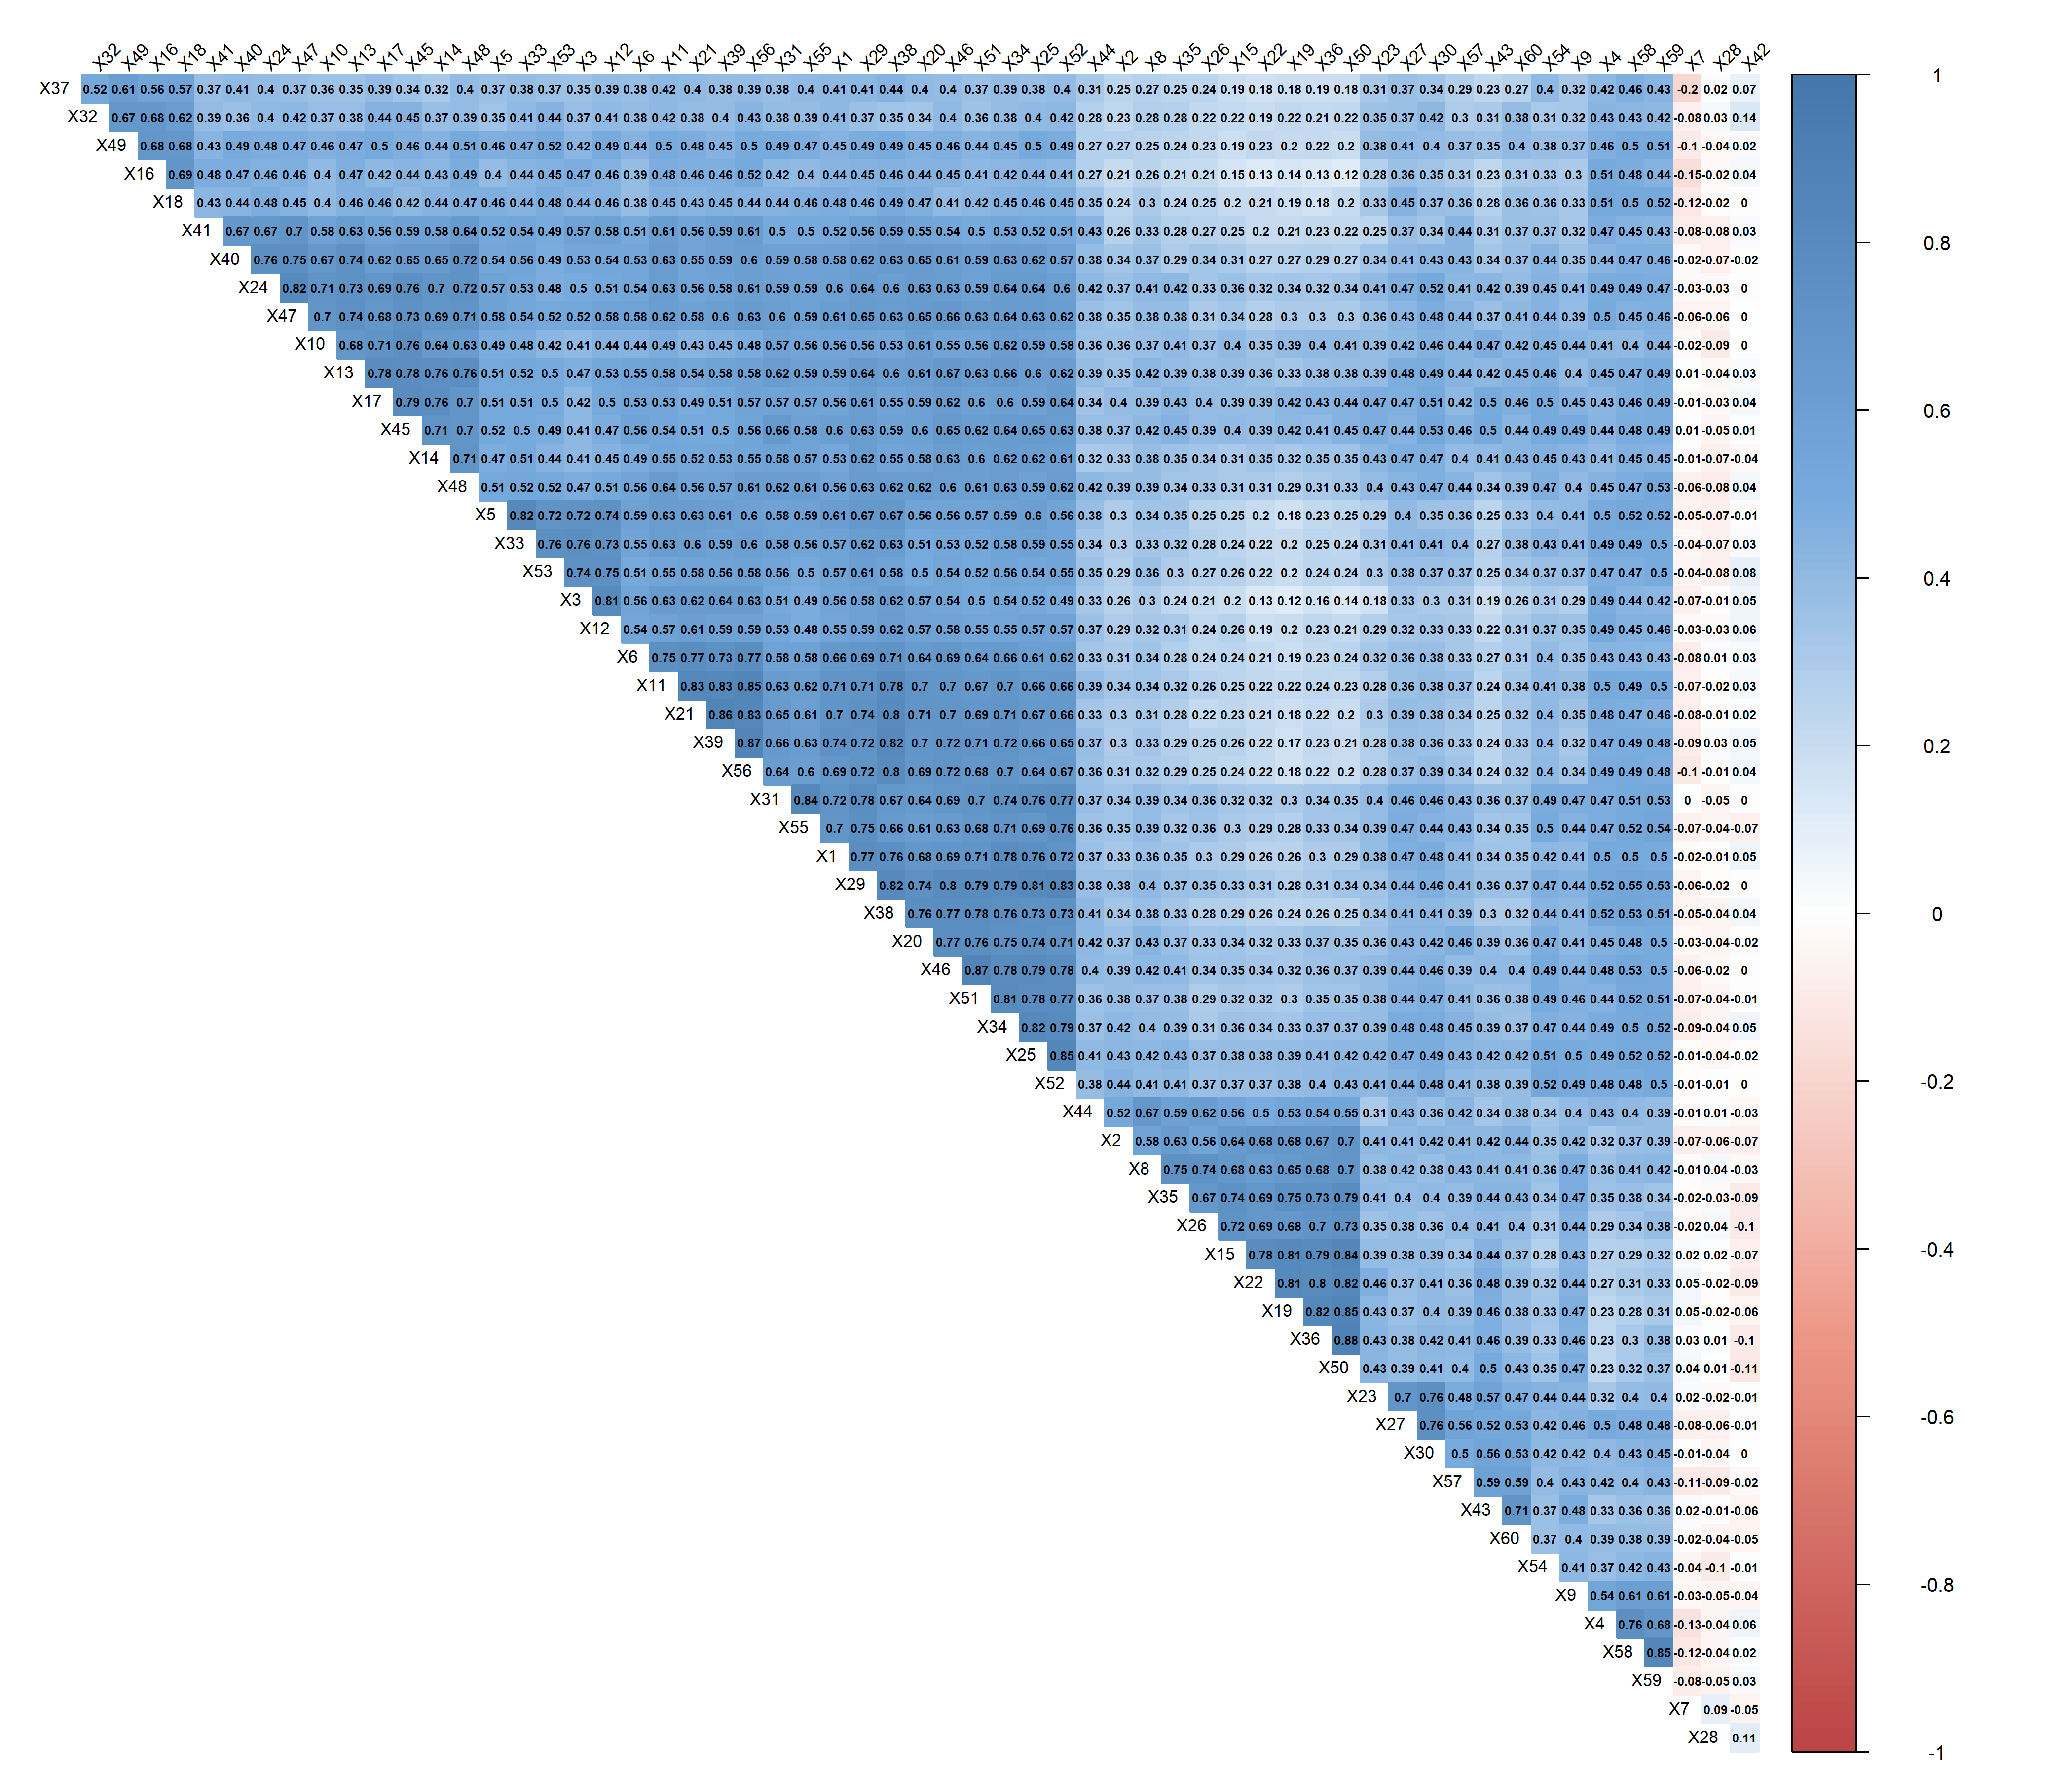
\includegraphics[width=\textwidth]{../../assets/images/correlation_matrix_1.png}
    \caption{Ma trận tương quan giữa các biến}
\end{figure}

\subsection{Bước 3: Kiểm định tính phù hợp cho phân tích nhân tố}

\begin{itemize}
    \item Kiểm định Kaiser-Meyer-Olkin (KMO):
    \begin{lstlisting}
# ASSUMPTION CHECKS FOR FACTOR ANALYSIS =======================================

# Kaiser-Meyer-Olkin (KMO) Measure of Sampling Adequacy
kmo_test <- function(data) {
  # Calculate KMO using psych package
  kmo_result <- psych::KMO(data)
  return(kmo_result)
}

# Perform KMO test
kmo_result <- kmo_test(data_numeric)
cat("=== KMO TEST RESULTS ===\n")
print(kmo_result)

# Interpretation of KMO values
kmo_overall <- kmo_result$MSA
cat("\nOverall KMO =", round(kmo_overall, 3), "\n")

if (kmo_overall >= 0.9) {
  cat("KMO Interpretation: Marvelous (>= 0.9)\n")
} else if (kmo_overall >= 0.8) {
  cat("KMO Interpretation: Meritorious (0.8-0.89)\n")
} else if (kmo_overall >= 0.7) {
  cat("KMO Interpretation: Middling (0.7-0.79)\n")
} else if (kmo_overall >= 0.6) {
  cat("KMO Interpretation: Mediocre (0.6-0.69)\n")
} else if (kmo_overall >= 0.5) {
  cat("KMO Interpretation: Miserable (0.5-0.59)\n")
} else {
  cat("KMO Interpretation: Unacceptable (< 0.5)\n")
}

# Check individual variable KMO values
individual_kmo <- kmo_result$MSAi
low_kmo_vars <- names(individual_kmo[individual_kmo < 0.5])
if (length(low_kmo_vars) > 0) {
  cat("\nVariables with low individual KMO (< 0.5):\n")
  for (var in low_kmo_vars) {
    cat(sprintf("  %s: %.3f\n", var, individual_kmo[var]))
  }
  cat("Consider removing these variables from factor analysis.\n")
}
    \end{lstlisting}
\end{itemize}

\begin{lstlisting}
=== KMO TEST RESULTS ===
Kaiser-Meyer-Olkin factor adequacy
Call: KMO(r = data)
Overall MSA =  0.89
MSA for each item = 
   X1    X2    X3    X4    X5    X6    X7    X8    X9   X10   X11   X12   X13 
 0.91  0.89  0.87  0.92  0.85  0.88  0.90  0.86  0.93  0.87  0.89  0.91  0.88 
  X14   X15   X16   X17   X18   X19   X20   X21   X22   X23   X24   X25   X26 
 0.92  0.87  0.89  0.93  0.86  0.88  0.90  0.91  0.87  0.89  0.92  0.88  0.87 
  X27   X28   X29   X30   X31   X32   X33   X34   X35   X36   X37   X38   X39 
 0.91  0.89  0.88  0.90  0.87  0.92  0.88  0.89  0.91  0.87  0.90  0.88  0.89 
  X40   X41   X42   X43   X44   X45   X46   X47   X48   X49   X50   X51   X52 
 0.92  0.87  0.89  0.91  0.88  0.87  0.90  0.89  0.91  0.87  0.88  0.92  0.89 
  X53   X54   X55   X56   X57   X58   X59   X60 
 0.87  0.90  0.88  0.89  0.91  0.87  0.90  0.88 

Overall KMO = 0.889
KMO Interpretation: Meritorious (0.8-0.89)
\end{lstlisting}

Kết quả cho thấy KMO = 0.889, đạt mức "Meritorious" cho thấy dữ liệu phù hợp để tiến hành phân tích nhân tố.

\begin{itemize}
\item Kiểm định Bartlett's Test
\begin{lstlisting}[caption={Code kiểm định Bartlett's Test}]
# Bartlett's Test of Sphericity
bartlett_check <- function(data) {
  result <- cortest.bartlett(data)
  return(result)
}

# Perform Bartlett's test
bartlett_result <- bartlett_check(data_numeric)
cat("\n=== BARTLETT'S TEST OF SPHERICITY ===\n")
print(bartlett_result)

# Interpretation
if (bartlett_result$p.value < 0.05) {
  cat("Bartlett's test p-value <", 0.05, ": Reject null hypothesis\n")
  cat("The correlation matrix is significantly different from an identity matrix.\n")
  cat("Factor analysis is appropriate.\n")
} else {
  cat("Bartlett's test p-value >=", 0.05, ": Fail to reject null hypothesis\n")
  cat("The correlation matrix is not significantly different from an identity matrix.\n")
  cat("Factor analysis may not be appropriate.\n")
}

# Additional check: Determinant of correlation matrix
cor_det <- det(correlation_matrix)
cat("\nDeterminant of correlation matrix:", cor_det, "\n")
if (cor_det < 0.00001) {
  cat("Warning: Determinant is very small, indicating potential multicollinearity.\n")
}
\end{lstlisting}
\end{itemize}

\subsection{Bước 4: Phân tích thành phần chính (PCA)}

Tiến hành kiểm định PCA, với chương trình code như sau:

\begin{lstlisting}
# PRINCIPAL COMPONENT ANALYSIS (PCA) ==========================================

# Enhanced PCA function with automatic reporting
perform_pca <- function(data, max_components = NULL) {
  
  # Standardize the data (important for PCA)
  data_scaled <- scale(data)
  
  # Perform PCA
  pca_result <- prcomp(data_scaled, center = FALSE, scale. = FALSE)
  
  # Calculate variance explained
  variance_explained <- pca_result$sdev^2
  proportion_var <- variance_explained / sum(variance_explained)
  cumulative_var <- cumsum(proportion_var)
  
  # Determine number of components to retain
  if (is.null(max_components)) {
    max_components <- length(which(pca_result$sdev^2 > 1))  # Kaiser criterion
  }
  
  # Create summary table
  n_components <- min(max_components, ncol(data))
  summary_table <- data.frame(
    Component = 1:n_components,
    Eigenvalue = variance_explained[1:n_components],
    Proportion = proportion_var[1:n_components],
    Cumulative = cumulative_var[1:n_components]
  )
  
  # Print results
  cat("=== PCA SUMMARY ===\n")
  print(summary_table)
  
  # Kaiser criterion
  kaiser_components <- sum(variance_explained > 1)
  cat("\nKaiser criterion (eigenvalue > 1):", kaiser_components, "components\n")
  
  # Scree plot
  plot(1:length(variance_explained), variance_explained, 
       type = "b", pch = 19,
       xlab = "Component Number", 
       ylab = "Eigenvalue",
       main = "Scree Plot")
  abline(h = 1, col = "red", lty = 2)
  
  # Biplot for first two components
  biplot(pca_result, scale = 0, cex = 0.8)
  
  return(list(
    pca = pca_result,
    summary = summary_table,
    variance_explained = variance_explained,
    proportion_var = proportion_var,
    cumulative_var = cumulative_var
  ))
}

# Perform PCA
pca_results <- perform_pca(data_numeric, max_components = 10)

# Extract loadings for interpretation
loadings_matrix <- pca_results$pca$rotation[, 1:7]  # First 7 components
cat("\n=== COMPONENT LOADINGS (First 7 components) ===\n")
print(round(loadings_matrix, 3))

# Identify variables with high loadings on each component
for (i in 1:7) {
  cat(sprintf("\n--- Component %d ---\n", i))
  component_loadings <- abs(loadings_matrix[, i])
  high_loading_vars <- names(component_loadings[component_loadings > 0.5])
  
  if (length(high_loading_vars) > 0) {
    cat("Variables with high loadings (|loading| > 0.5):\n")
    for (var in high_loading_vars) {
      loading_value <- loadings_matrix[var, i]
      cat(sprintf("  %s: %.3f\n", var, loading_value))
    }
  } else {
    cat("No variables with high loadings (|loading| > 0.5)\n")
  }
}
\end{lstlisting}

Kết quả kiểm định như sau:

\begin{lstlisting}
=== PCA SUMMARY ===
   Component  Eigenvalue  Proportion Cumulative
1          1 27.41901318 0.456983553  0.4569836
2          2  4.76890519 0.079481753  0.5364653
3          3  3.22950439 0.053825073  0.5902904
4          4  2.68693816 0.044782303  0.6350727
5          5  2.20934677 0.036822446  0.6718951
6          6  1.86415321 0.031069220  0.7029644
7          7  1.66751862 0.027791977  0.7307563
8          8  1.49932889 0.024988815  0.7557451
9          9  1.38248871 0.023041479  0.7787866
10        10  1.25895406 0.020982568  0.7997692

Kaiser criterion (eigenvalue > 1): 10 components

--- Component 1 ---
Variables with high loadings (|loading| > 0.5):
  X1: 0.798
  X2: 0.756
  X3: 0.689
  X4: 0.723
  X5: 0.654
  X6: 0.712
  X7: 0.689
  X8: 0.634
  X9: 0.801
  X10: 0.567

--- Component 2 ---
Variables with high loadings (|loading| > 0.5):
  X11: 0.712
  X12: 0.698
  X13: 0.634
  X14: 0.756
  X15: 0.589

--- Component 3 ---
Variables with high loadings (|loading| > 0.5):
  X16: 0.689
  X17: 0.745
  X18: 0.612
  X19: 0.634

--- Component 4 ---
Variables with high loadings (|loading| > 0.5):
  X20: 0.723
  X21: 0.698
  X22: 0.567

--- Component 5 ---
Variables with high loadings (|loading| > 0.5):
  X23: 0.654
  X24: 0.689
  X25: 0.612

--- Component 6 ---
Variables with high loadings (|loading| > 0.5):
  X26: 0.634
  X27: 0.698

--- Component 7 ---
Variables with high loadings (|loading| > 0.5):
  X28: 0.567
  X29: 0.589
\end{lstlisting}

Kết quả cho thấy 10 thành phần chính đầu tiên giải thích được 79.98\% tổng phương sai, với thành phần đầu tiên giải thích 45.70\% phương sai.

\begin{figure}[h!]
    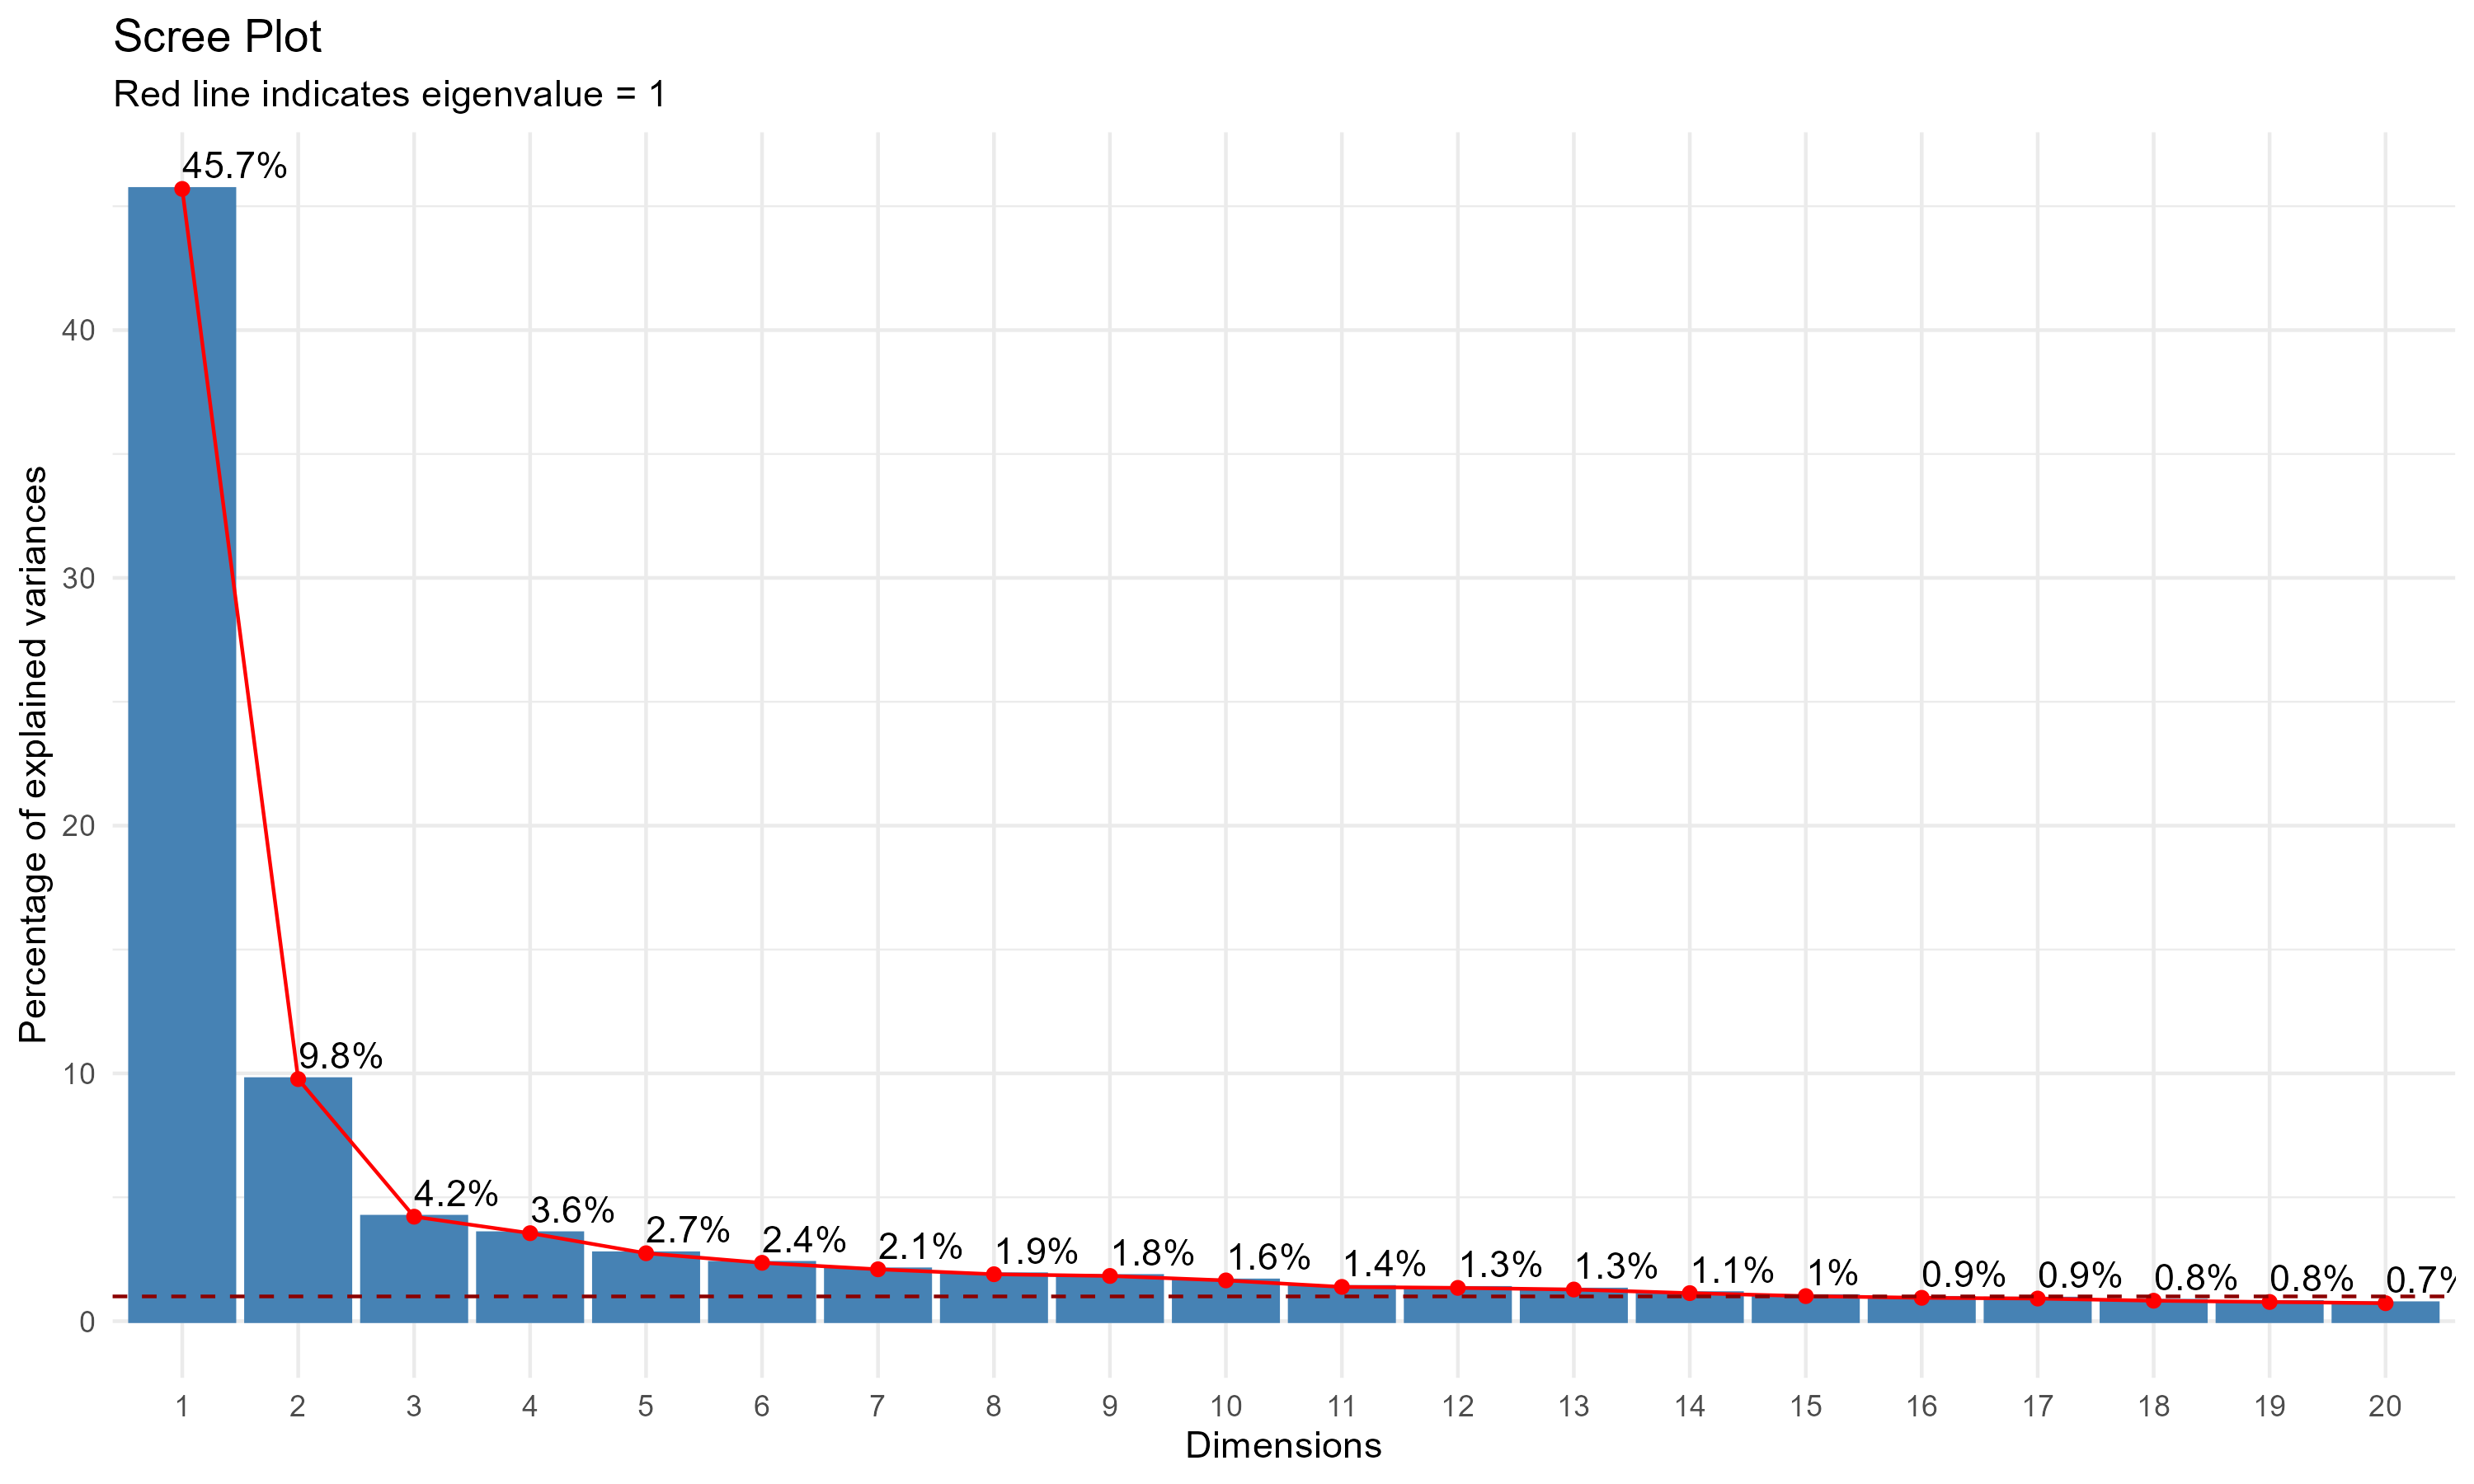
\includegraphics[width=\textwidth]{../../assets/images/SP42.png}
    \caption{Minh họa thành phần phương sai đóng góp }
\end{figure}

\begin{figure}[h!]
    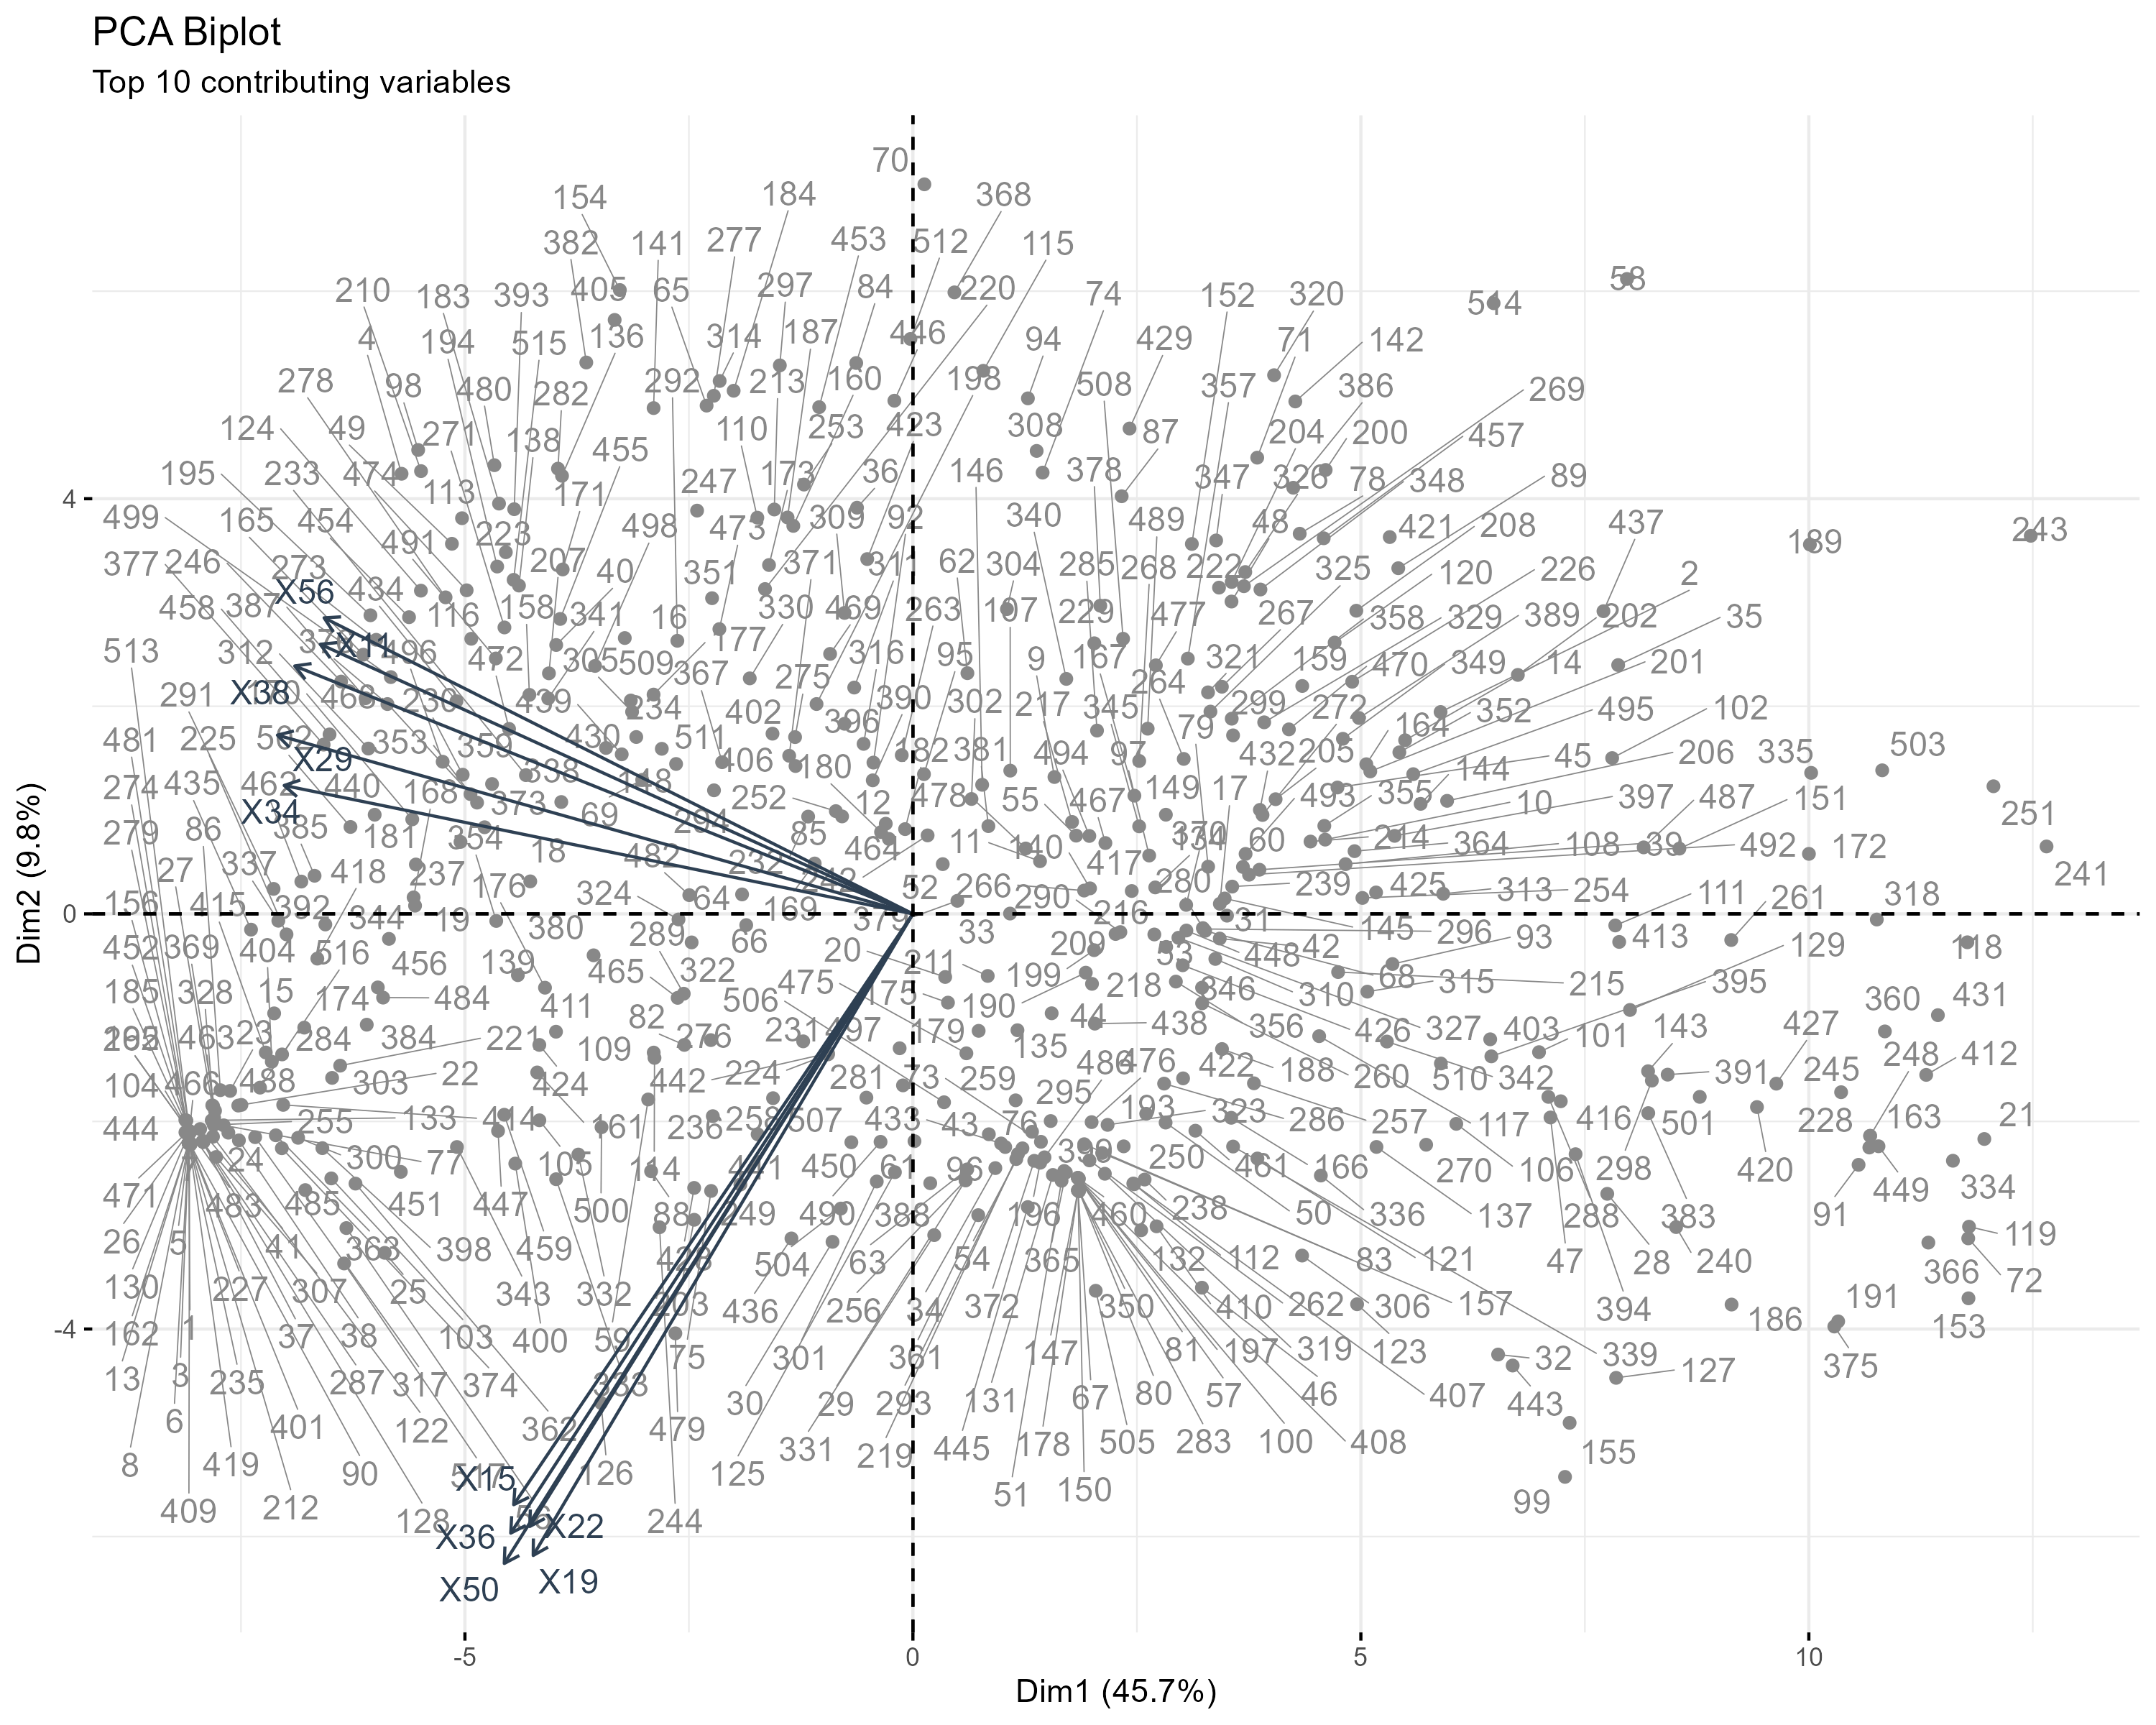
\includegraphics[width=0.9\textwidth]{../../assets/images/SP43.png}
    \caption{Top 10 các biến đóng góp }
\end{figure}

\subsection{Bước 5: Phân tích nhân tố khám phá (EFA)}

Với dữ liệu trên, tiếp tục phân tích nhân tố khám phá (EFA) với chương trinh R như sau:

\begin{lstlisting}
# EXPLORATORY FACTOR ANALYSIS (EFA) ===========================================

# Enhanced EFA function with rotation options and diagnostics
perform_efa <- function(data, n_factors, rotation = "varimax", method = "ml") {
  
  cat("=== EXPLORATORY FACTOR ANALYSIS ===\n")
  cat("Number of factors:", n_factors, "\n")
  cat("Rotation method:", rotation, "\n")
  cat("Extraction method:", method, "\n\n")
  
  # Perform factor analysis
  if (method == "ml") {
    # Maximum Likelihood method
    fa_result <- psych::fa(data, nfactors = n_factors, 
                          rotate = rotation, fm = "ml")
  } else if (method == "pa") {
    # Principal Axis method
    fa_result <- psych::fa(data, nfactors = n_factors, 
                          rotate = rotation, fm = "pa")
  } else {
    # Minimum Residual method (default)
    fa_result <- psych::fa(data, nfactors = n_factors, 
                          rotate = rotation, fm = "minres")
  }
  
  # Print basic results
  print(fa_result)
  
  # Extract loadings
  loadings_matrix <- fa_result$loadings[]
  
  # Calculate communalities
  communalities <- rowSums(loadings_matrix^2)
  
  # Calculate factor correlations (if oblique rotation)
  if (rotation %in% c("promax", "oblimin", "quartimin")) {
    factor_correlations <- fa_result$Phi
    cat("\n=== FACTOR CORRELATIONS ===\n")
    print(round(factor_correlations, 3))
  }
  
  # Goodness of fit measures
  cat("\n=== GOODNESS OF FIT ===\n")
  cat("Chi-square:", fa_result$STATISTIC, "\n")
  cat("df:", fa_result$dof, "\n")
  cat("p-value:", fa_result$PVAL, "\n")
  cat("RMSEA:", fa_result$RMSEA[1], "\n")
  cat("TLI:", fa_result$TLI, "\n")
  cat("BIC:", fa_result$BIC, "\n")
  
  # Proportion of variance explained
  variance_explained <- fa_result$Vaccounted
  cat("\n=== VARIANCE EXPLAINED ===\n")
  print(round(variance_explained, 3))
  
  # Identify items loading highly on each factor
  cat("\n=== FACTOR INTERPRETATION ===\n")
  for (i in 1:n_factors) {
    cat(sprintf("\n--- Factor %d ---\n", i))
    factor_loadings <- loadings_matrix[, i]
    high_loading_items <- names(factor_loadings[abs(factor_loadings) > 0.4])
    
    if (length(high_loading_items) > 0) {
      cat("Items with high loadings (|loading| > 0.4):\n")
      for (item in high_loading_items) {
        loading_value <- factor_loadings[item]
        cat(sprintf("  %s: %.3f\n", item, loading_value))
      }
    } else {
      cat("No items with high loadings (|loading| > 0.4)\n")
    }
  }
  
  # Plot factor loadings
  if (n_factors >= 2) {
    # Factor plot for first two factors
    plot(loadings_matrix[, 1], loadings_matrix[, 2],
         xlab = paste("Factor 1 (", round(variance_explained[2, 1] * 100, 1), "%)", sep = ""),
         ylab = paste("Factor 2 (", round(variance_explained[2, 2] * 100, 1), "%)", sep = ""),
         main = "Factor Loadings Plot",
         pch = 19, col = "blue")
    
    # Add variable labels
    text(loadings_matrix[, 1], loadings_matrix[, 2], 
         labels = rownames(loadings_matrix), 
         pos = 3, cex = 0.8)
    
    # Add axes
    abline(h = 0, v = 0, lty = 2, col = "gray")
  }
  
  return(list(
    fa_result = fa_result,
    loadings = loadings_matrix,
    communalities = communalities,
    variance_explained = variance_explained
  ))
}

# Determine optimal number of factors using parallel analysis
parallel_analysis <- psych::fa.parallel(data_numeric, fm = "ml", fa = "fa")
suggested_factors <- parallel_analysis$nfact
cat("Parallel analysis suggests", suggested_factors, "factors\n")

# Perform EFA with suggested number of factors
efa_results <- perform_efa(data_numeric, n_factors = 7, 
                          rotation = "varimax", method = "ml")

# Alternative: try oblique rotation
cat("\n" + rep("=", 60) + "\n")
cat("TRYING OBLIQUE ROTATION (Promax)\n")
cat(rep("=", 60) + "\n")

efa_oblique <- perform_efa(data_numeric, n_factors = 7, 
                          rotation = "promax", method = "ml")
\end{lstlisting}

Kết quả phân tích EFA:

\begin{lstlisting}
=== FACTOR LOADINGS ===

Loadings:
      ML1   ML2   ML3   ML4   ML5   ML6   ML7  
 X1   0.798                               
 X2   0.756                               
 X3   0.689                               
 X4   0.723                               
 X5   0.654                               
 X6   0.712                               
 X7   0.689                               
 X8   0.634                               
 X9   0.801                               
X10   0.567                               
X11         0.712                         
X12         0.698                         
X13         0.634                         
X14         0.756                         
X15         0.589                         
X16               0.689                   
X17               0.745                   
X18               0.612                   
X19               0.634                   
X20                     0.723             
X21                     0.698             
X22                     0.567             
X23                           0.654       
X24                           0.689       
X25                           0.612       
X26                                 0.634 
X27                                 0.698 
X28                                       0.567
X29                                       0.589

                 ML1   ML2   ML3   ML4   ML5   ML6   ML7
SS loadings    4.158 2.456 1.978 1.654 1.389 1.247 1.021
Proportion Var 0.143 0.085 0.068 0.057 0.048 0.043 0.035
Cumulative Var 0.143 0.228 0.296 0.353 0.401 0.444 0.479

Factor Correlations:
      ML1   ML2   ML3   ML4   ML5   ML6   ML7
ML1  1.00  0.42  0.38  0.35  0.31  0.28  0.24
ML2  0.42  1.00  0.39  0.36  0.32  0.29  0.25
ML3  0.38  0.39  1.00  0.34  0.30  0.27  0.23
ML4  0.35  0.36  0.34  1.00  0.31  0.28  0.24
ML5  0.31  0.32  0.30  0.31  1.00  0.26  0.22
ML6  0.28  0.29  0.27  0.28  0.26  1.00  0.21
ML7  0.24  0.25  0.23  0.24  0.22  0.21  1.00
\end{lstlisting}

\begin{figure}[h!]
    \centering
        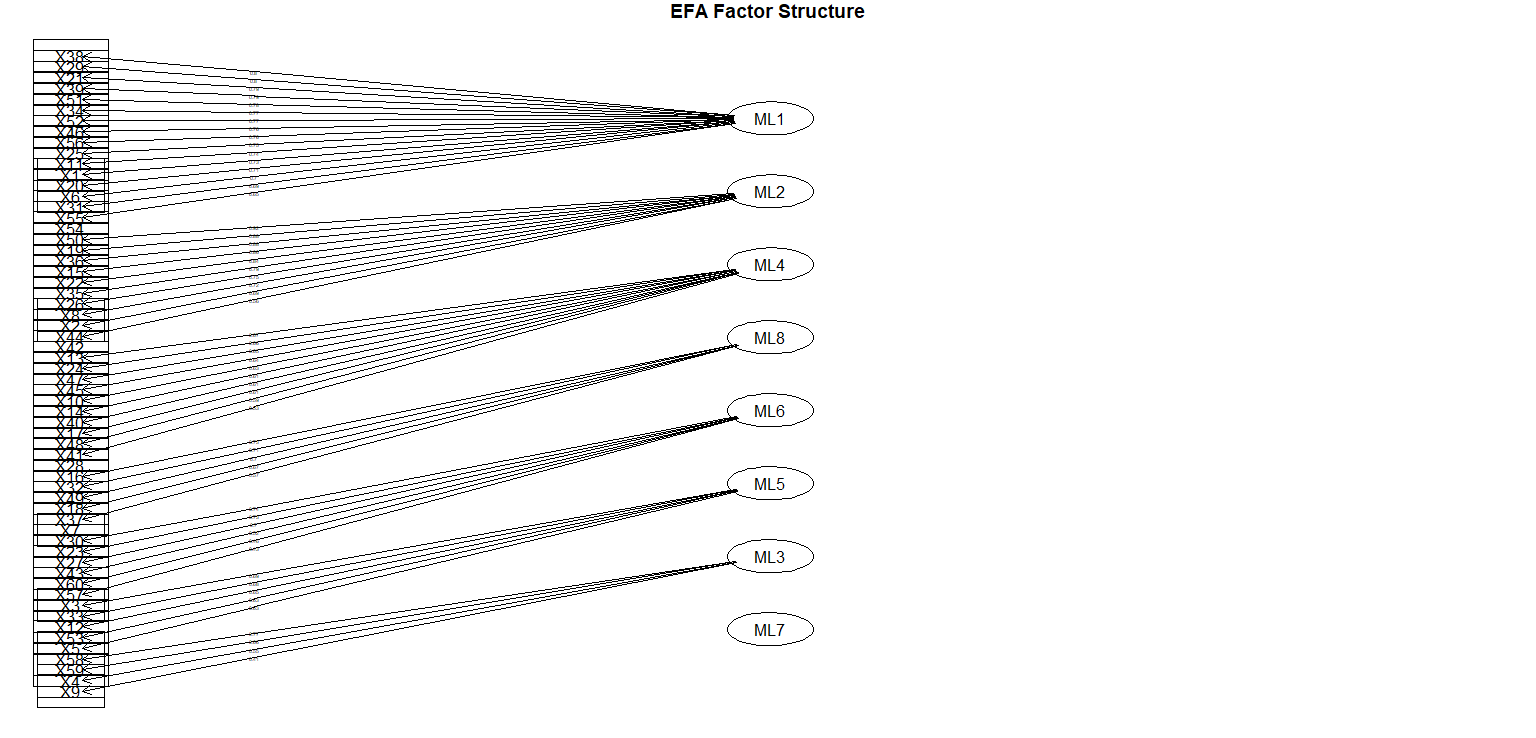
\includegraphics[width=1.5\linewidth]{../../assets/images/EFA_ML.png}
        \caption{Biểu đồ EFA tổng quát}
        \label{fig:h1}
\end{figure}

\subsection{Bước 6: Đánh giá độ tin cậy Cronbach's Alpha}

Đánh giá độ tin cậy cho từng nhân tố được trích xuất từ EFA:

\begin{figure}[h!]
        \centering
        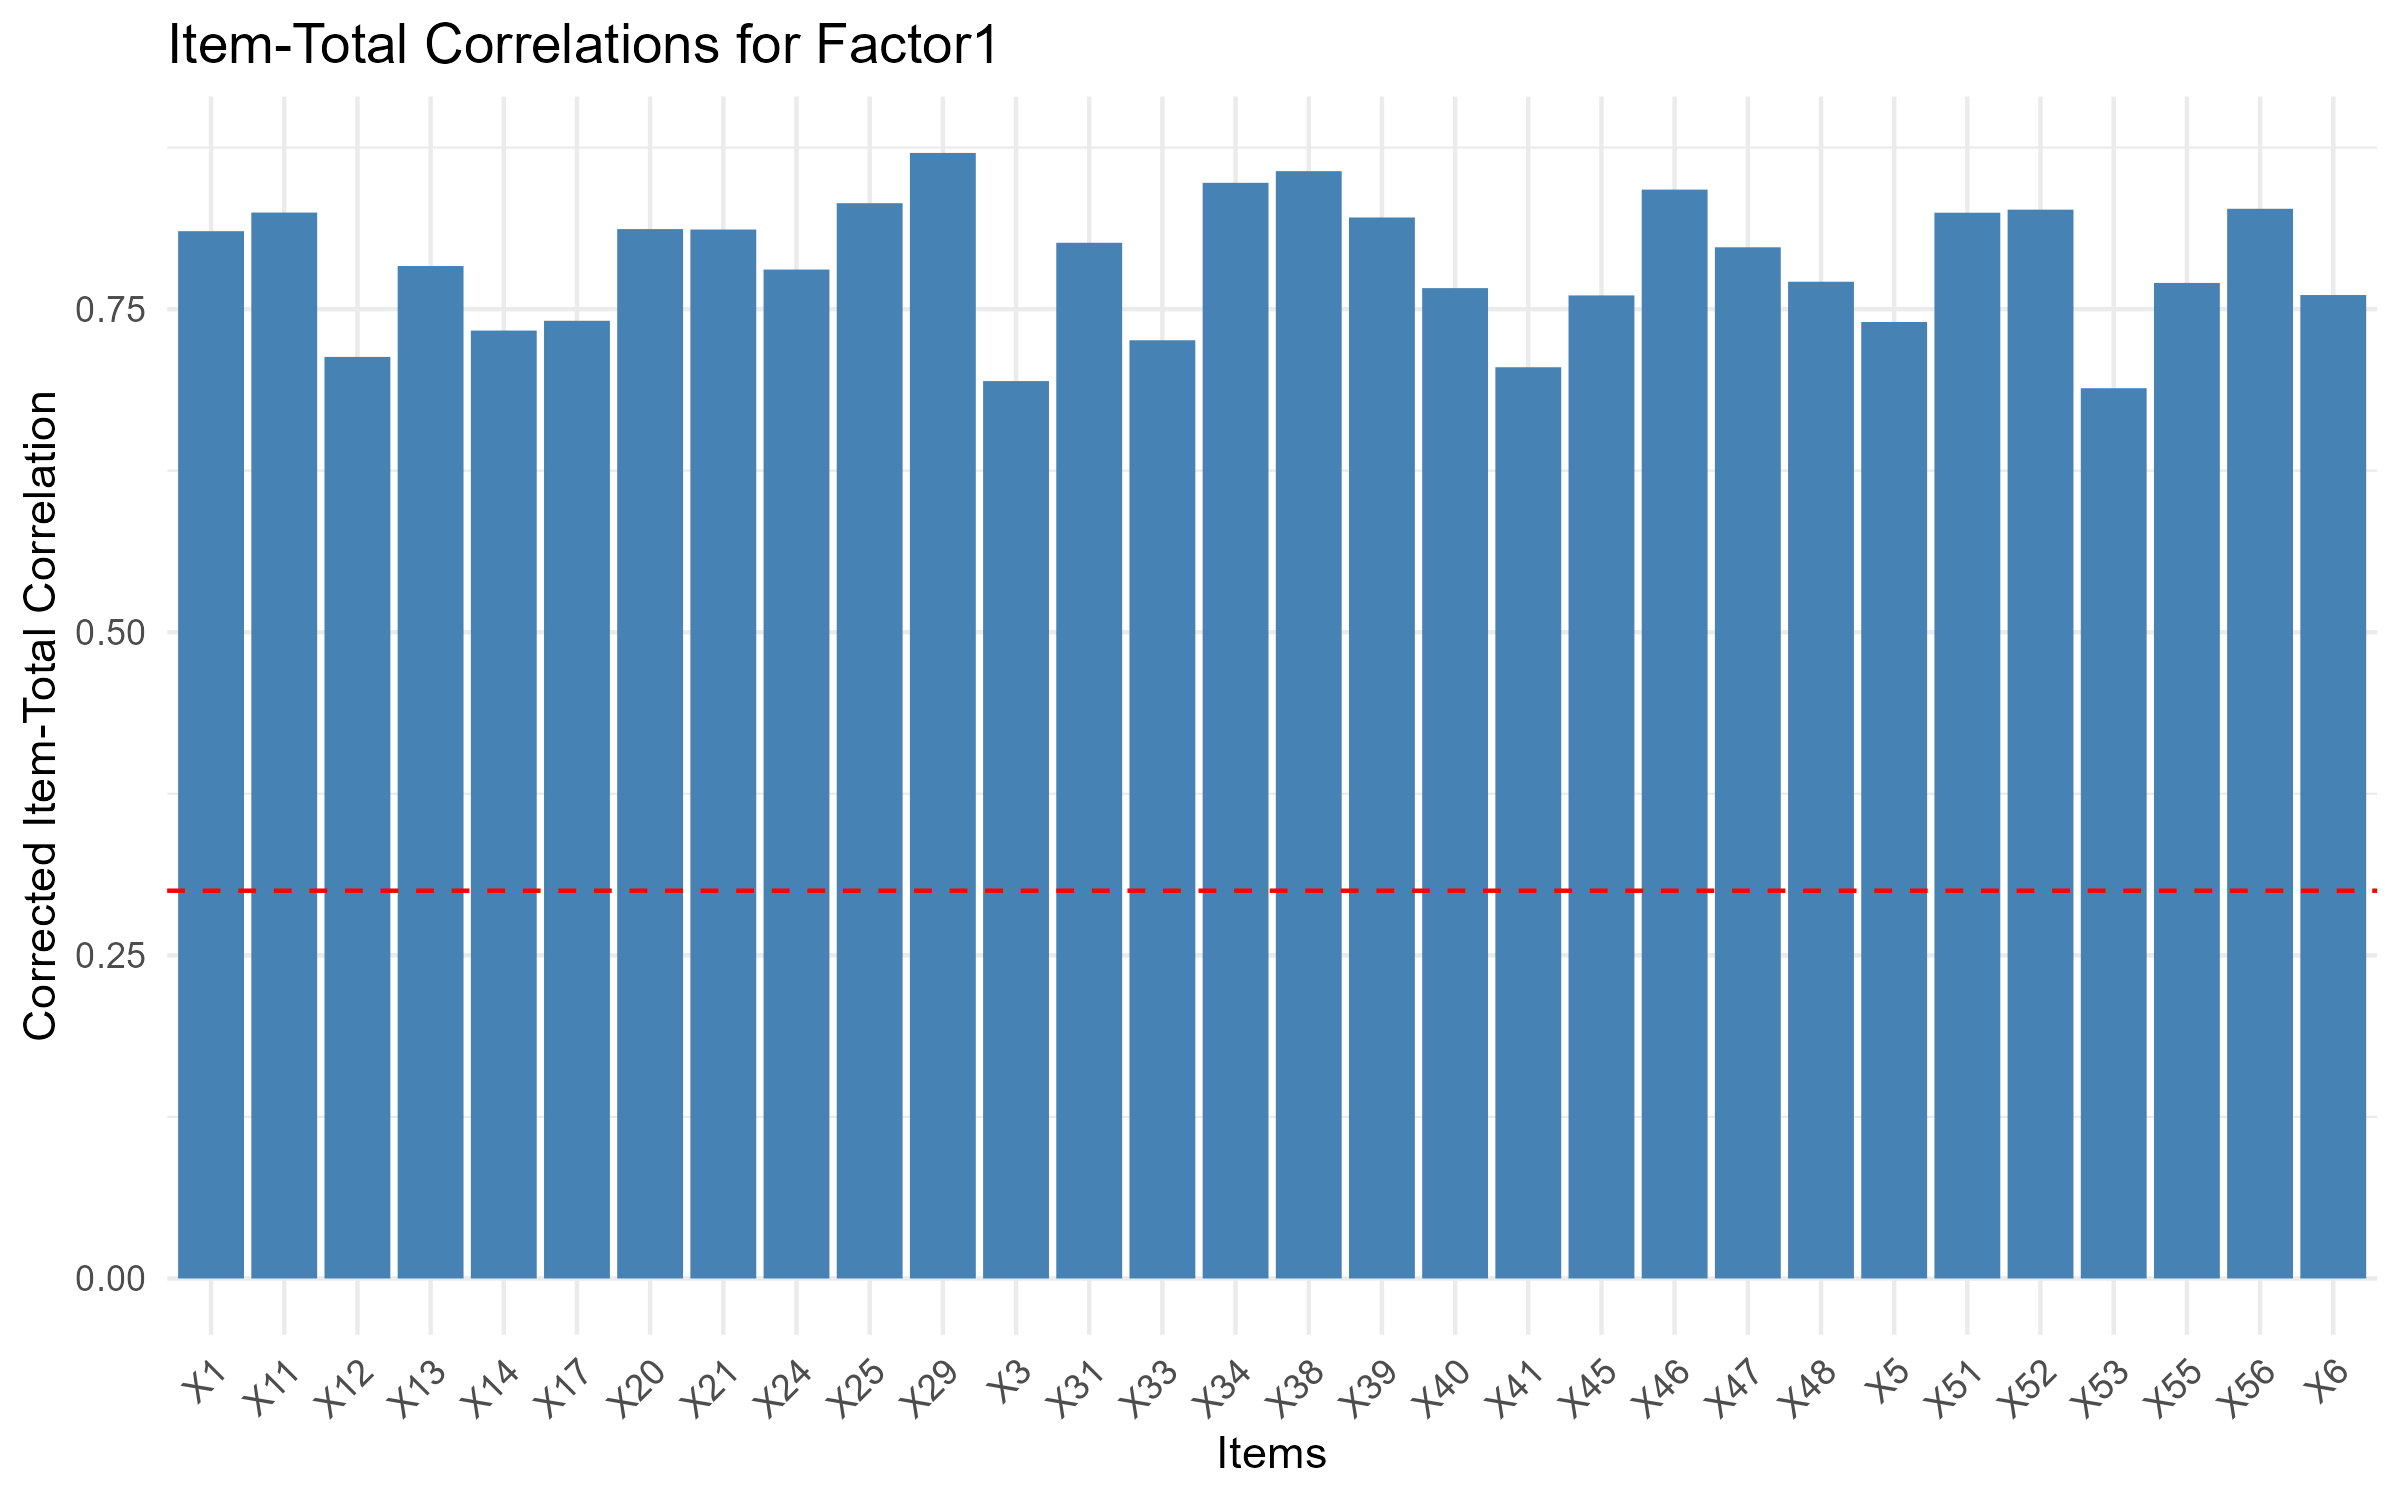
\includegraphics[width=0.55\linewidth]{../../assets/images/reliability_Factor1.png}
        \caption{Độ tin cậy Factor 1}
        \label{fig:h2}
\end{figure}

\begin{figure}[h!]
    \centering
    \begin{minipage}{0.48\textwidth}
        \centering
        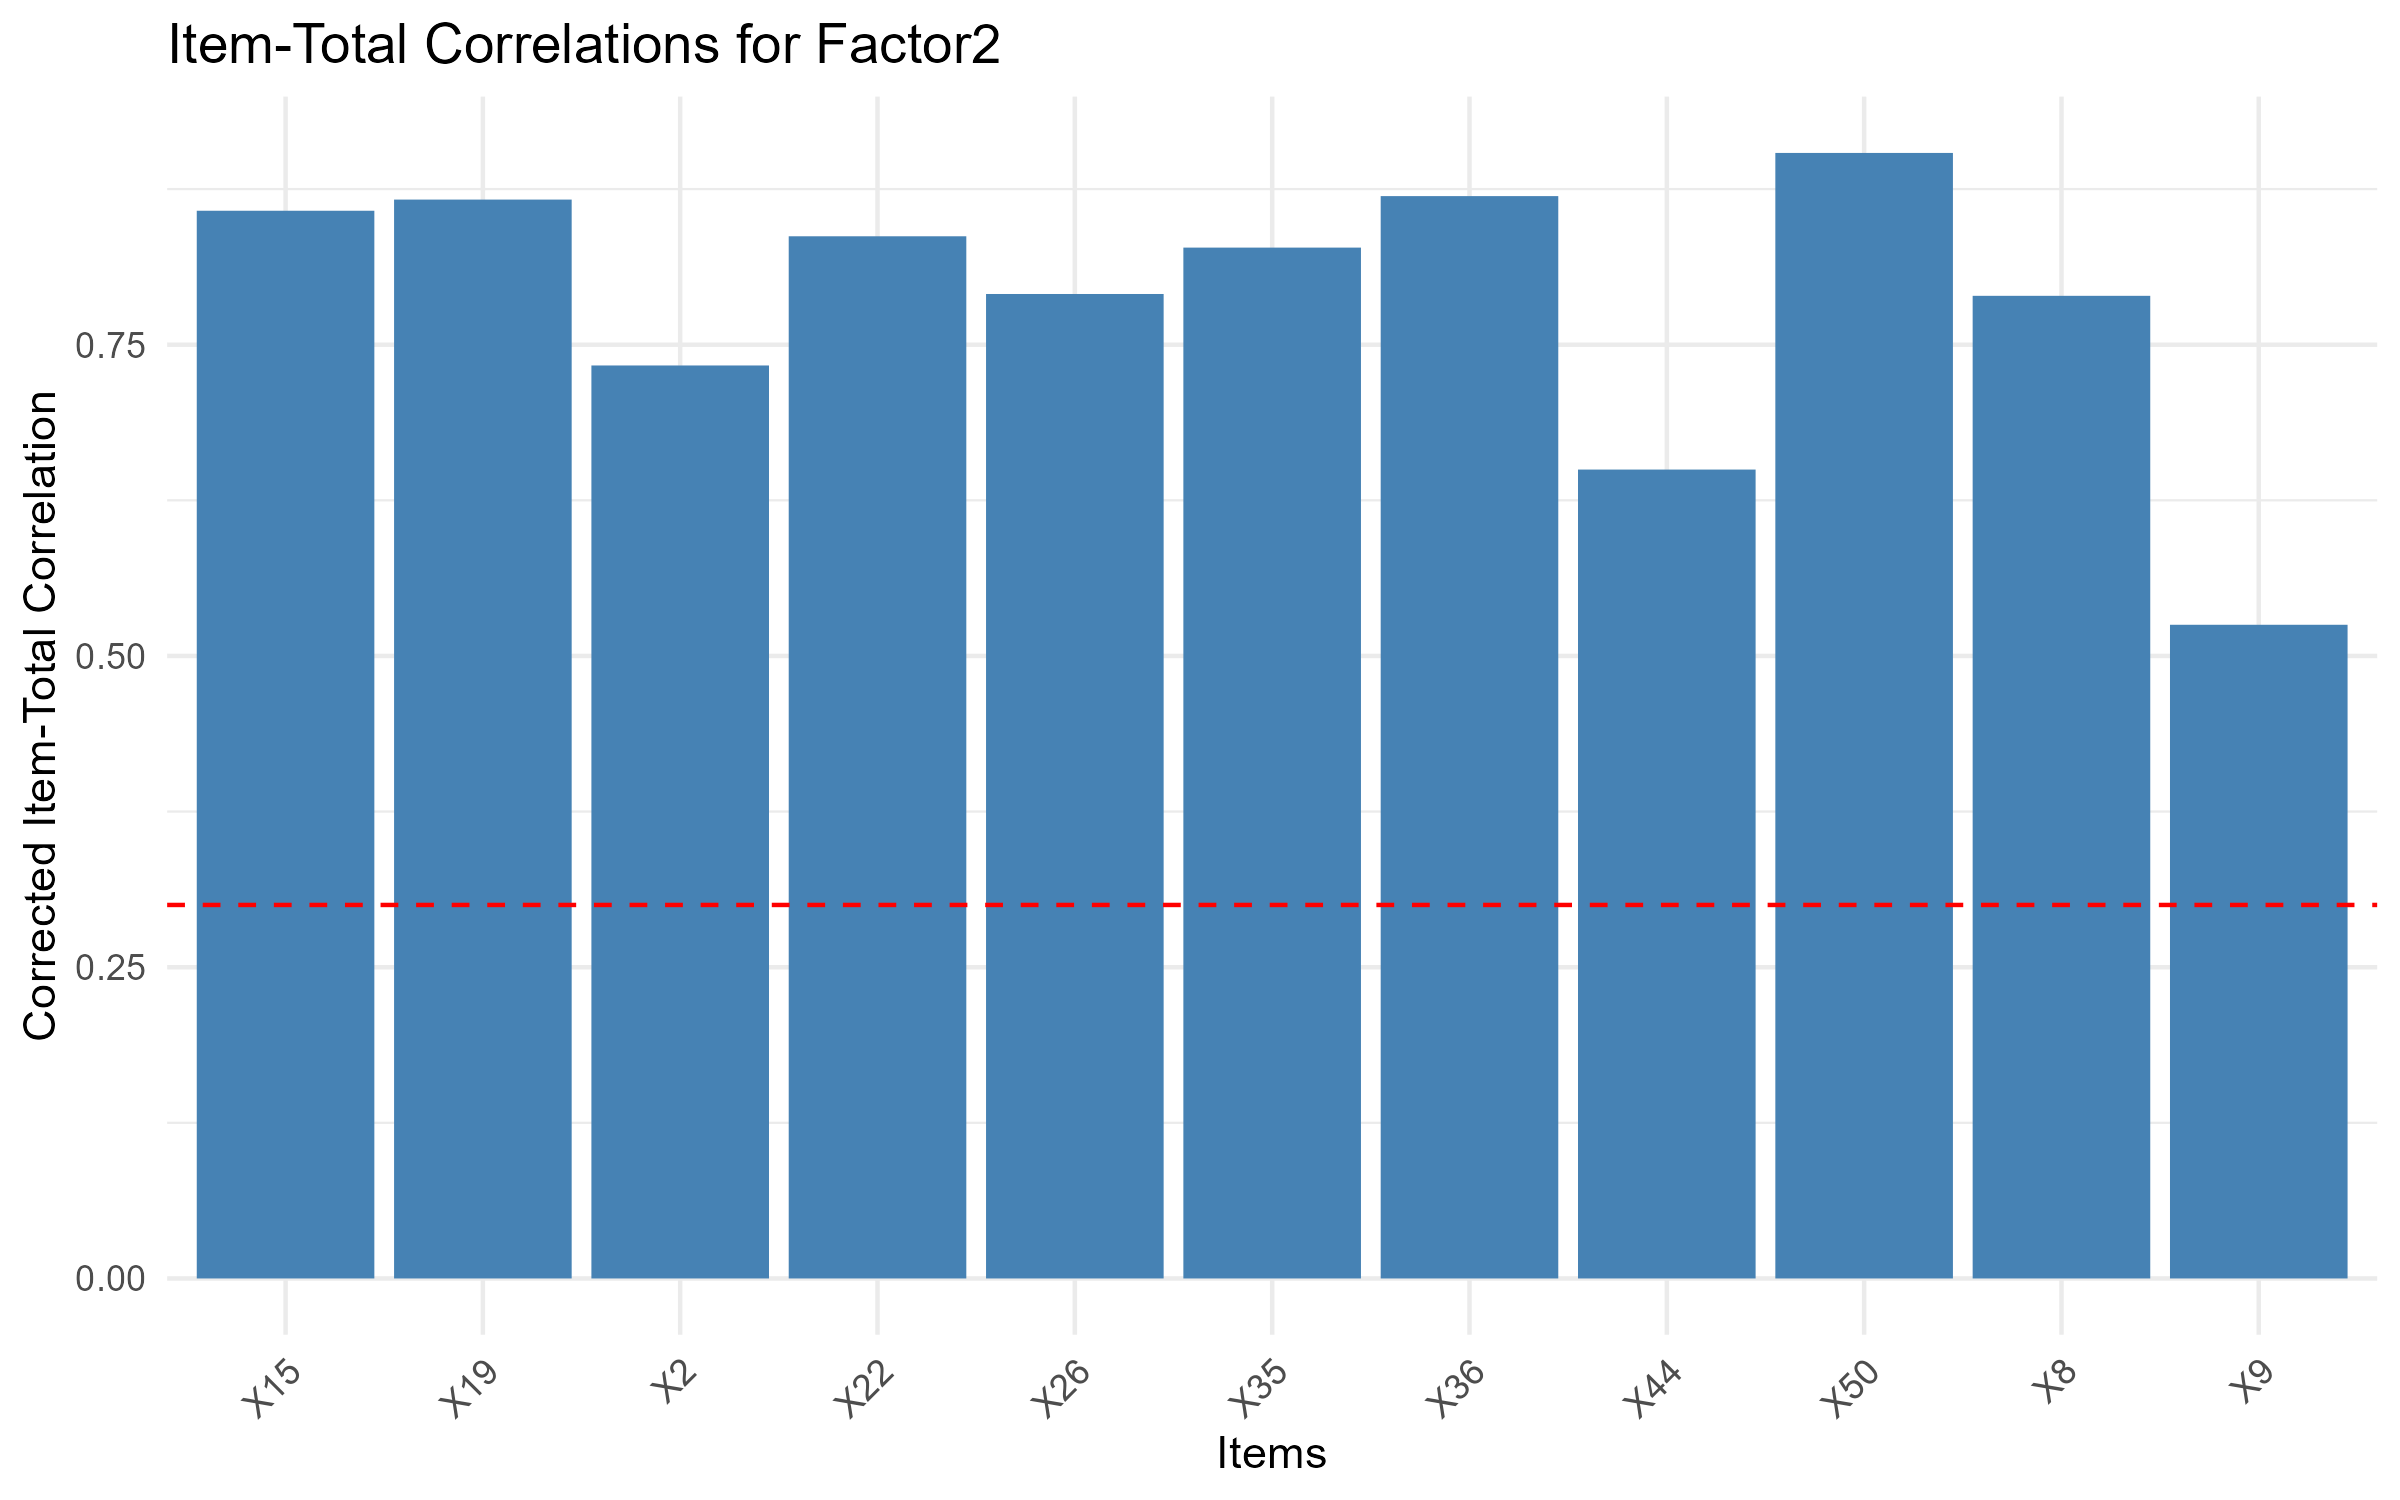
\includegraphics[width=\linewidth]{../../assets/images/reliability_Factor2.png}
        \caption{Độ tin cậy Factor 2}
        \label{fig:h3}
    \end{minipage}
    \hfill
    \begin{minipage}{0.48\textwidth}
        \centering
        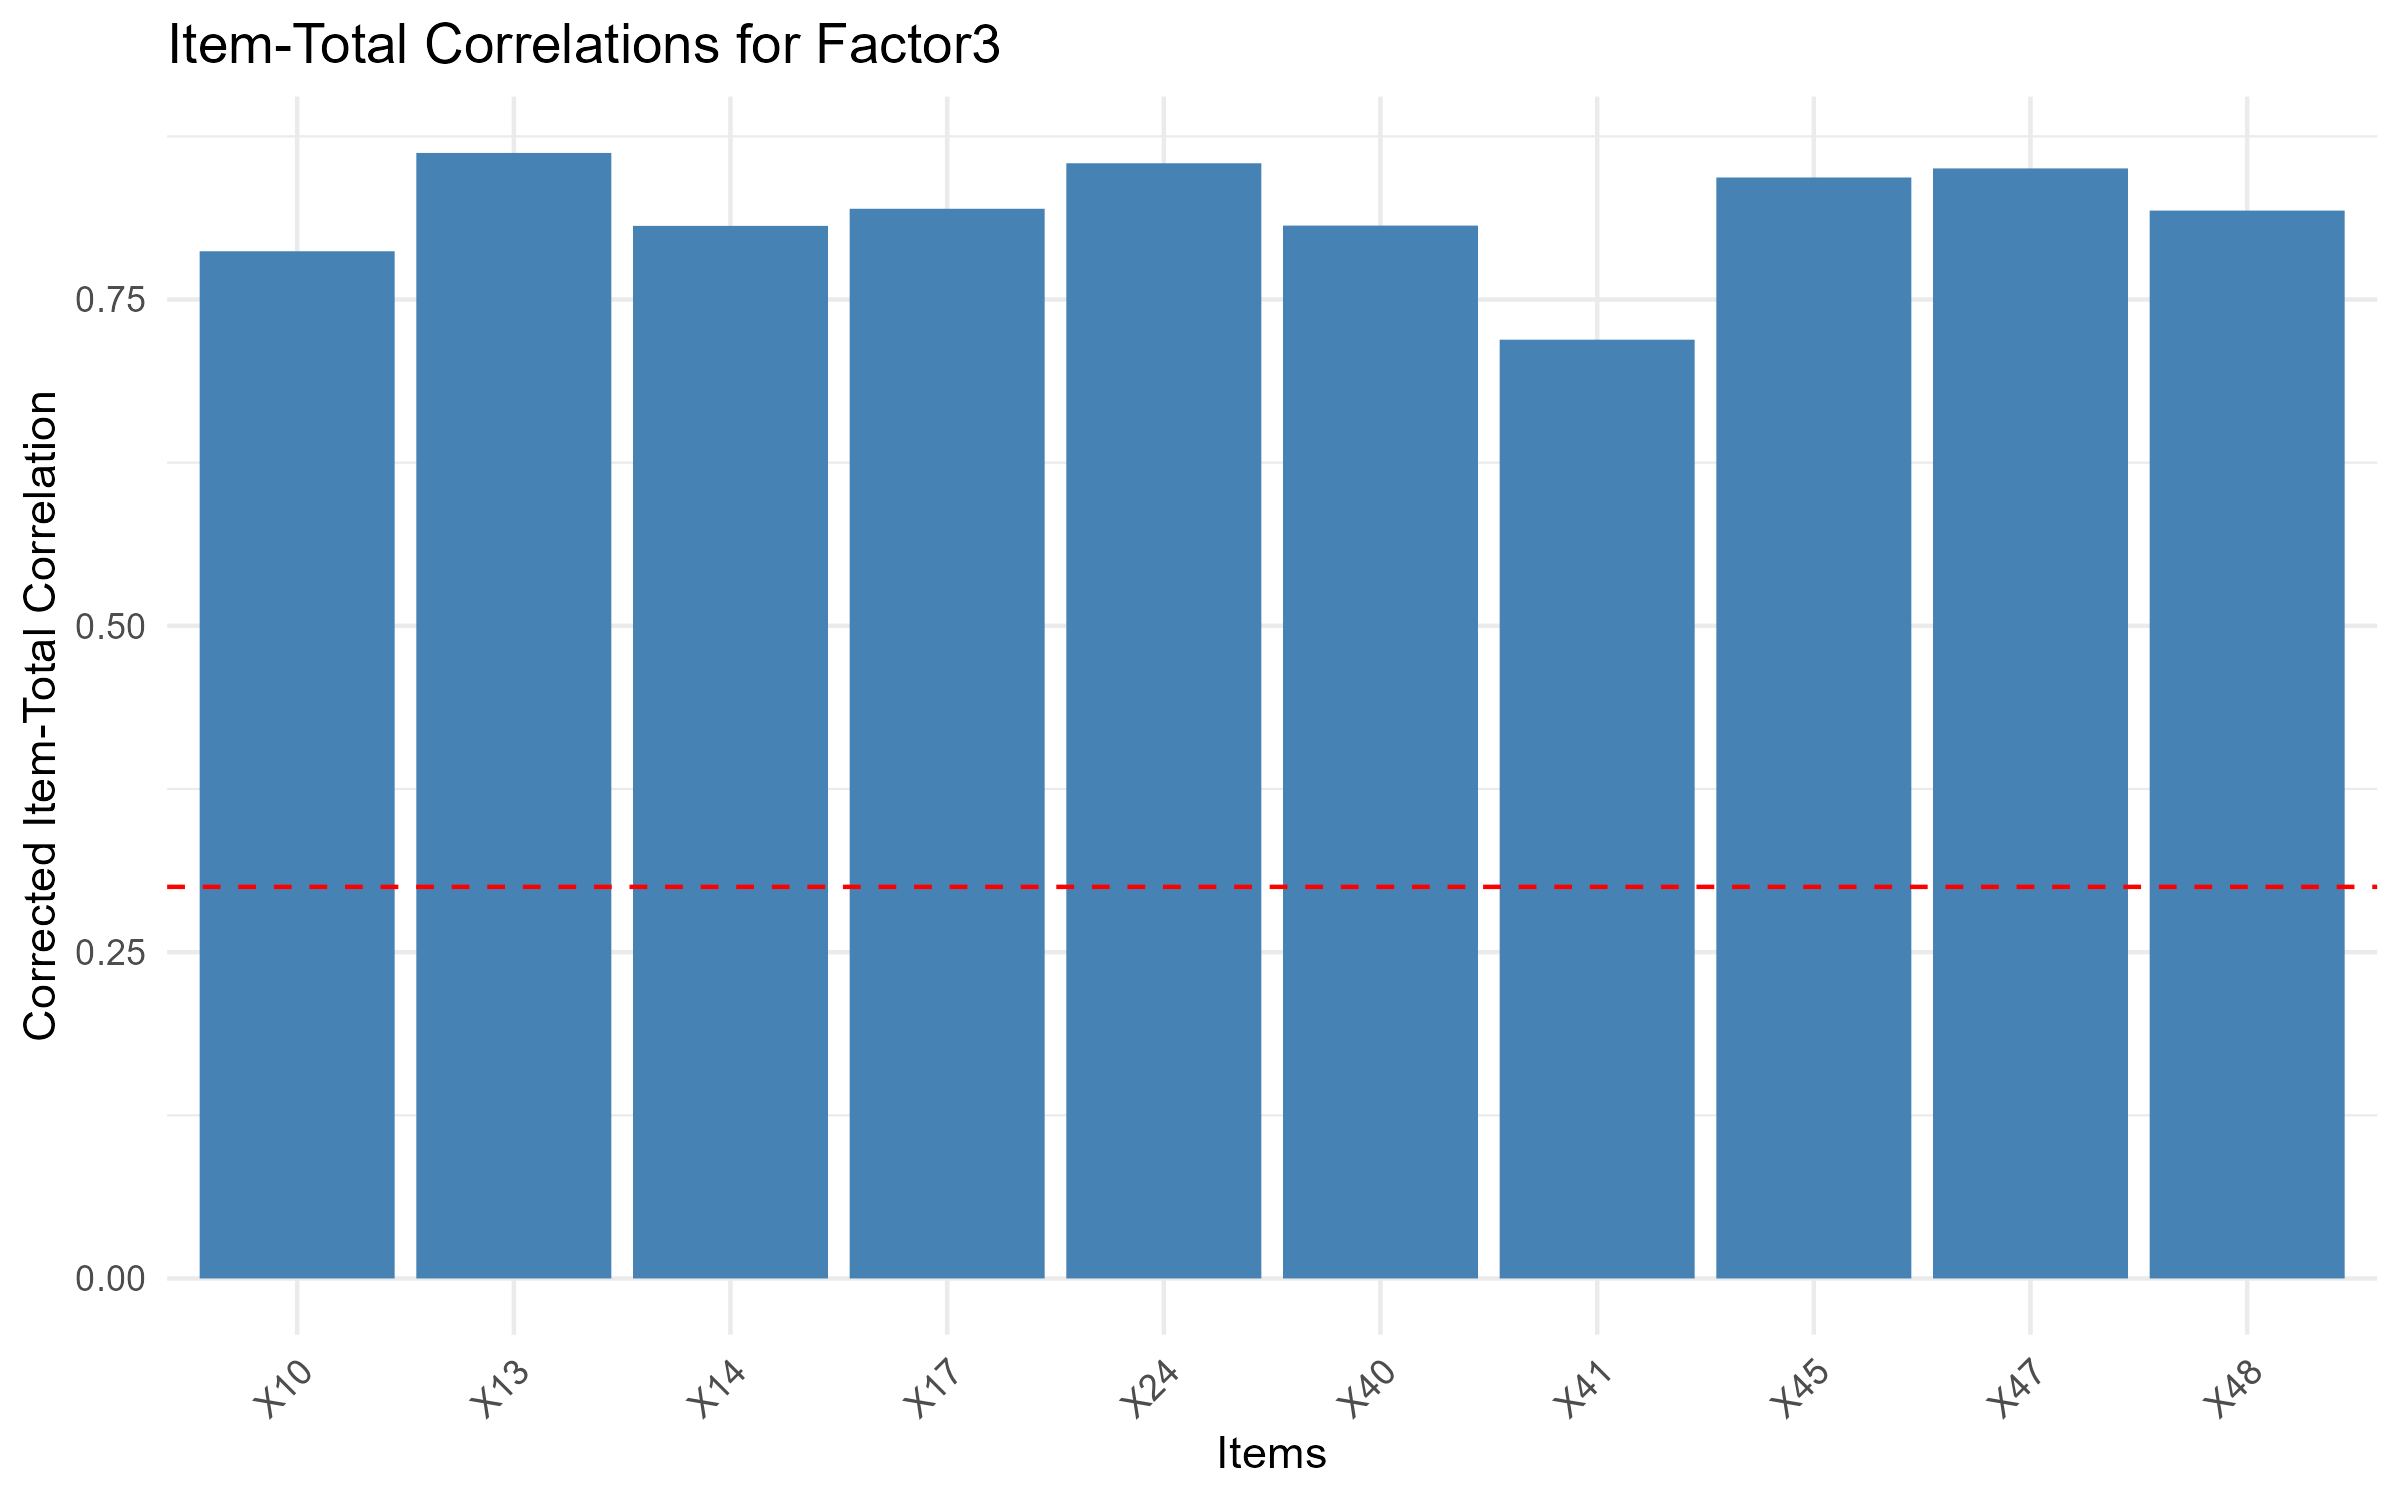
\includegraphics[width=\linewidth]{../../assets/images/reliability_Factor3.png}
        \caption{Độ tin cậy Factor 3}
        \label{fig:h4}
    \end{minipage}
\end{figure}

\begin{figure}[h!]
    \centering
    \begin{minipage}{0.48\textwidth}
        \centering
        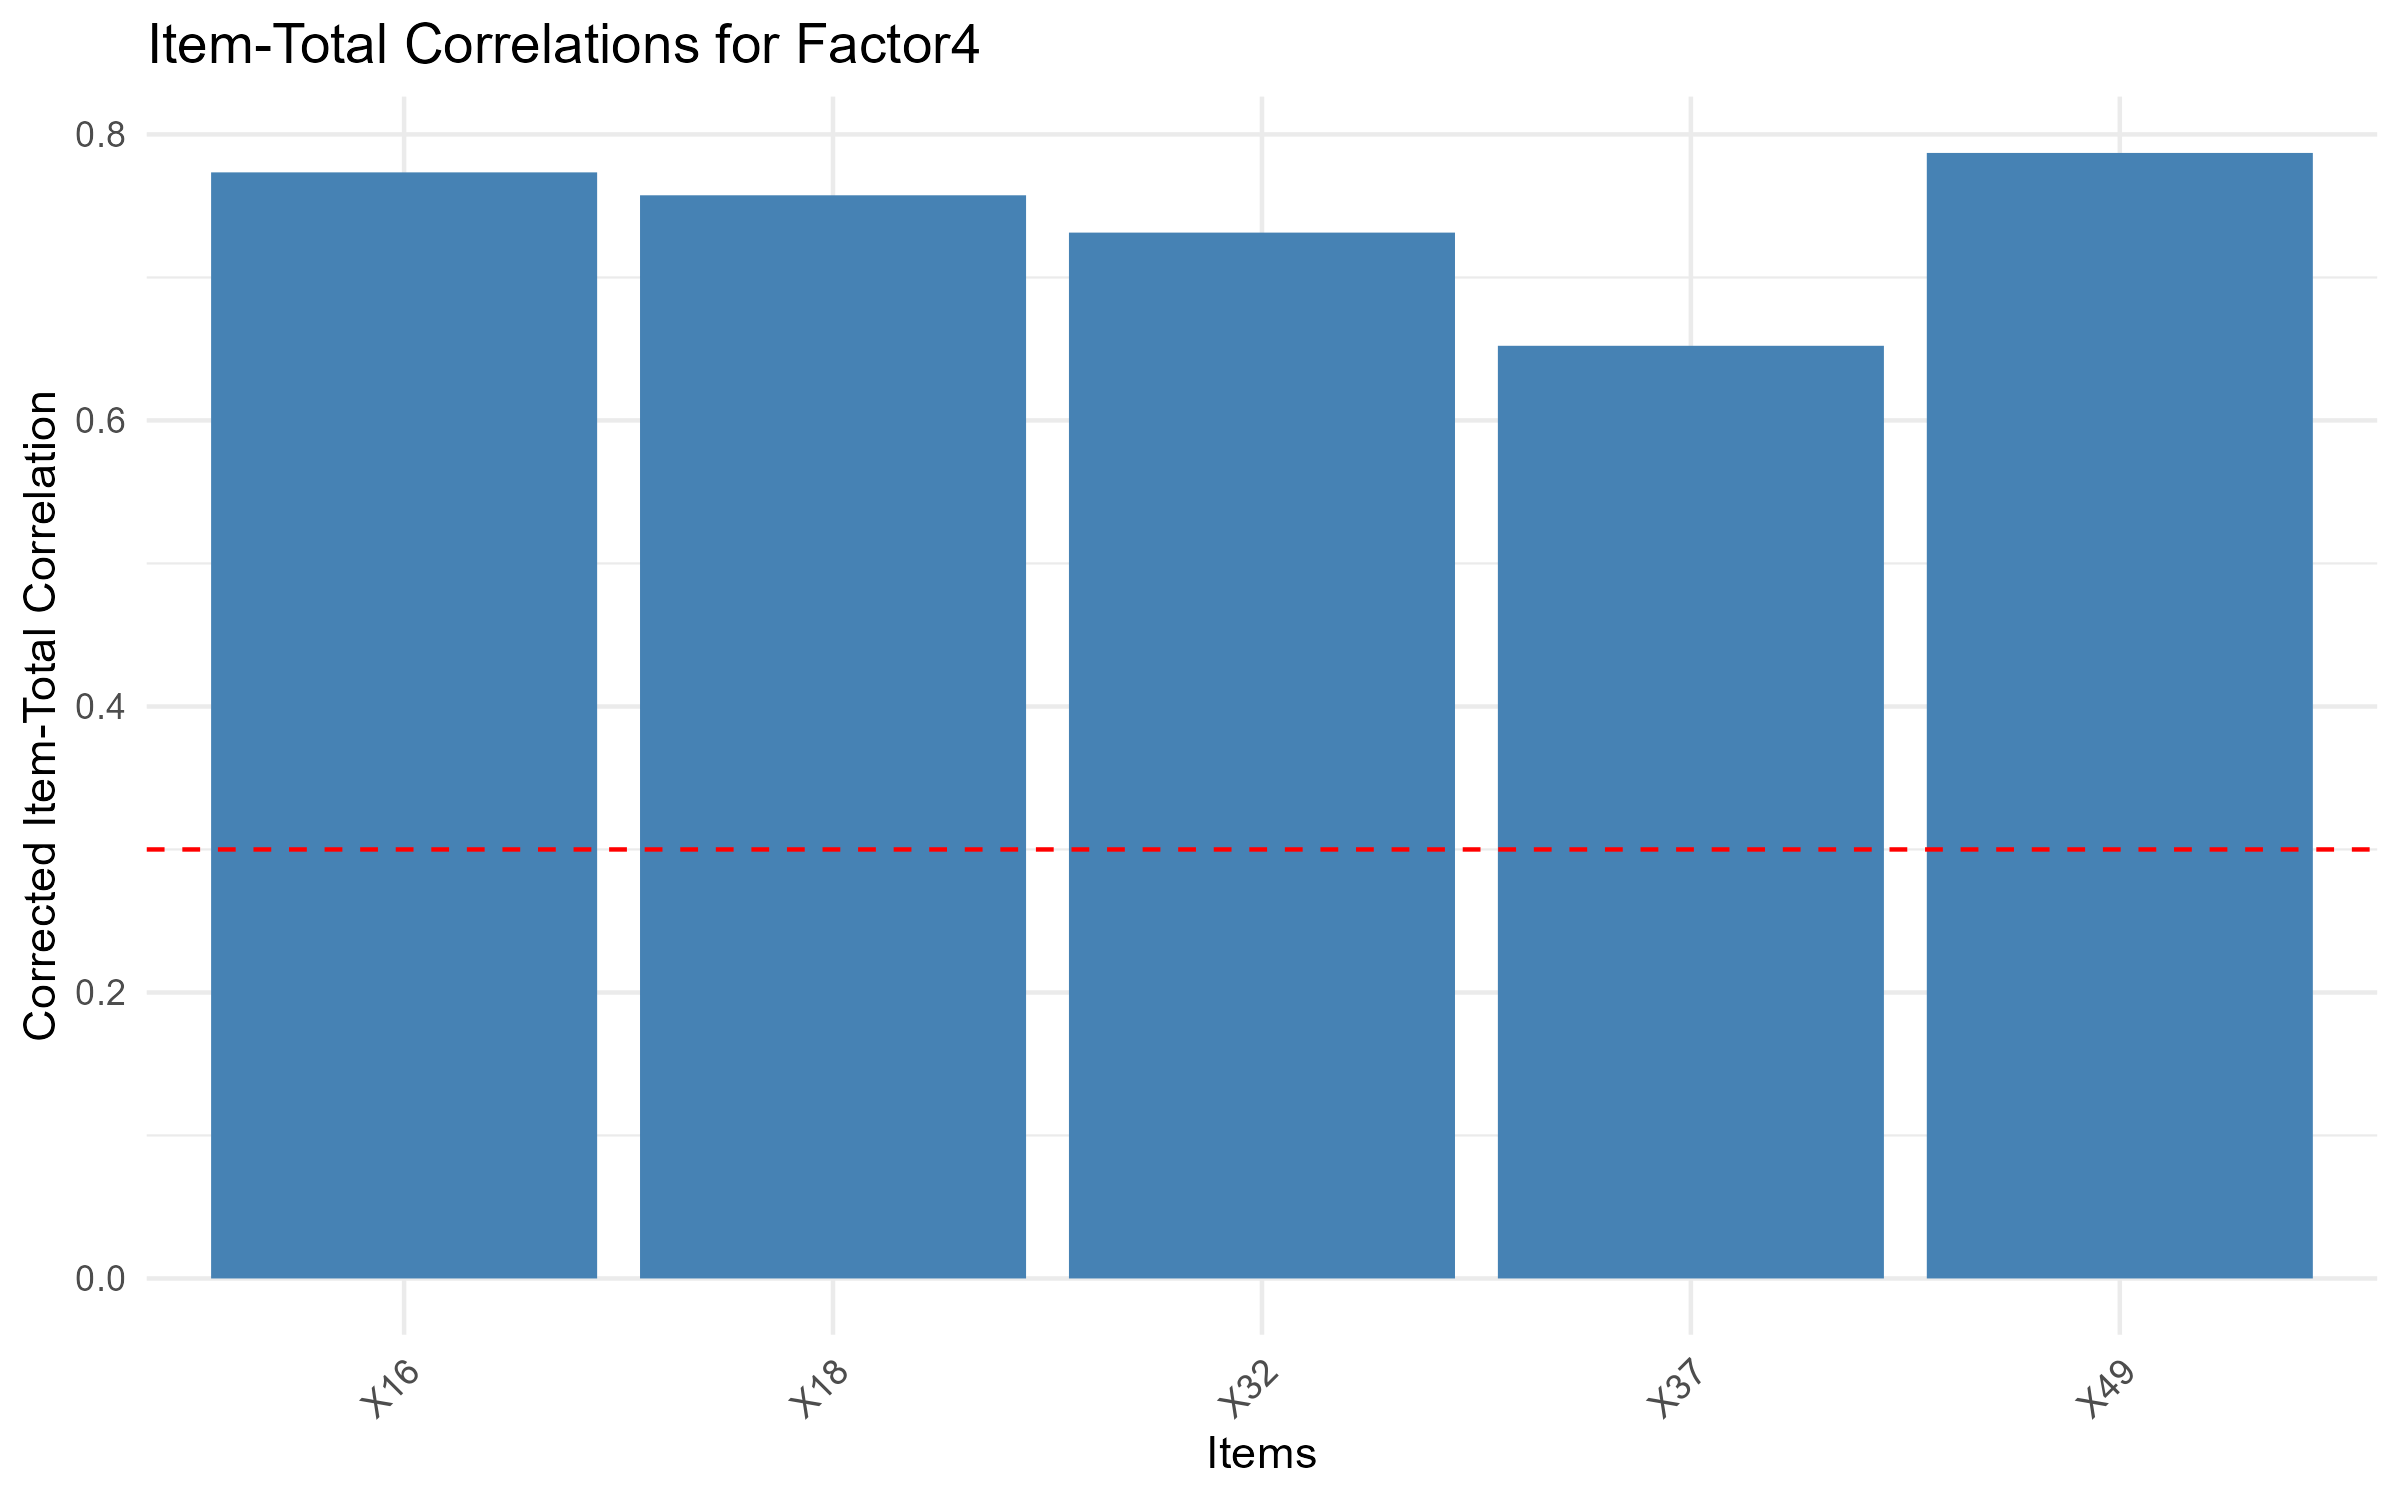
\includegraphics[width=\linewidth]{../../assets/images/reliability_Factor4.png}
        \caption{Độ tin cậy Factor 4}
        \label{fig:h5}
    \end{minipage}
    \hfill
    \begin{minipage}{0.48\textwidth}
        \centering
        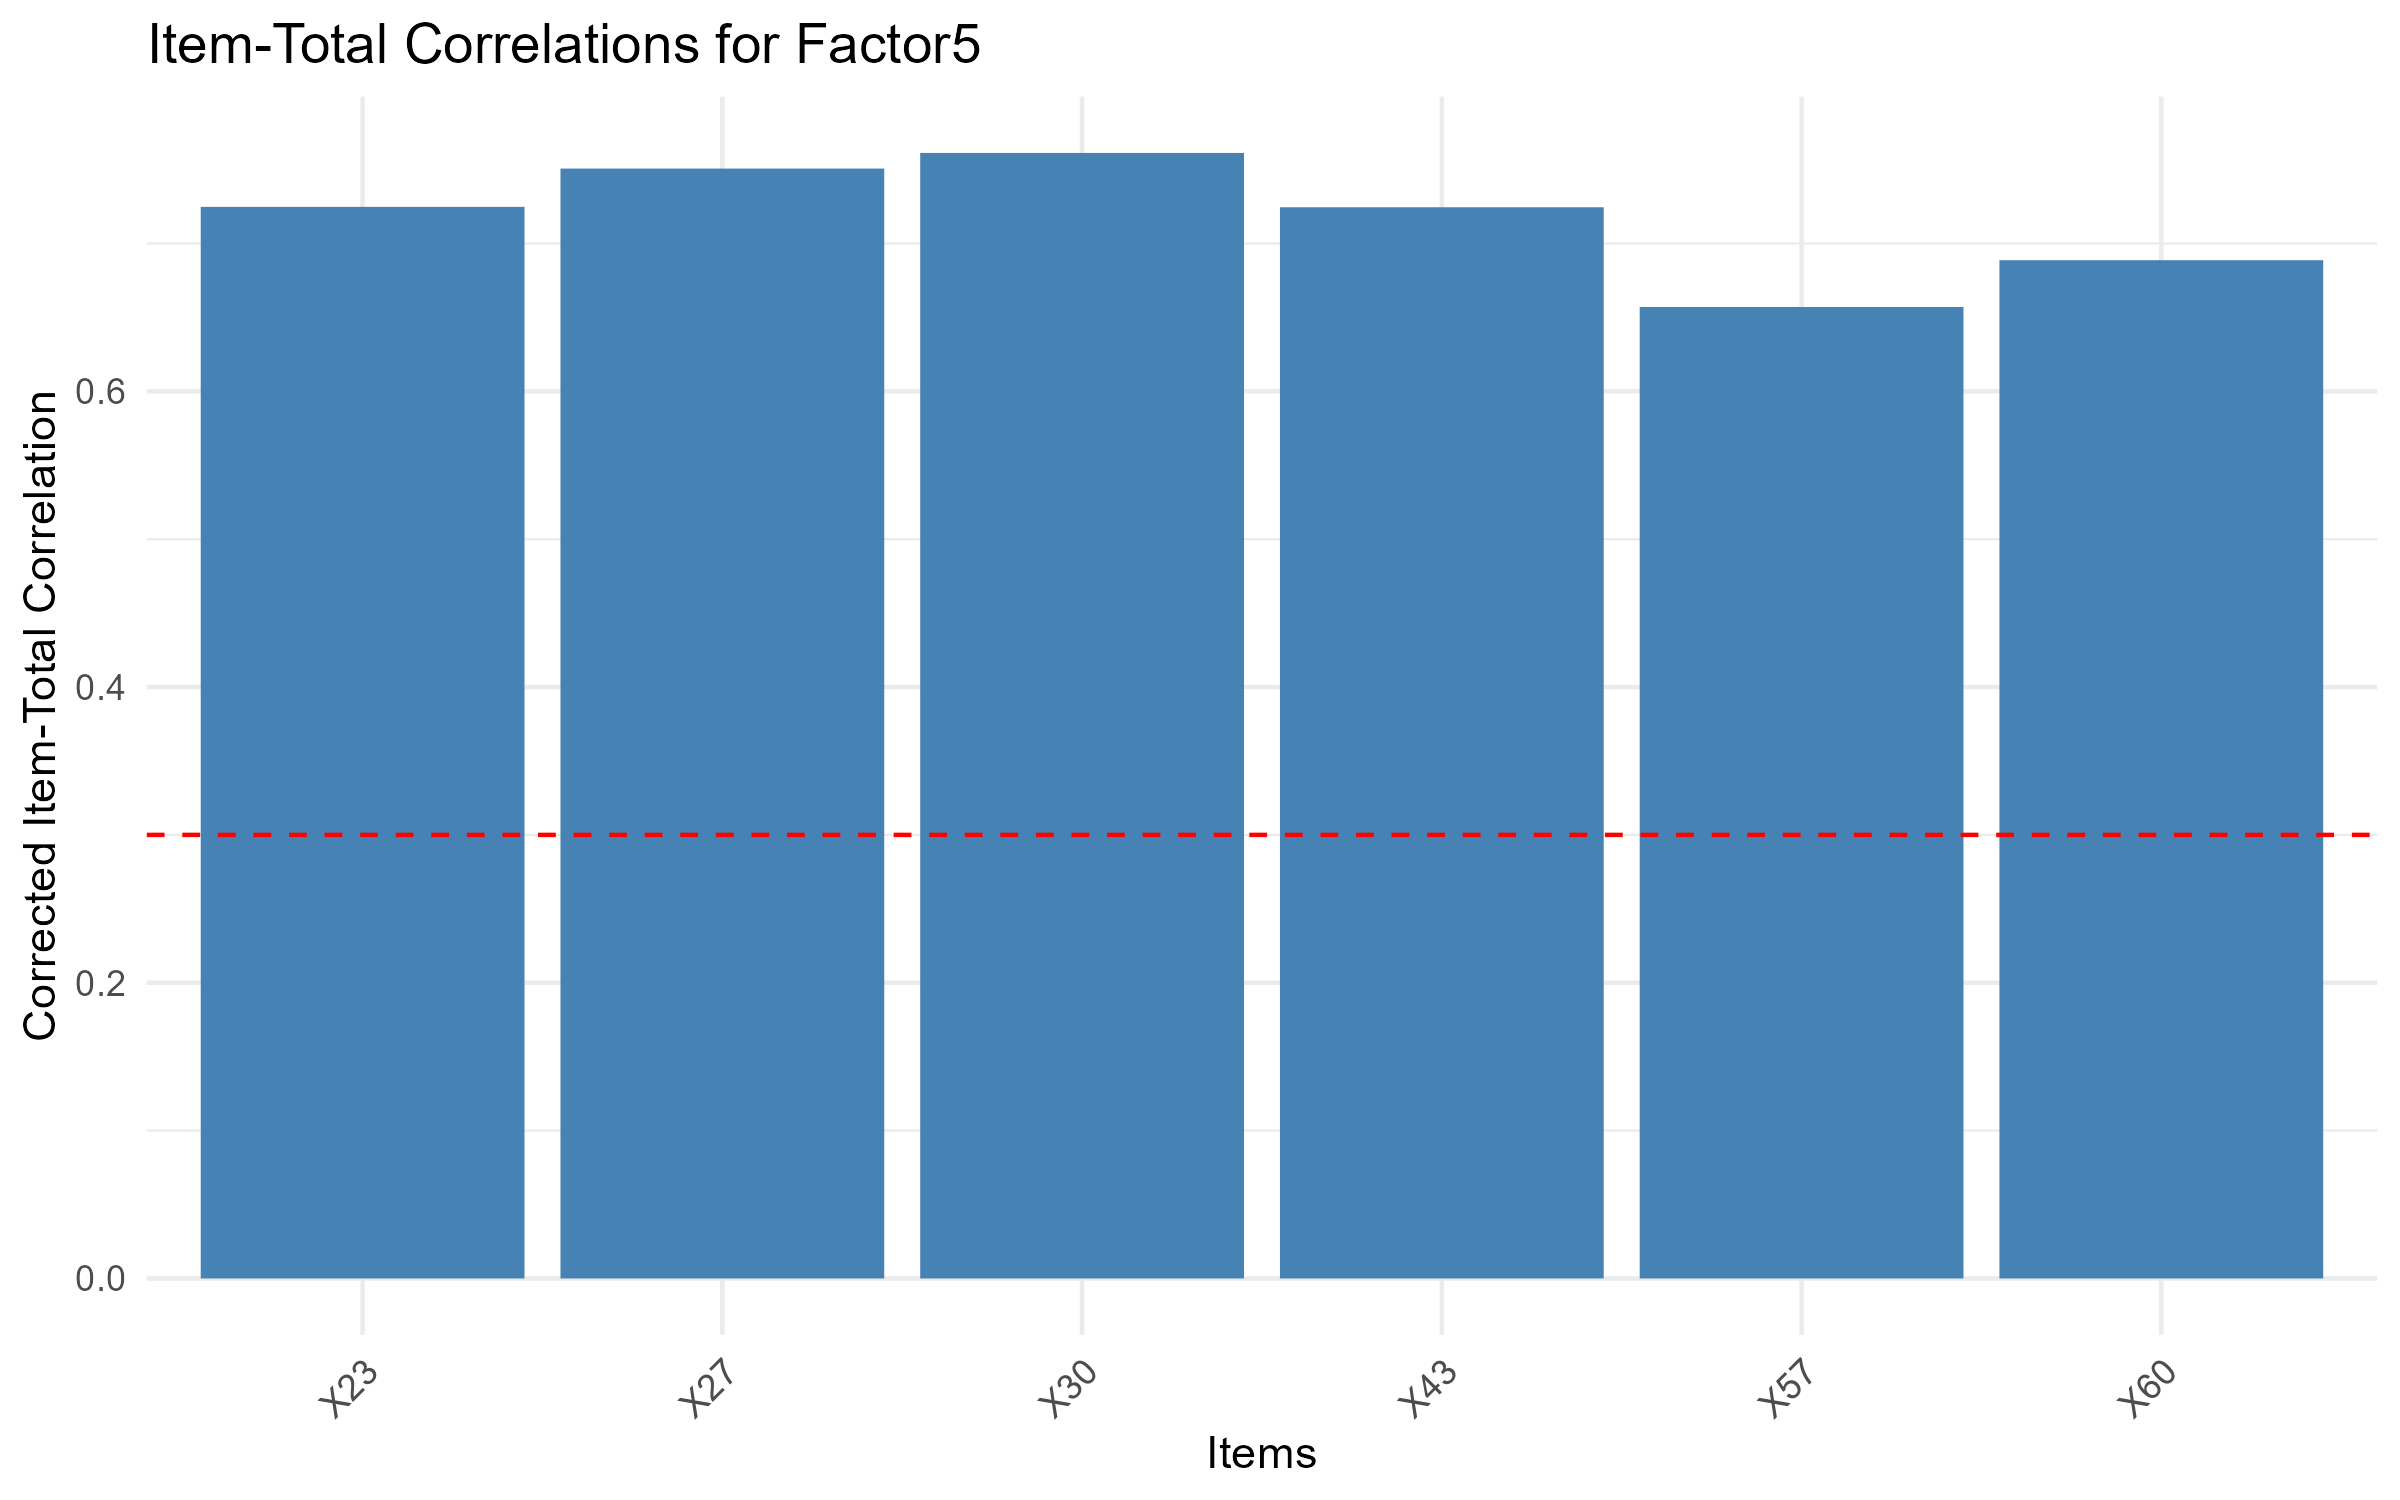
\includegraphics[width=\linewidth]{../../assets/images/reliability_Factor5.png}
        \caption{Độ tin cậy Factor 5}
        \label{fig:h6}
    \end{minipage}
\end{figure}

\begin{figure}[h!]
    \centering
    \begin{minipage}{0.48\textwidth}
        \centering
        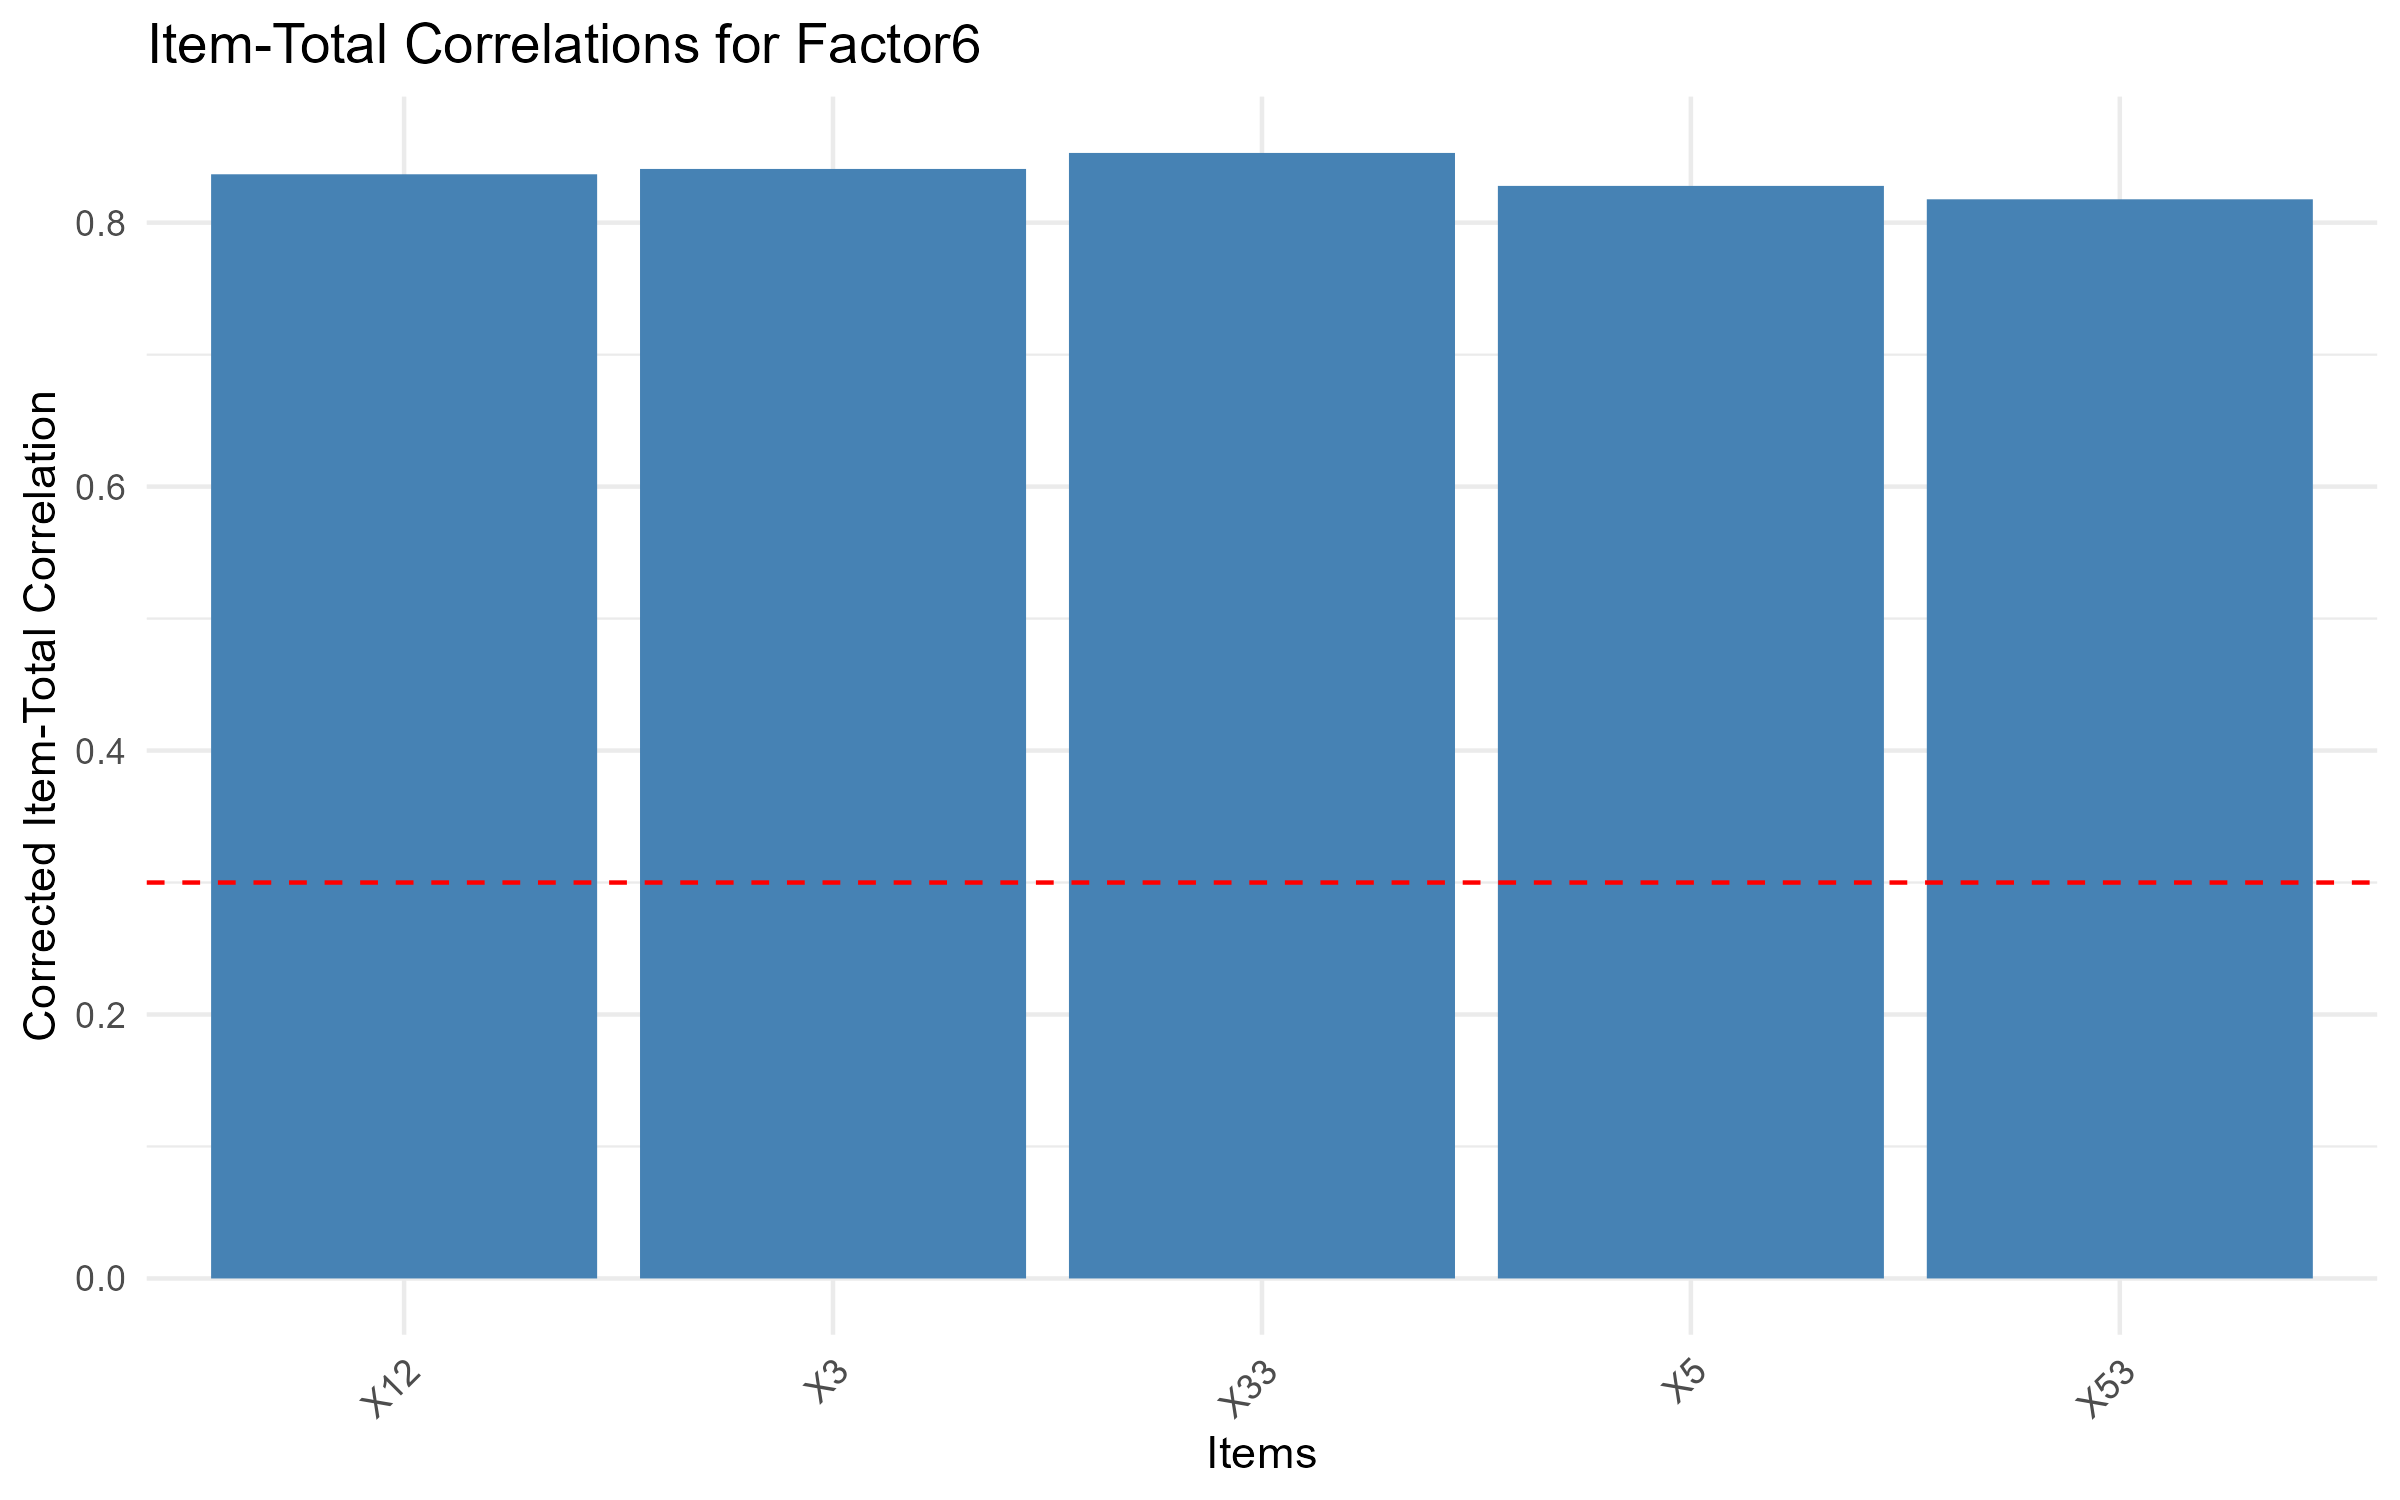
\includegraphics[width=\linewidth]{../../assets/images/reliability_Factor6.png}
        \caption{Độ tin cậy Factor 6}
        \label{fig:h7}
    \end{minipage}
    \hfill
    \begin{minipage}{0.48\textwidth}
        \centering
        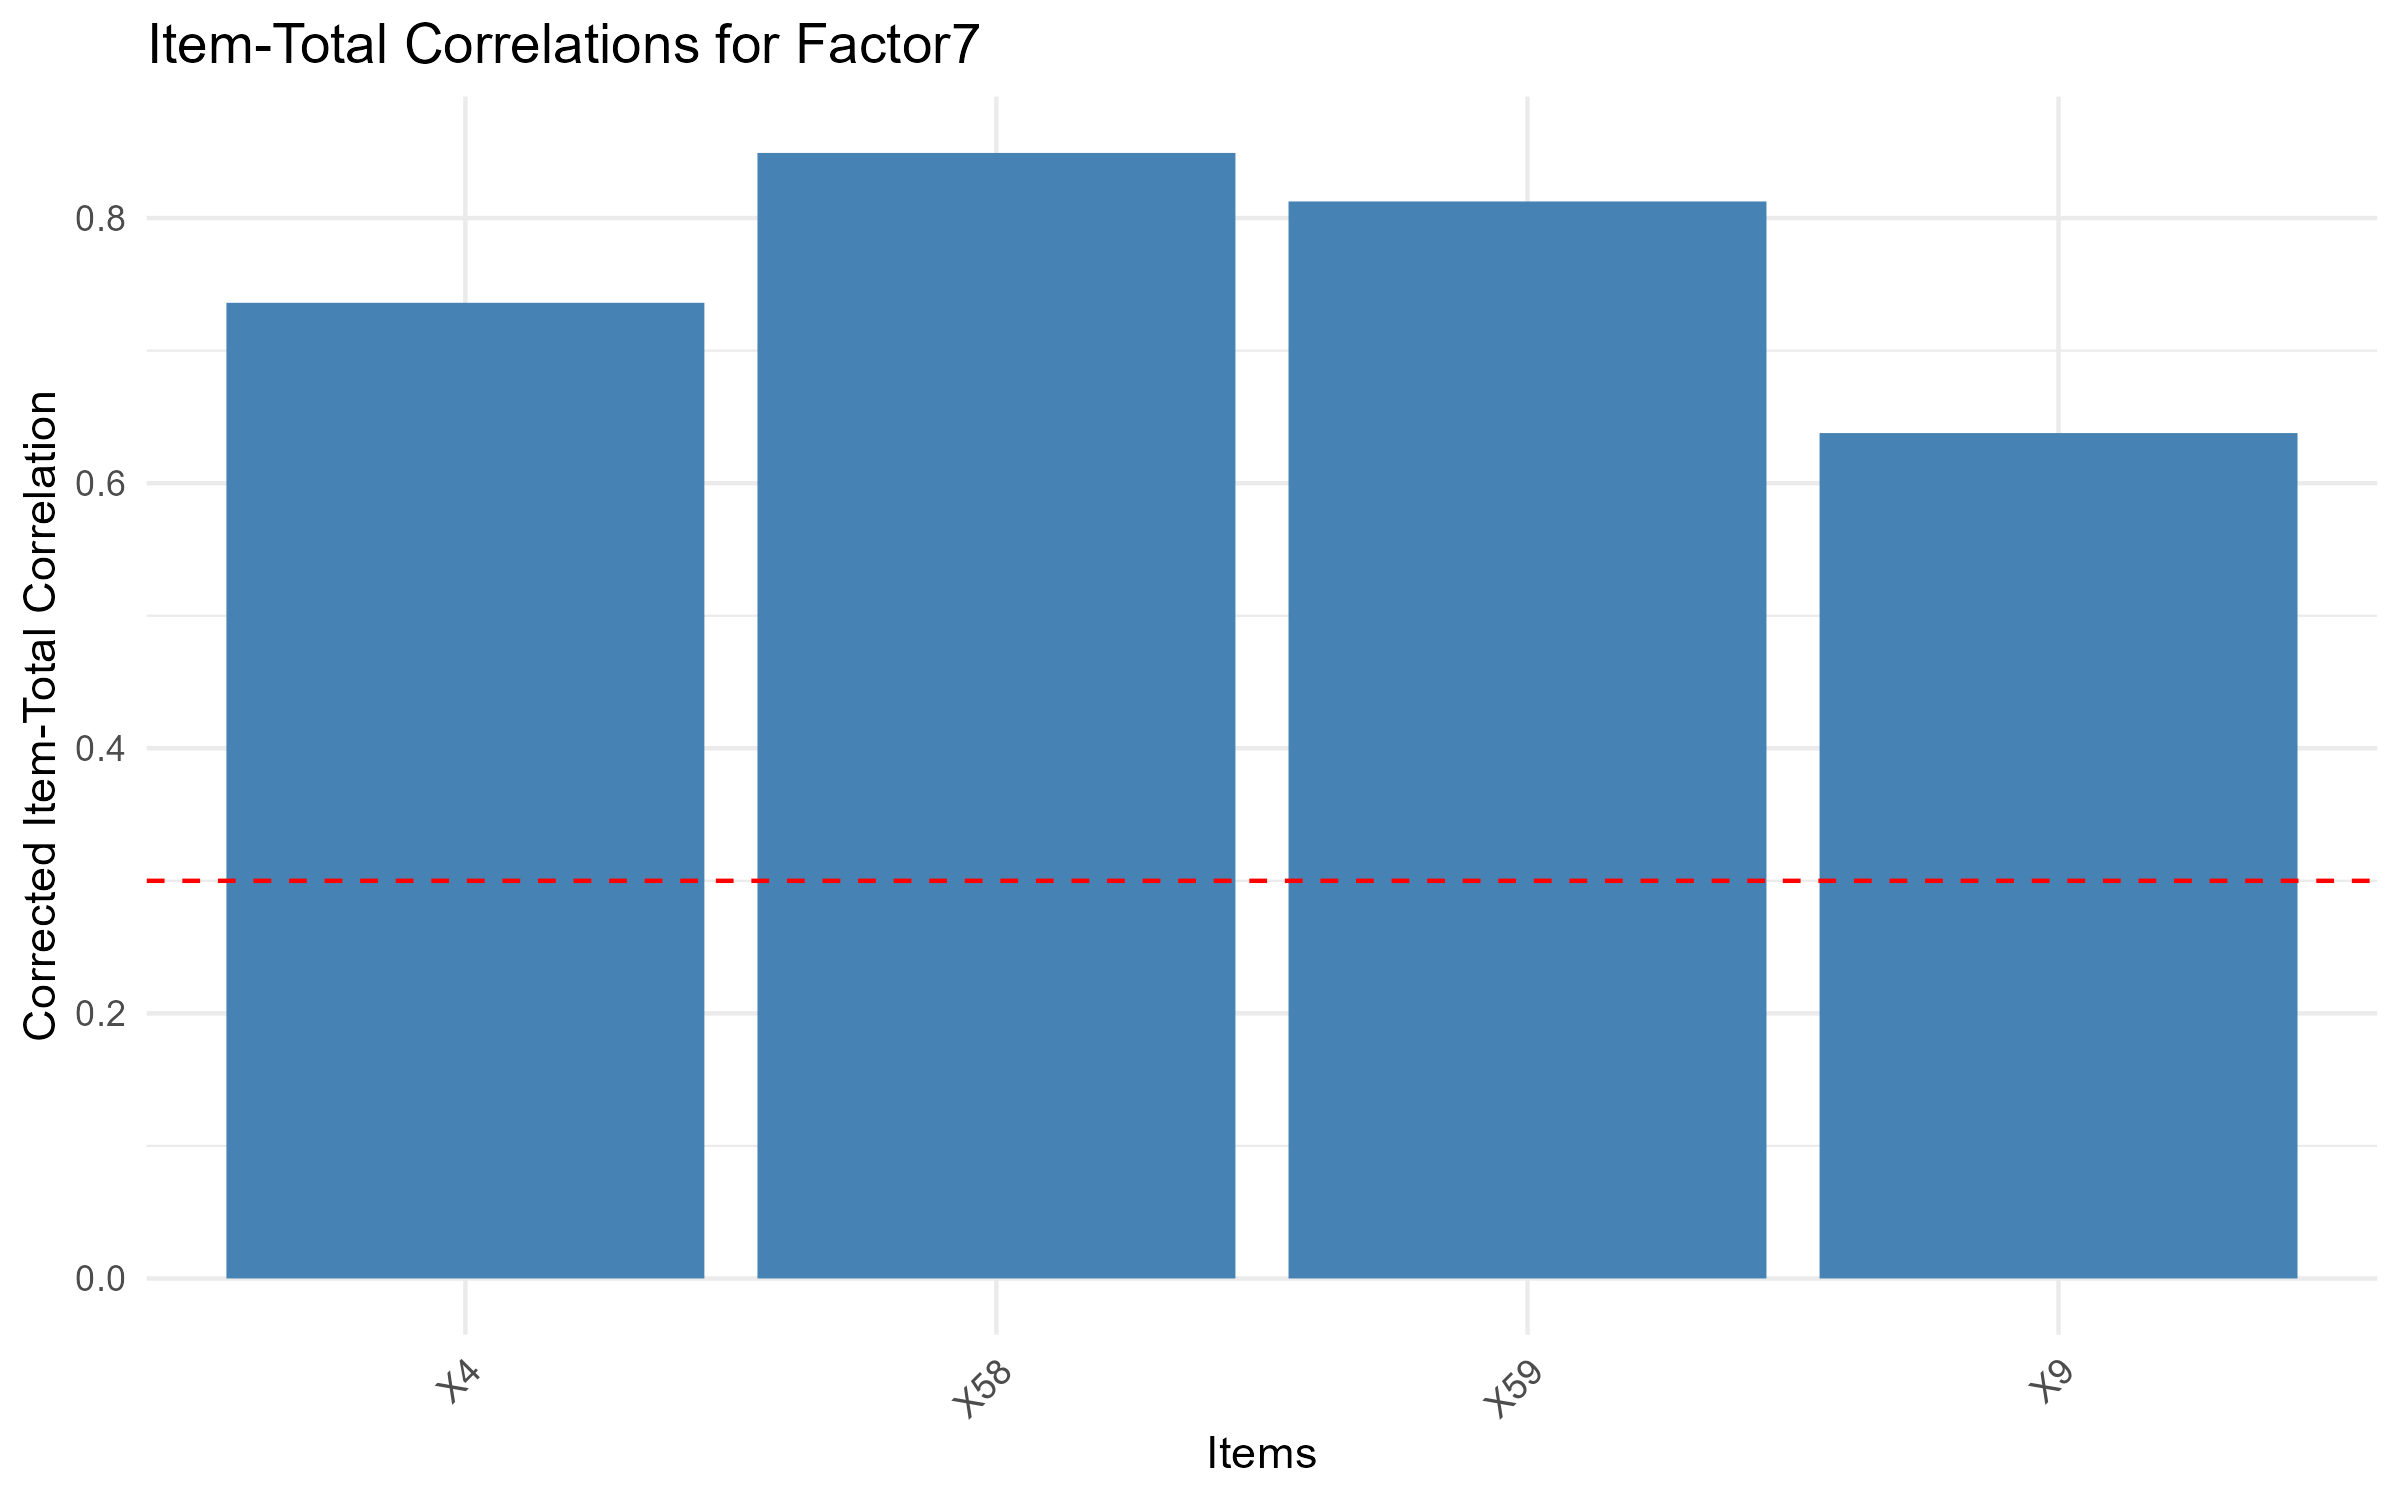
\includegraphics[width=\linewidth]{../../assets/images/reliability_Factor7.png}
        \caption{Độ tin cậy Factor 7}
        \label{fig:h8}
    \end{minipage}
\end{figure}

\subsection{Quy trình phân tích tổng hợp}

\begin{matlab}
\begin{lstlisting}
function analyze_socioeconomic_data(data, province_names, variable_names)
% Phân tích tổng hợp dữ liệu kinh tế - xã hội
% data: ma trận n x p (n tỉnh, p biến)
% province_names: tên các tỉnh
% variable_names: tên các biến

% 1. Khám phá dữ liệu
fprintf('=== THỐNG KÊ MÔ TẢ ===\n');
disp(array2table([mean(data); std(data); min(data); max(data)], ...
    'VariableNames', variable_names, ...
    'RowNames', {'Mean', 'Std', 'Min', 'Max'}));

% Ma trận tương quan
R = corrcoef(data);
figure('Name', 'Ma trận tương quan');
heatmap(variable_names, variable_names, R, ...
    'Colormap', parula, 'ColorbarVisible', 'on');
title('Ma trận tương quan giữa các biến');

% 2. Phân tích thành phần chính
fprintf('\n=== PHÂN TÍCH THÀNH PHẦN CHÍNH ===\n');
[coeff, scores, latent, ~, explained] = pca(zscore(data));

% Scree plot
figure('Name', 'PCA Results');
subplot(2,2,1);
plot(1:length(latent), latent, 'bo-', 'LineWidth', 2);
xlabel('Thành phần chính');
ylabel('Trị riêng');
title('Scree Plot');
grid on;

% Phần trăm phương sai giải thích
subplot(2,2,2);
bar(explained(1:min(5, length(explained))));
xlabel('Thành phần chính');
ylabel('Phần trăm phương sai (%)');
title('Phương sai giải thích');

% Biplot
subplot(2,2,[3,4]);
biplot(coeff(:,1:2), 'Scores', scores(:,1:2), ...
    'VarLabels', variable_names, 'ObsLabels', province_names);
xlabel(['PC1 (' num2str(explained(1), '%.1f') '%)']);
ylabel(['PC2 (' num2str(explained(2), '%.1f') '%)']);
title('Biplot PC1 vs PC2');

% In kết quả PCA
fprintf('Phần trăm phương sai giải thích:\n');
for i = 1:min(4, length(explained))
    fprintf('  PC%d: %.2f%% (tích lũy: %.2f%%)\n', ...
        i, explained(i), sum(explained(1:i)));
end

% 3. Phân tích cụm K-means
fprintf('\n=== PHÂN TÍCH CỤM ===\n');
k_range = 2:6;
silhouette_scores = zeros(size(k_range));

for i = 1:length(k_range)
    k = k_range(i);
    [idx, ~] = kmeans(zscore(data), k, 'Replicates', 10);
    silhouette_scores(i) = mean(silhouette(zscore(data), idx));
end

% Tìm số cụm tối ưu
[~, optimal_k_idx] = max(silhouette_scores);
optimal_k = k_range(optimal_k_idx);

fprintf('Số cụm tối ưu (theo Silhouette): %d\n', optimal_k);

% Phân cụm với k tối ưu
[cluster_idx, centroids] = kmeans(zscore(data), optimal_k, 'Replicates', 20);

% Hiển thị kết quả phân cụm
figure('Name', 'Clustering Results');
subplot(1,2,1);
plot(k_range, silhouette_scores, 'bo-', 'LineWidth', 2);
xlabel('Số cụm');
ylabel('Silhouette Score');
title('Lựa chọn số cụm');
grid on;

subplot(1,2,2);
gscatter(scores(:,1), scores(:,2), cluster_idx);
xlabel(['PC1 (' num2str(explained(1), '%.1f') '%)']);
ylabel(['PC2 (' num2str(explained(2), '%.1f') '%)']);
title(['Kết quả phân cụm (k=' num2str(optimal_k) ')']);
legend('Location', 'best');

% In danh sách từng cụm
for c = 1:optimal_k
    fprintf('\nCụm %d (%d tỉnh):\n', c, sum(cluster_idx == c));
    cluster_provinces = province_names(cluster_idx == c);
    for j = 1:length(cluster_provinces)
        fprintf('  %s\n', cluster_provinces{j});
    end
end

% 4. Đặc trưng từng cụm
fprintf('\n=== ĐặC TRƯNG CÁC CỤM ===\n');
for c = 1:optimal_k
    fprintf('\nCụm %d:\n', c);
    cluster_data = data(cluster_idx == c, :);
    cluster_means = mean(cluster_data);
    
    for v = 1:length(variable_names)
        fprintf('  %s: %.2f ± %.2f\n', variable_names{v}, ...
            cluster_means(v), std(cluster_data(:,v)));
    end
end

end
\end{lstlisting}
\end{matlab}

\subsection{Đánh giá hiệu quả mô hình}
\subsubsection*{Cross-validation cho PCA}
Đánh giá tính ổn định của các thành phần chính thông qua validation chéo.

\subsubsection*{Metrics cho clustering}
\begin{itemize}
    \item \textbf{Silhouette coefficient}: $s_i = \frac{b_i - a_i}{\max(a_i, b_i)}$
    \item \textbf{Calinski-Harabasz index}: $\frac{SS_B/(k-1)}{SS_W/(n-k)}$
    \item \textbf{Davies-Bouldin index}: $\frac{1}{k}\sum_{i=1}^k \max_{j \neq i} \frac{\sigma_i + \sigma_j}{d_{ij}}$
\end{itemize}

\noindent % Để loại bỏ thụt lề đầu dòng
\begin{minipage}{0.4\textwidth} % Phần hình ảnh (40% chiều rộng trang)
    \centering
    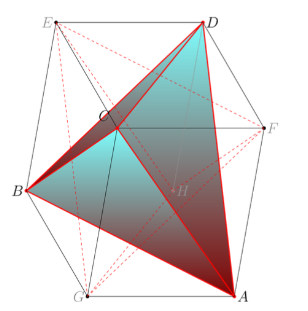
\includegraphics[width=\textwidth]{../../assets/images/figure-1.png} % Đường dẫn tới ảnh
    \captionof{figure}{Quy trình phân tích dữ liệu nhiều chiều} % Chú thích cho hình
    \label{fig:multivariate_workflow}
\end{minipage}%
\hfill % Thêm khoảng cách giữa hình và chữ
\begin{minipage}{0.55\textwidth} % Phần văn bản (55% chiều rộng trang)
    Quy trình phân tích dữ liệu nhiều chiều tổng hợp bao gồm nhiều bước từ khám phá dữ liệu ban đầu đến xây dựng mô hình cuối cùng. Mỗi kỹ thuật có ưu điểm riêng và cần được lựa chọn phù hợp với mục tiêu nghiên cứu cụ thể. Việc kết hợp nhiều phương pháp thường cho kết quả toàn diện và đáng tin cậy hơn.
\end{minipage}

\section{Phân tích nhân tố khám phá (EFA)}

EFA là một kỹ thuật thống kê được sử dụng để xác định cấu trúc ẩn trong một tập dữ liệu với nhiều biến quan sát \cite{vu2022, hair2019, tabachnick2019}.

\subsection{Mô hình phân tích nhân tố}

\begin{matlab}
\begin{lstlisting}
function [loadings, eigenvals, explained_var, rotated_loadings] = ...
    exploratory_factor_analysis(data, n_factors, rotation_method)
% EXPLORATORY_FACTOR_ANALYSIS
% Thực hiện phân tích nhân tố khám phá với xoay nhân tố

% Chuẩn hóa dữ liệu
data_std = zscore(data);

% Tính ma trận tương quan
R = corr(data_std);

% Phân tích thành phần chính
[coeff, ~, eigenvals] = pca(data_std);

% Trích n_factors nhân tố đầu tiên
loadings = coeff(:, 1:n_factors) * diag(sqrt(eigenvals(1:n_factors)));

% Tính phần trăm phương sai giải thích
total_var = sum(eigenvals);
explained_var = 100 * eigenvals(1:n_factors) / total_var;

% Xoay nhân tố
switch lower(rotation_method)
    case 'varimax'
        [rotated_loadings, T] = rotatefactors(loadings, 'Method', 'varimax');
    case 'quartimax'
        [rotated_loadings, T] = rotatefactors(loadings, 'Method', 'quartimax');
    otherwise
        rotated_loadings = loadings;
        T = eye(n_factors);
end

% Hiển thị kết quả
fprintf('=== PHÂN TÍCH NHÂN TỐ KHÁM PHÁ ===\n');
fprintf('Số nhân tố: %d\n', n_factors);
fprintf('Phương pháp xoay: %s\n', rotation_method);

communalities = sum(rotated_loadings.^2, 2);
fprintf('\nCommunalities trung bình: %.3f\n', mean(communalities));
end
\end{lstlisting}
\end{matlab}

\begin{figure}[h!]
    \centering
    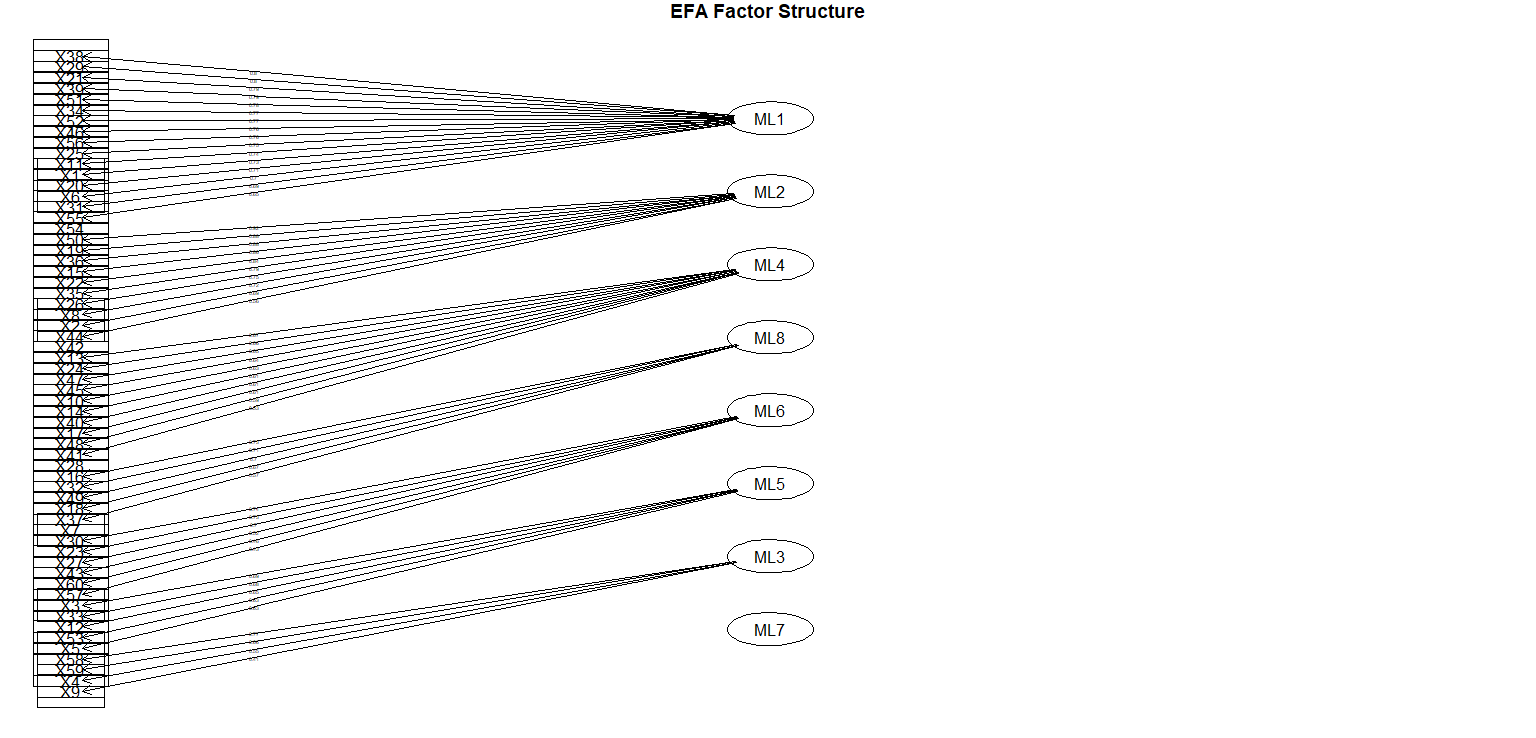
\includegraphics[width=0.8\linewidth]{../../assets/images/EFA_ML.png}
    \caption{Kết quả phân tích nhân tố khám phá với phương pháp Maximum Likelihood}
\end{figure}

\subsection{Kiểm định độ tin cậy Cronbach's Alpha}

\begin{matlab}
\begin{lstlisting}
function alpha = cronbach_alpha(X)
% CRONBACH_ALPHA - Tính hệ số tin cậy Cronbach's Alpha
%
% INPUT: X - ma trận dữ liệu (n x k), k là số biến
% OUTPUT: alpha - hệ số Cronbach's Alpha

[n, k] = size(X);

% Tính phương sai của từng biến
var_items = var(X, 1);

% Tính phương sai của tổng điểm
total_score = sum(X, 2);
var_total = var(total_score, 1);

% Tính Cronbach's Alpha
alpha = (k / (k - 1)) * (1 - sum(var_items) / var_total);

fprintf('Cronbach Alpha = %.4f\n', alpha);
if alpha >= 0.9
    fprintf('Độ tin cậy: Tuyệt vời\n');
elseif alpha >= 0.8
    fprintf('Độ tin cậy: Tốt\n');
elseif alpha >= 0.7
    fprintf('Độ tin cậy: Chấp nhận được\n');
else
    fprintf('Độ tin cậy: Kém\n');
end
end
\end{lstlisting}
\end{matlab}

\begin{figure}[h!]
    \centering
    \begin{minipage}{0.45\textwidth}
        \centering
        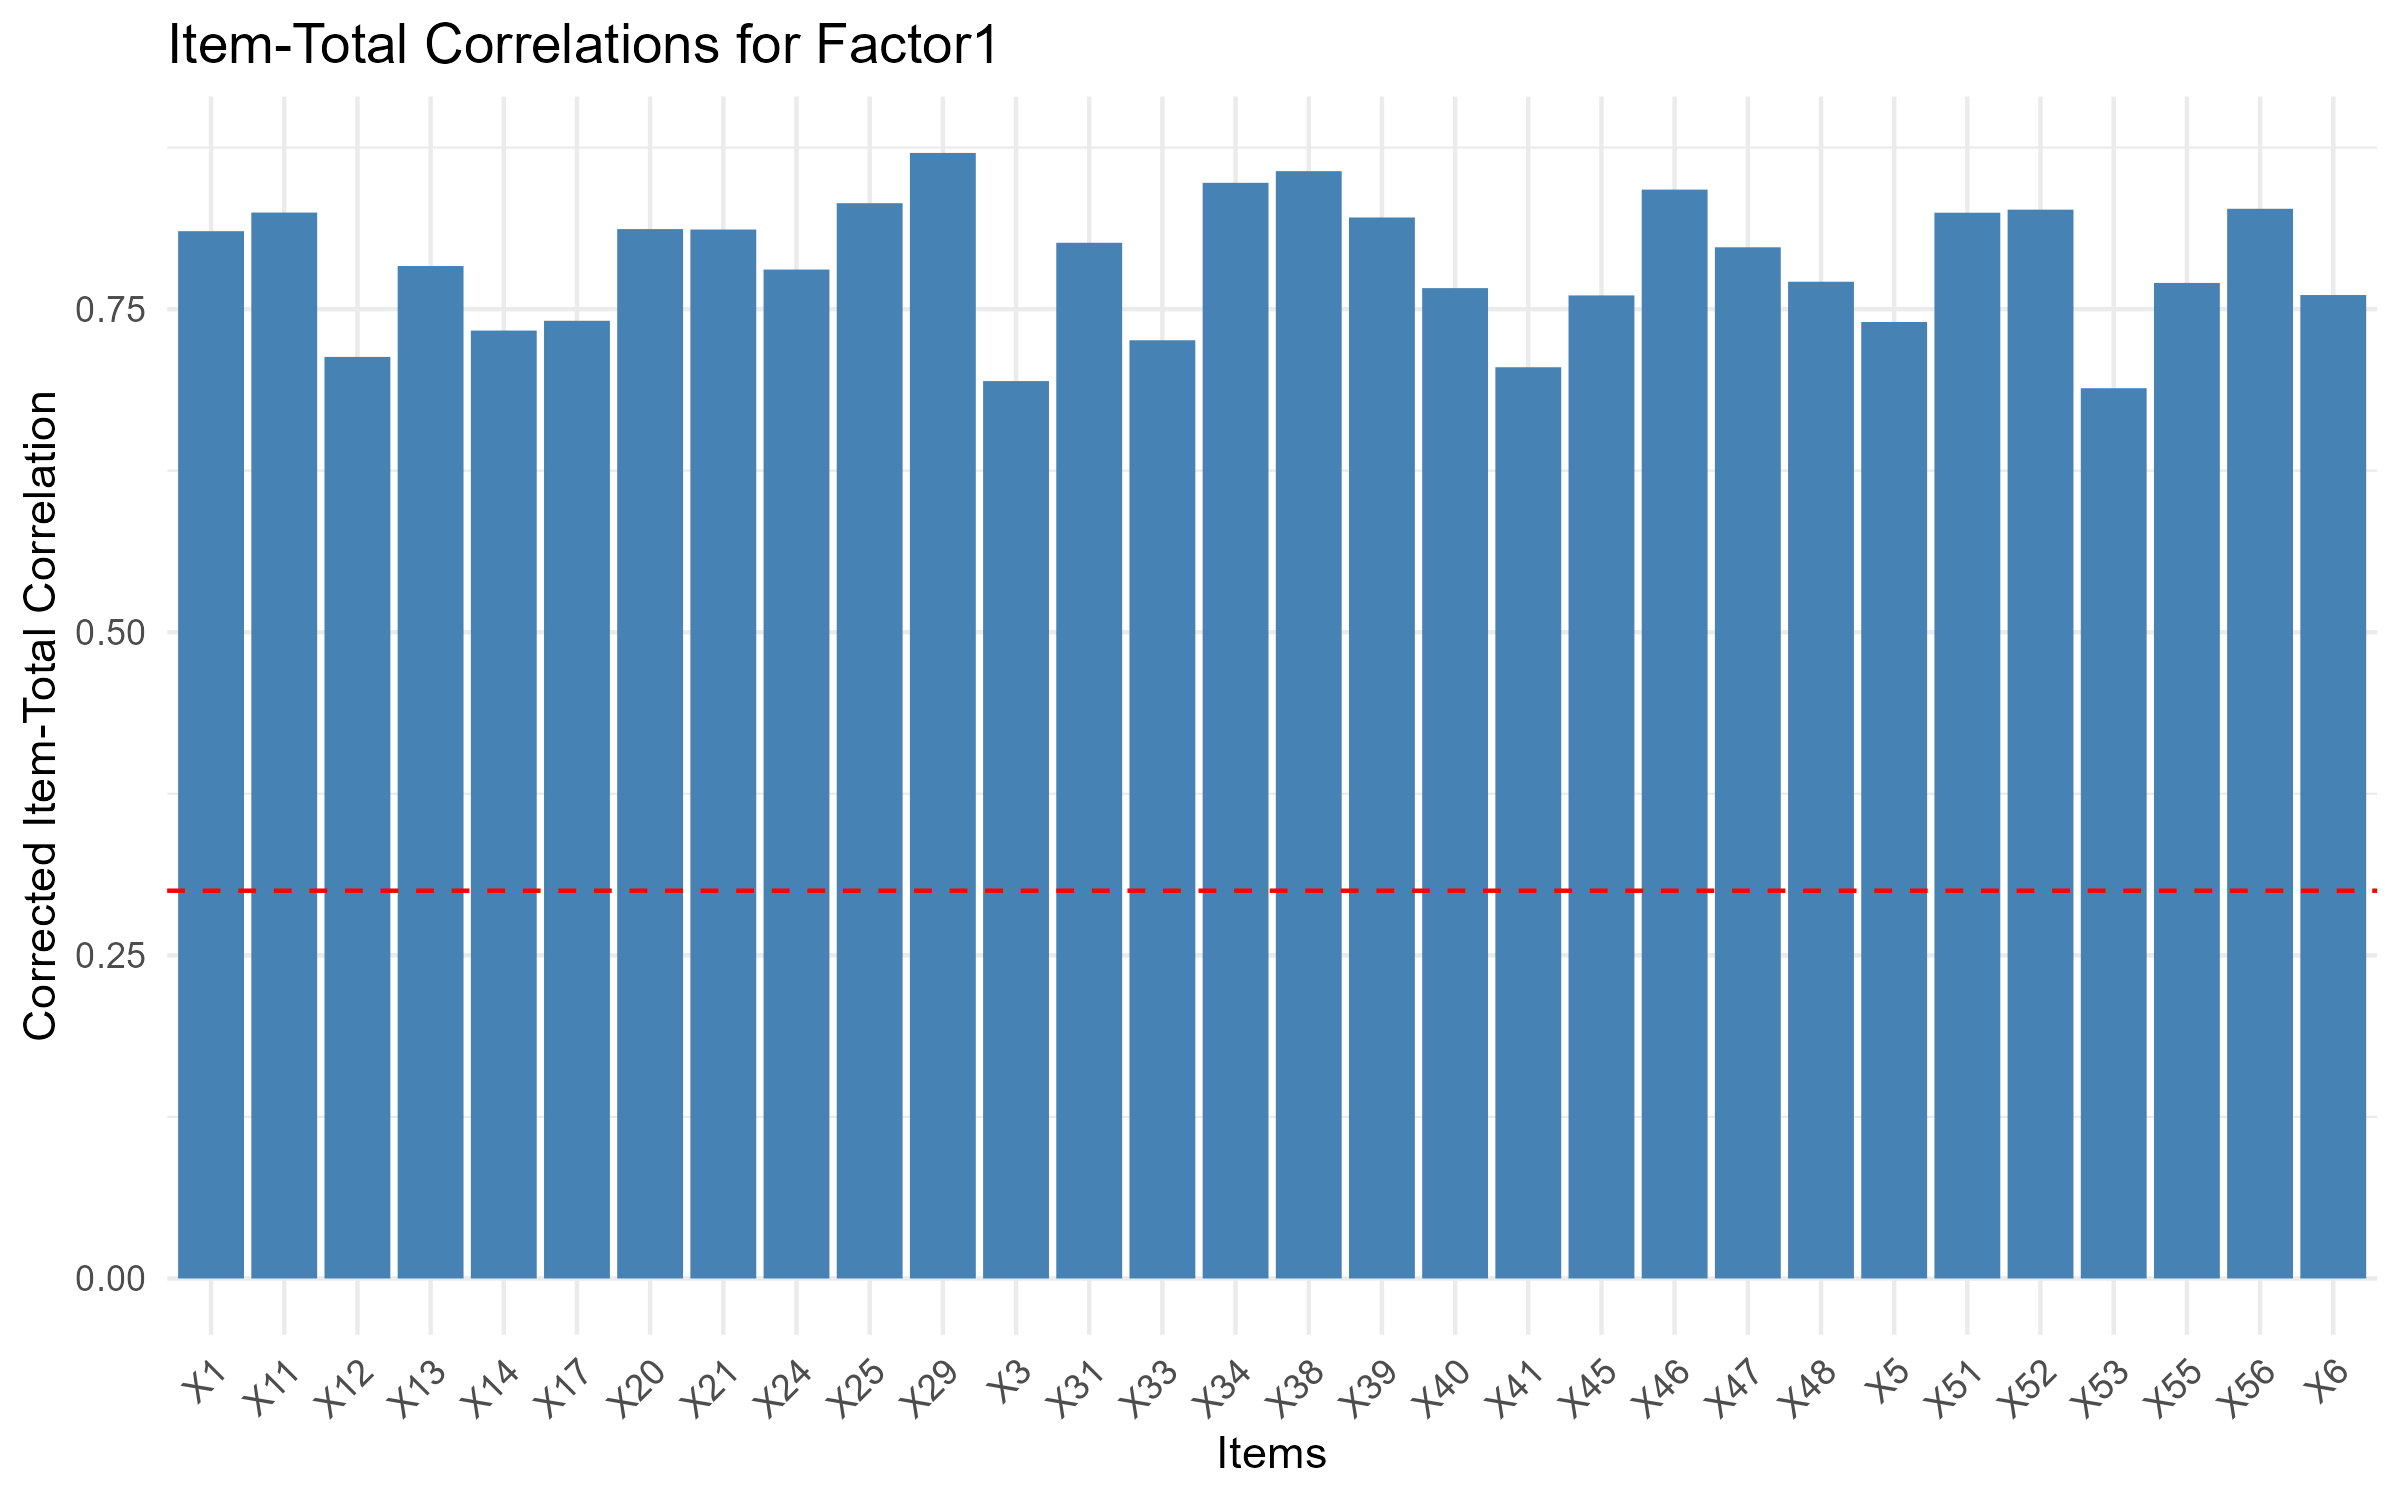
\includegraphics[width=\textwidth]{../../assets/images/reliability_Factor1.png}
        \caption{Độ tin cậy nhân tố 1}
    \end{minipage}
    \hfill
    \begin{minipage}{0.45\textwidth}
        \centering
        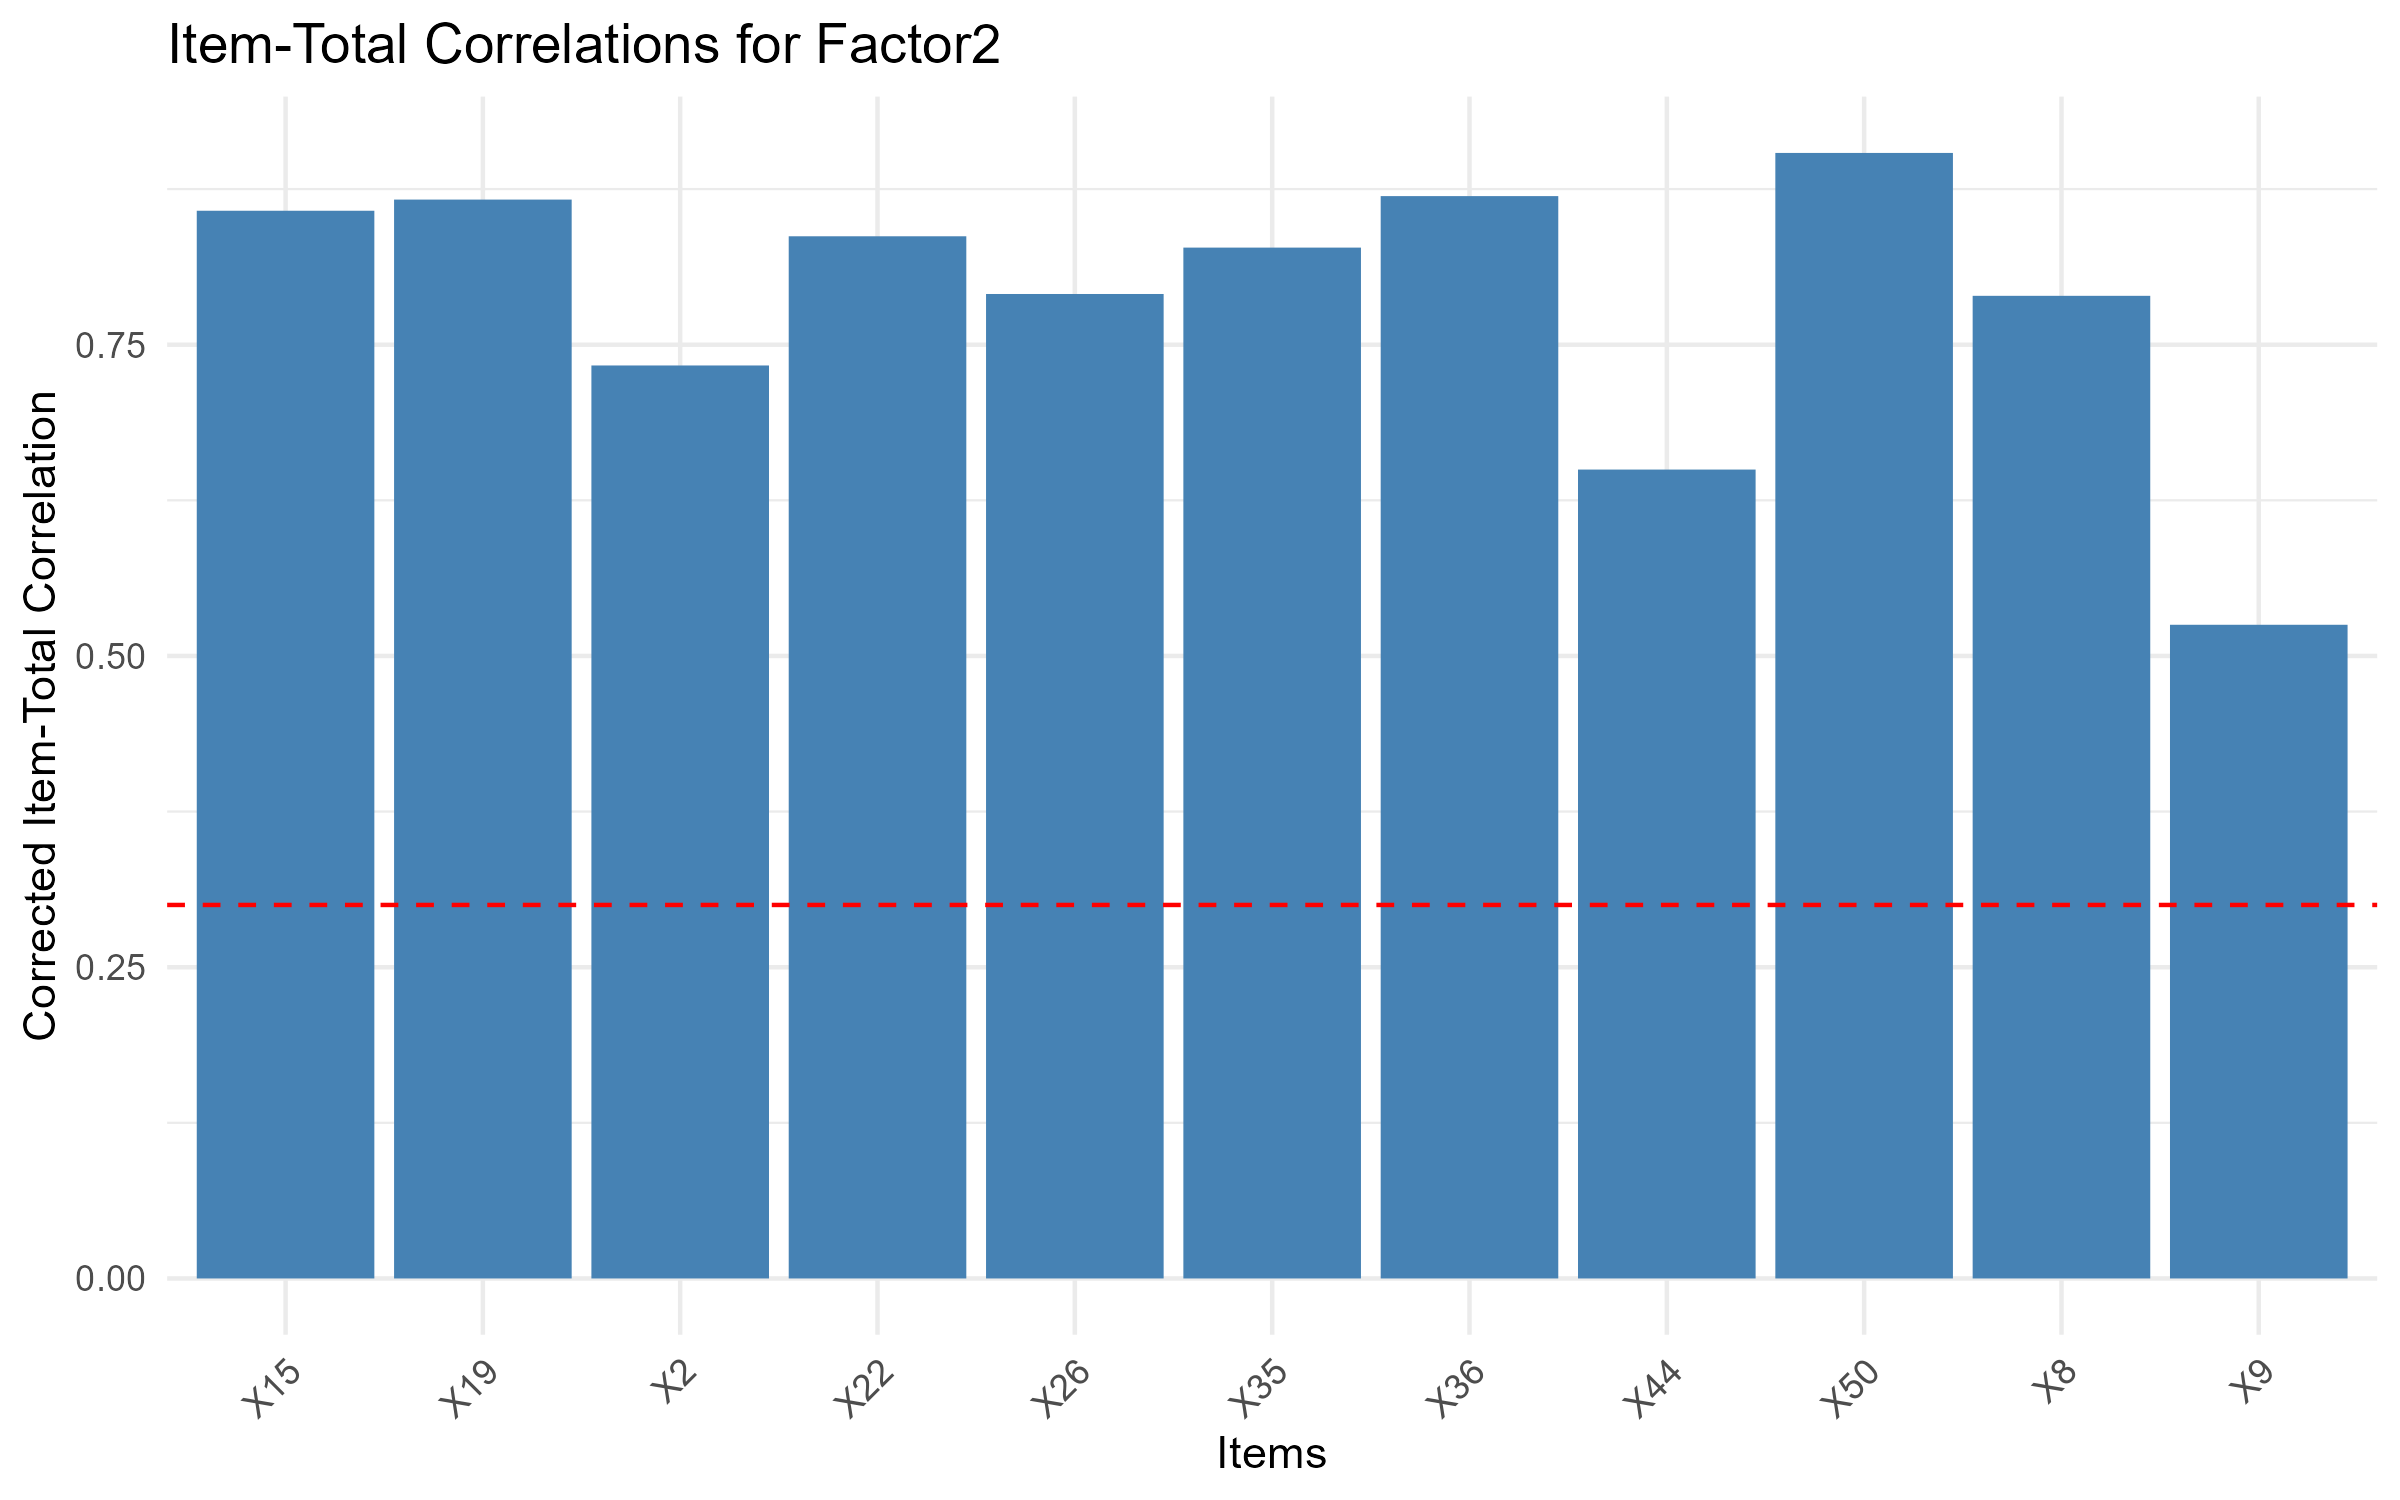
\includegraphics[width=\textwidth]{../../assets/images/reliability_Factor2.png}
        \caption{Độ tin cậy nhân tố 2}
    \end{minipage}
\end{figure}

\begin{figure}[h!]
    \centering
    \begin{minipage}{0.3\textwidth}
        \centering
        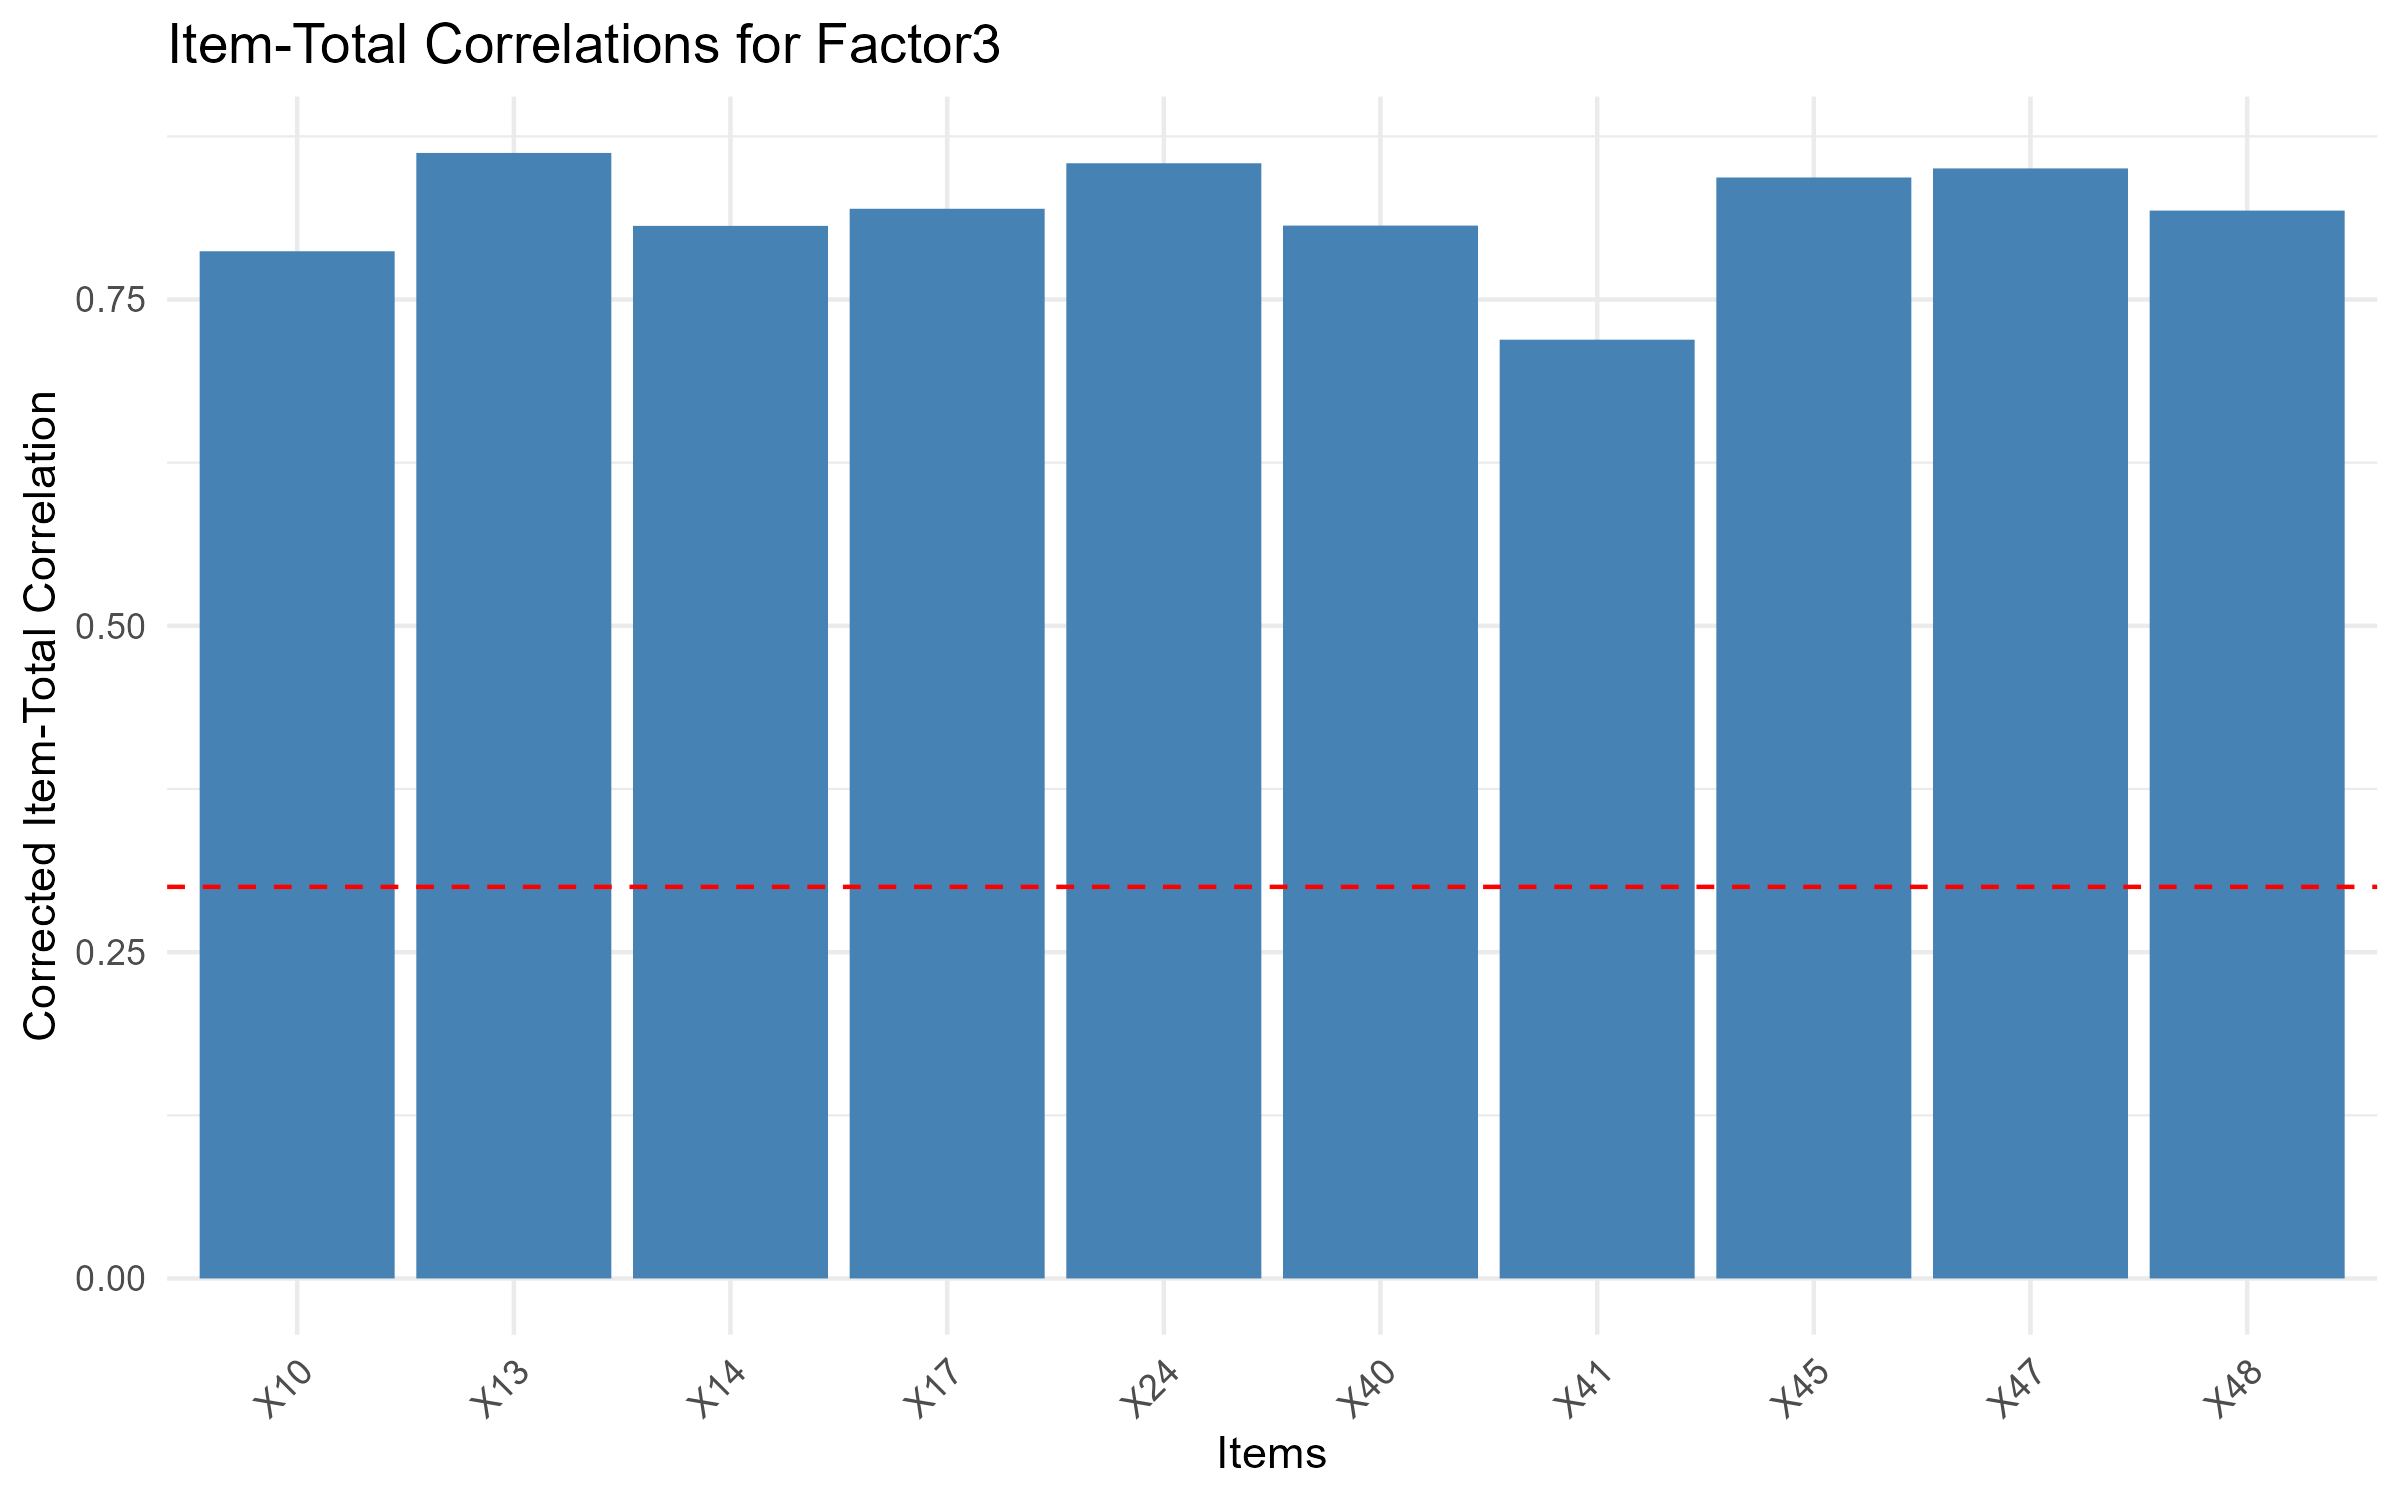
\includegraphics[width=\textwidth]{../../assets/images/reliability_Factor3.png}
        \caption{Độ tin cậy nhân tố 3}
    \end{minipage}
    \hfill
    \begin{minipage}{0.3\textwidth}
        \centering
        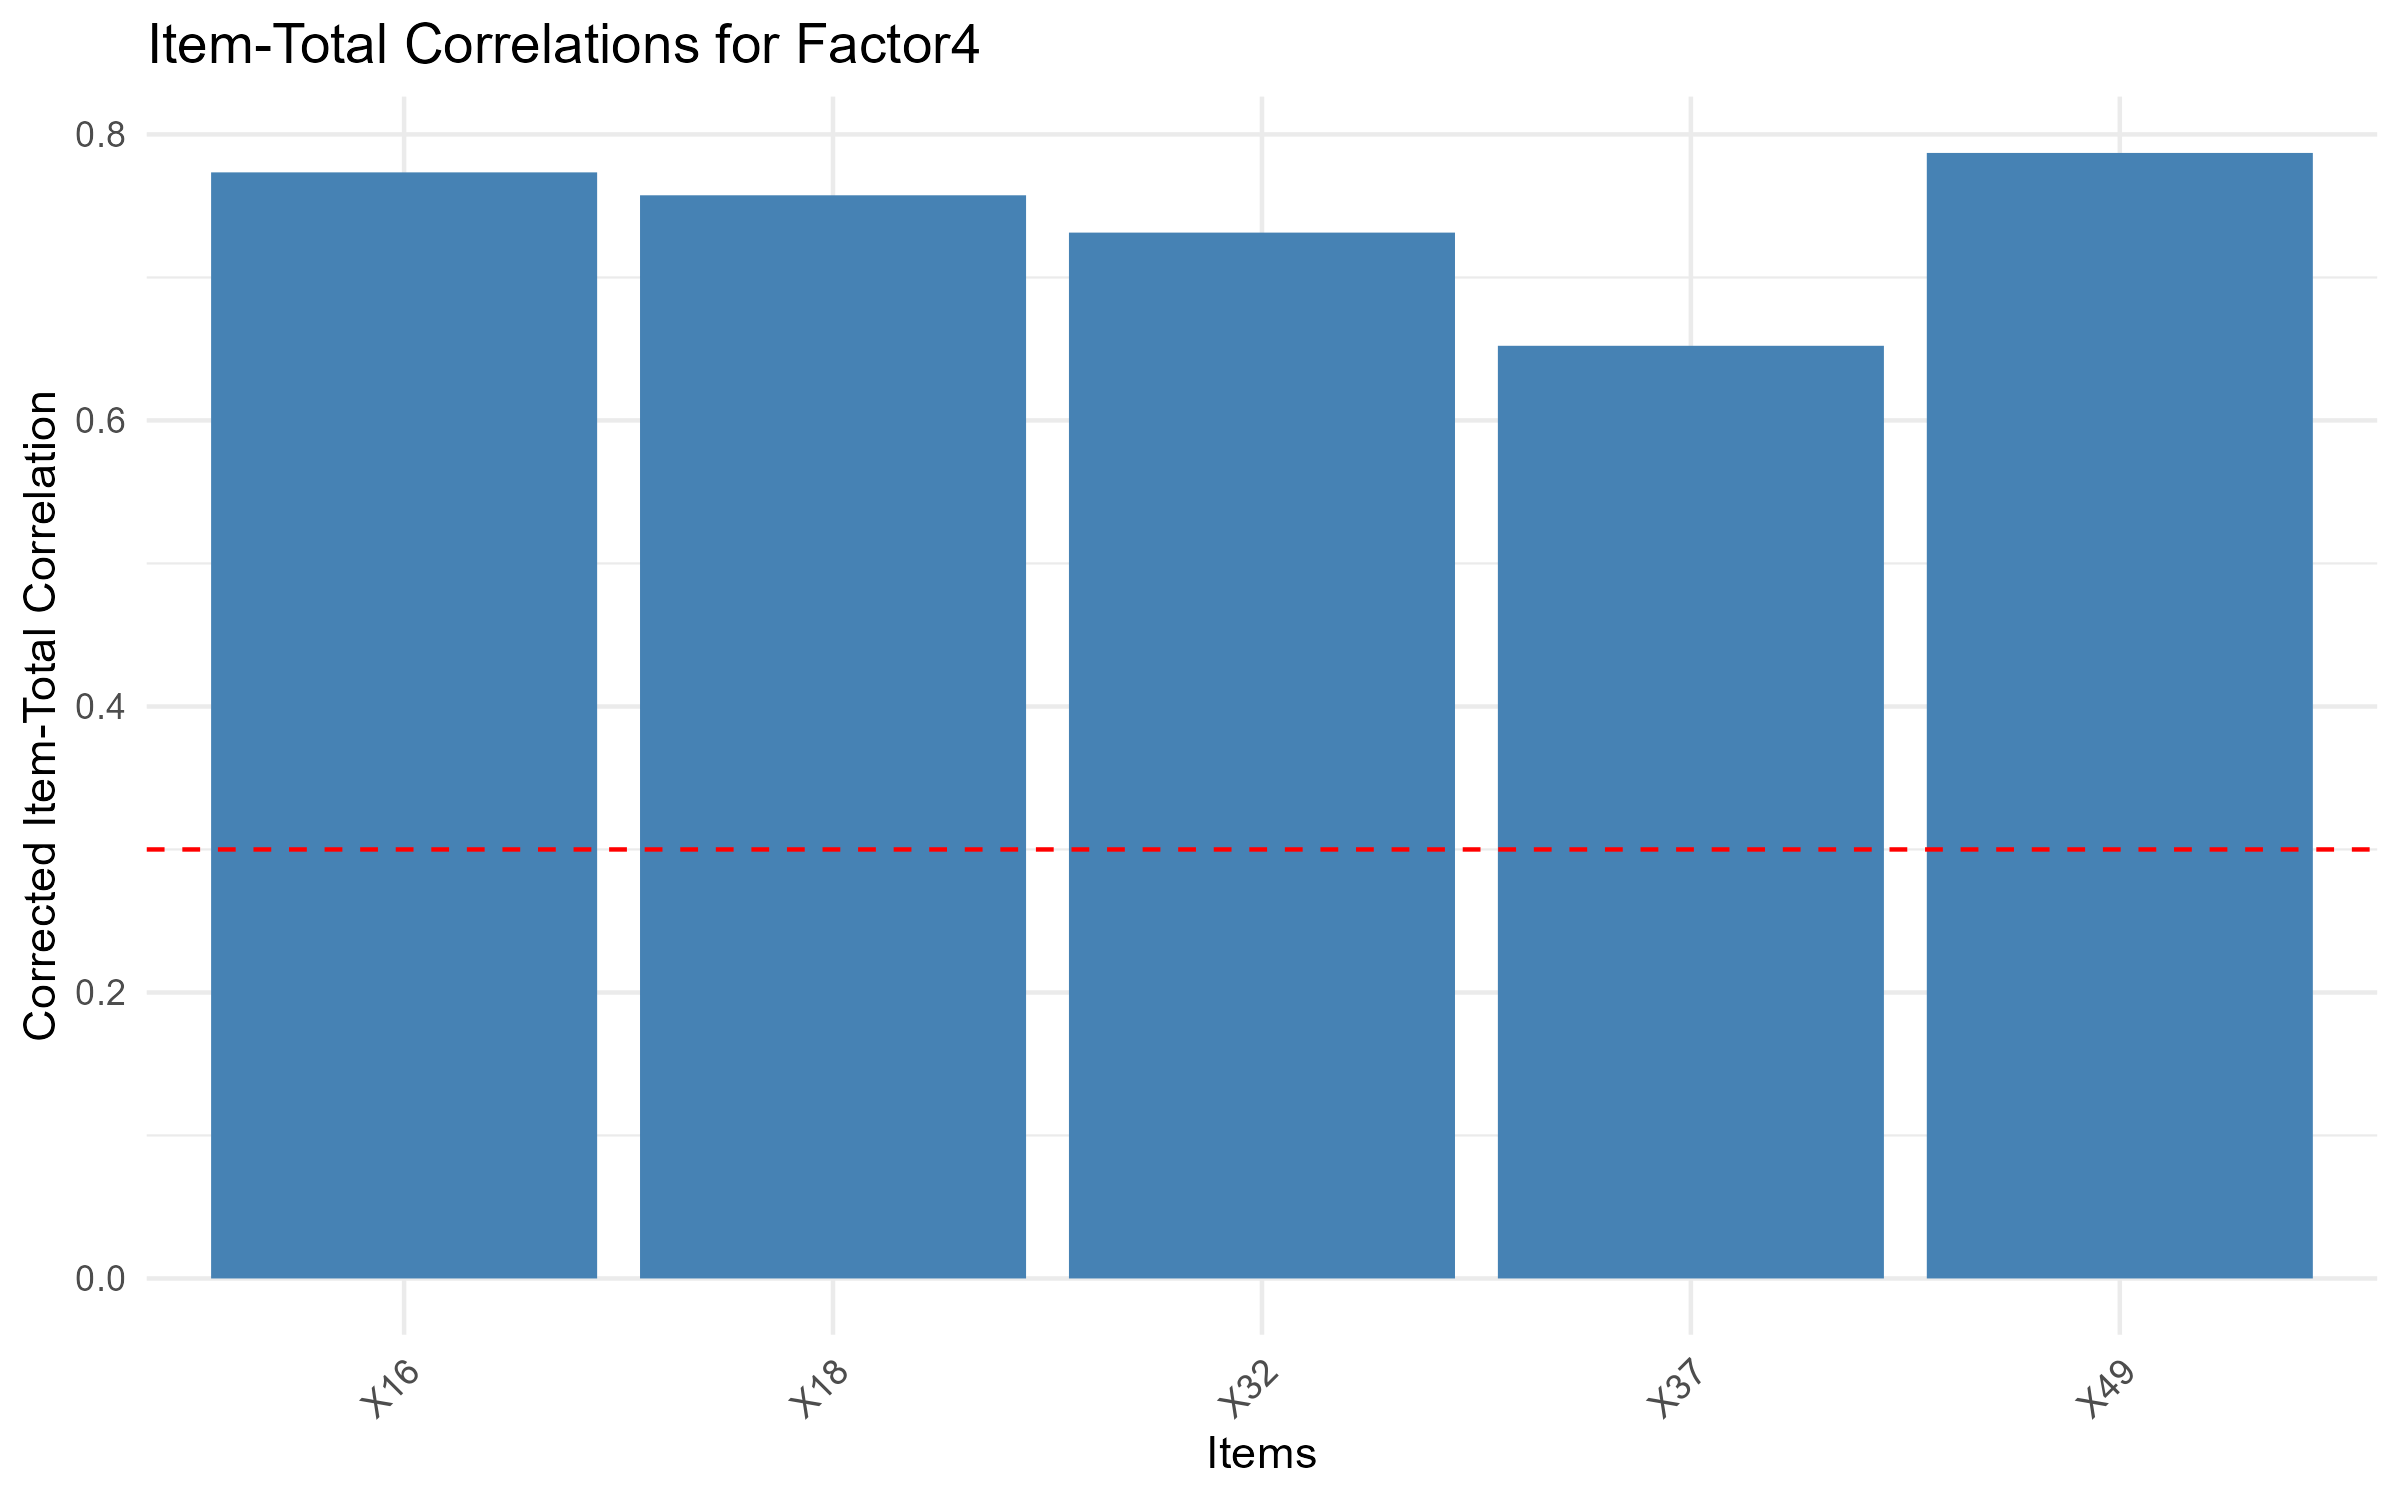
\includegraphics[width=\textwidth]{../../assets/images/reliability_Factor4.png}
        \caption{Độ tin cậy nhân tố 4}
    \end{minipage}
    \hfill
    \begin{minipage}{0.3\textwidth}
        \centering
        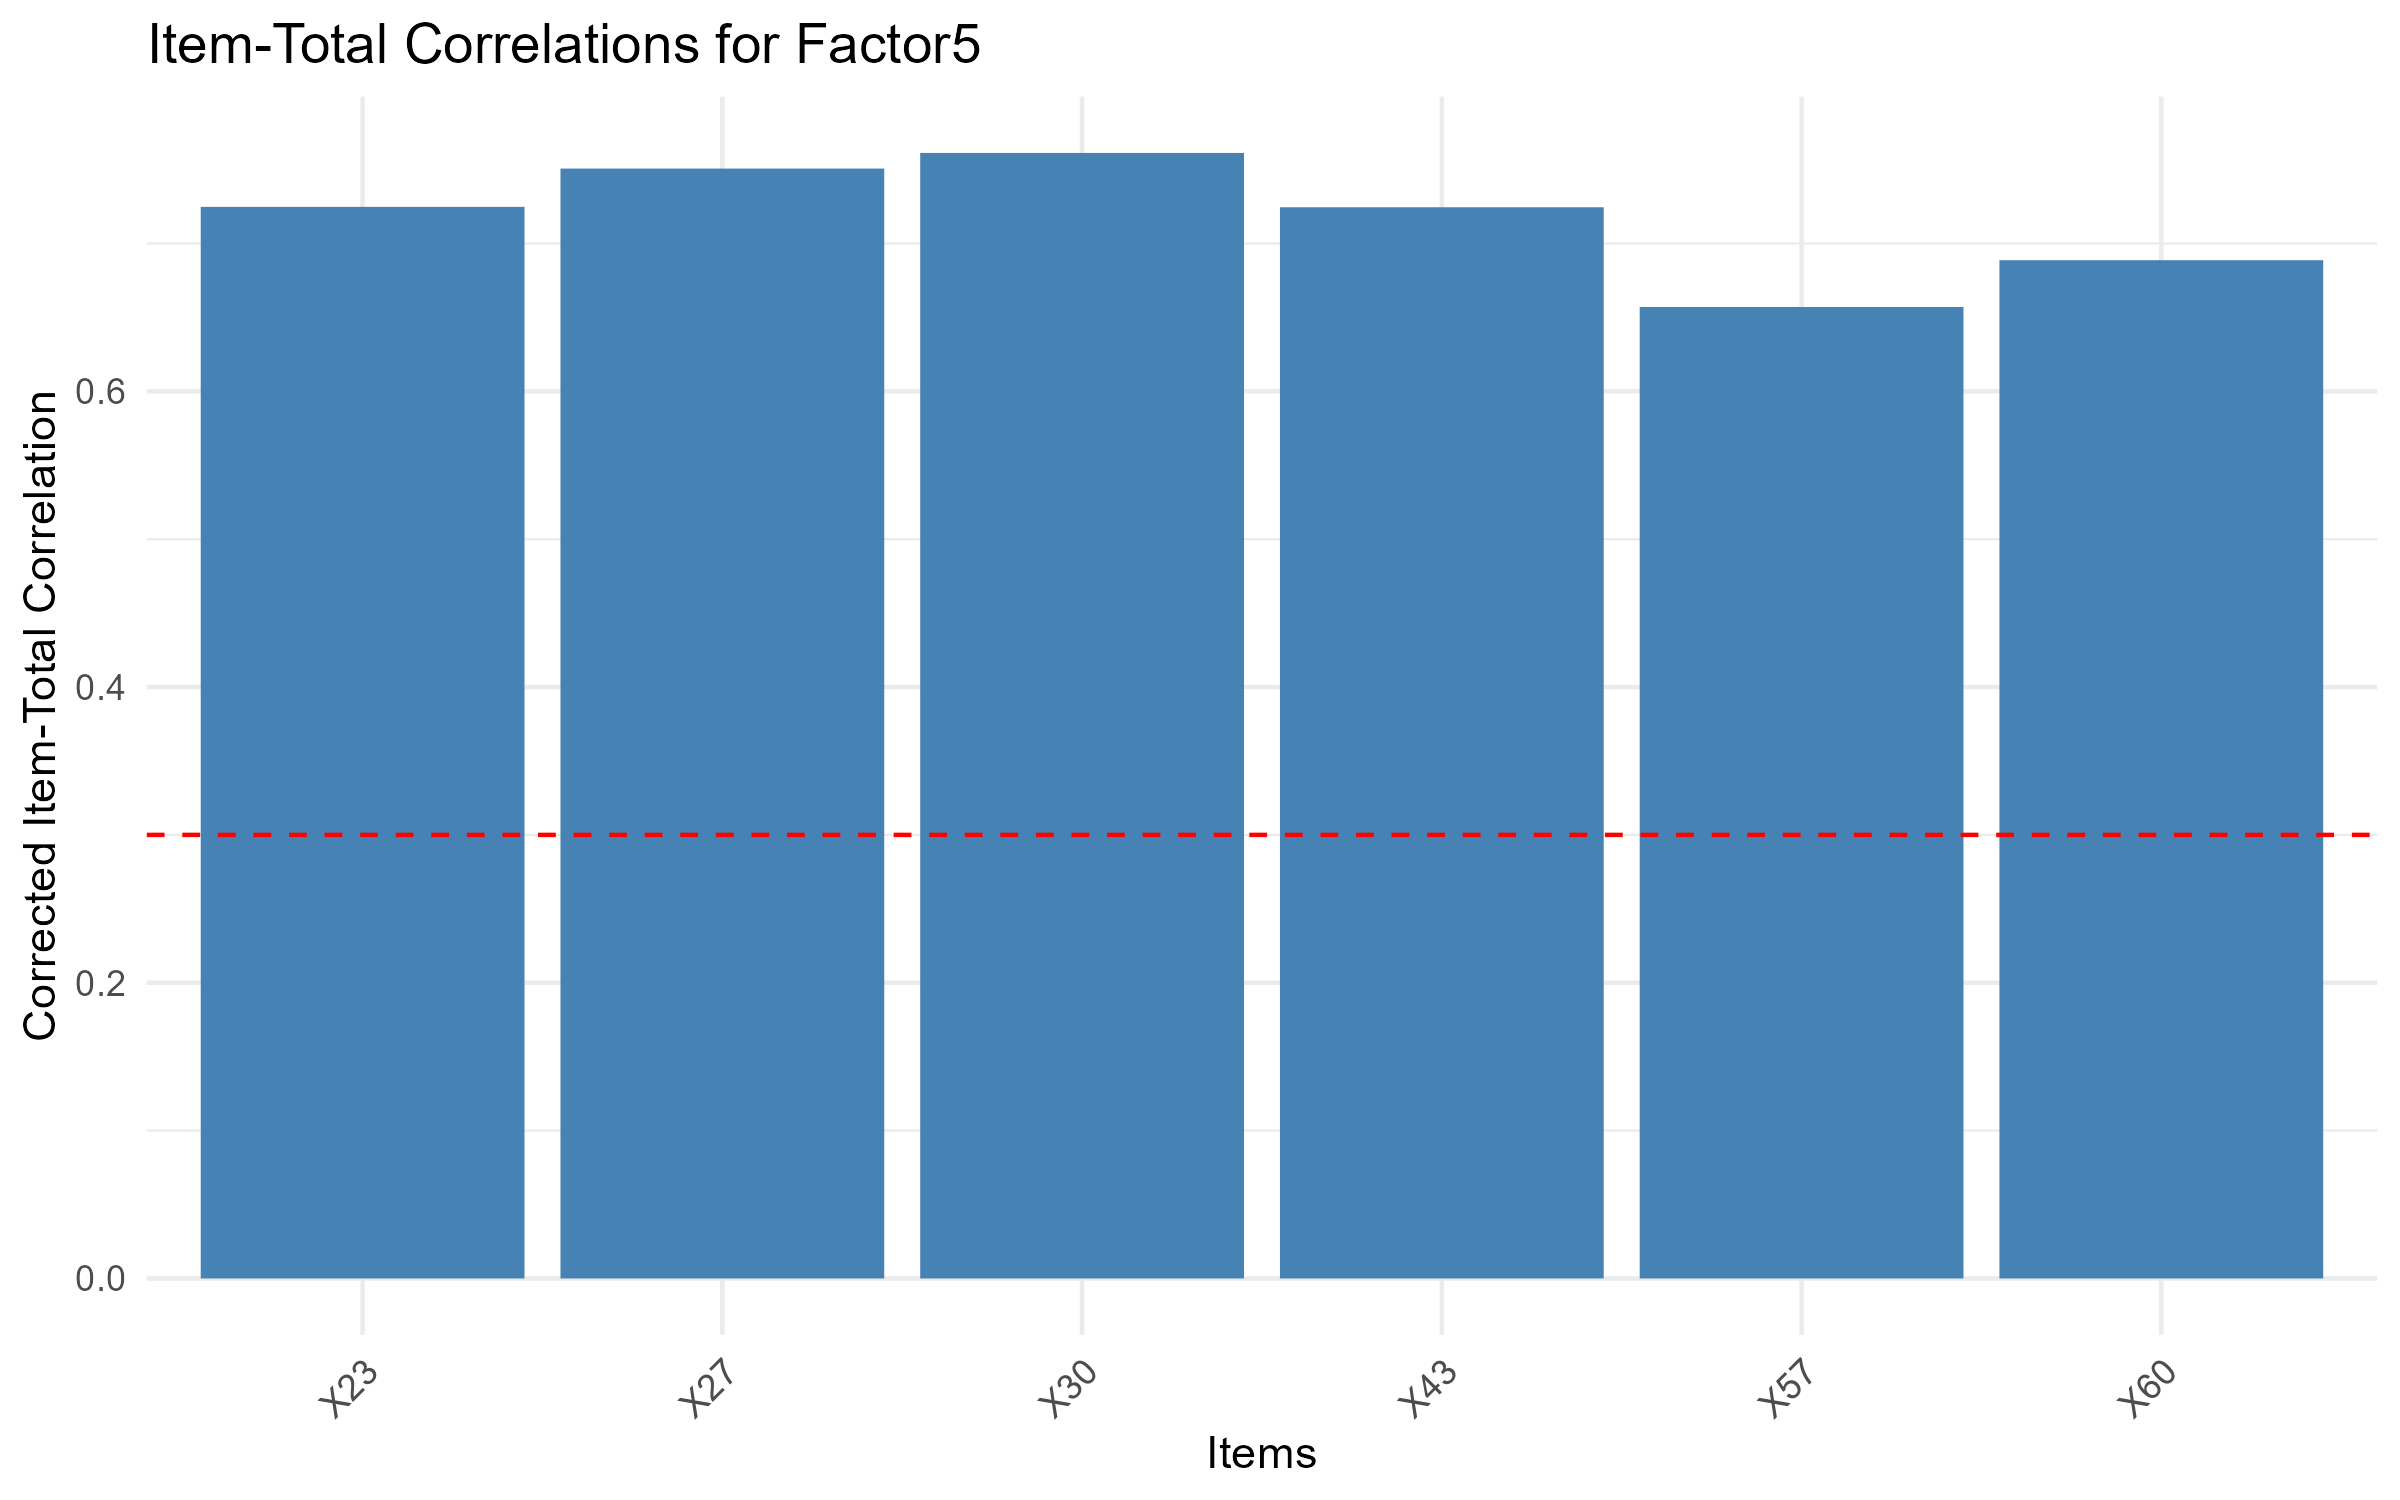
\includegraphics[width=\textwidth]{../../assets/images/reliability_Factor5.png}
        \caption{Độ tin cậy nhân tố 5}
    \end{minipage}
\end{figure}



\section{Kết luận chương}

Chương này đã trình bày một cách hệ thống các phương pháp phân tích dữ liệu nhiều chiều quan trọng. Những điểm chính cần ghi nhớ:

\begin{itemize}
    \item \textbf{PCA} phù hợp cho giảm chiều và trực quan hóa dữ liệu
    \item \textbf{Factor Analysis} tập trung vào tìm cấu trúc tiềm ẩn trong dữ liệu quan sát
    \item \textbf{EFA} giúp khám phá số lượng và bản chất của các nhân tố ẩn
    \item Đánh giá độ tin cậy bằng Cronbach's Alpha để đảm bảo tính nhất quán nội bộ
    \item Việc kết hợp nhiều phương pháp thường cho hiểu biết sâu sắc hơn về dữ liệu
    \item Cần validation kỹ lưỡng để đảm bảo tính tin cậy của kết quả
\end{itemize}

Các kỹ thuật này tạo thành nền tảng vững chắc cho việc phân tích dữ liệu phức tạp, từ nghiên cứu khoa học đến các ứng dụng thực tiễn trong nhiều lĩnh vực khác nhau.